\batchmode
\documentclass[letterpaper]{book}
\usepackage{makeidx}
\usepackage{fancyhdr}
\usepackage{graphicx}
\usepackage{multicol}
\usepackage{float}
\usepackage{textcomp}
\usepackage{alltt}
\ifx\pdfoutput\undefined
\usepackage[ps2pdf,
            pagebackref=true,
            colorlinks=true,
            linkcolor=blue
           ]{hyperref}
\usepackage{pspicture}
\else
\usepackage[pdftex,
            pagebackref=true,
            colorlinks=true,
            linkcolor=blue
           ]{hyperref}
\fi
\usepackage{doxygen}
\makeindex
\setcounter{tocdepth}{1}
\renewcommand{\footrulewidth}{0.4pt}
\begin{document}
\begin{titlepage}
\vspace*{7cm}
\begin{center}
{\Large @PACKAGE\_\-NAME@ Reference Manual\\[1ex]\large Version \begin{Desc}
\item[Version:]@ \end{Desc}
}\\
\vspace*{1cm}
{\large Generated by Doxygen 1.4.4}\\
\vspace*{0.5cm}
{\small Thu Jul 13 16:41:46 2006}\\
\end{center}
\end{titlepage}
\clearemptydoublepage
\pagenumbering{roman}
\tableofcontents
\clearemptydoublepage
\pagenumbering{arabic}
\chapter{Database Primitives Library }
\label{index}\hypertarget{index}{}\input{index}
\chapter{@PACKAGE\_\-NAME@ Module Index}
\input{modules}
\chapter{@PACKAGE\_\-NAME@ Directory Hierarchy}
\section{@PACKAGE\_\-NAME@ Directories}
This directory hierarchy is sorted roughly, but not completely, alphabetically:\begin{CompactList}
\item \contentsline{section}{tests}{\pageref{dir_000000}}{}
\end{CompactList}

\chapter{@PACKAGE\_\-NAME@ Data Structure Index}
\input{annotated}
\chapter{@PACKAGE\_\-NAME@ File Index}
\input{files}
\chapter{@PACKAGE\_\-NAME@ Module Documentation}
\hypertarget{group__dbprim}{
\section{Database Primitives}
\label{group__dbprim}\index{Database Primitives@{Database Primitives}}
}


\subsection{Detailed Description}
This module describes interfaces common to all database modules--mainly the macros concerned with manipulating database keys and the definition of the key structure.

The key may be any arbitrary pointer, including a pointer to a string. Everything that handles a key either copies the contents of the \hyperlink{group__dbprim_a0}{db\_\-key\_\-t} structure or passes it to a user-defined function. If required, as in the case of a string, a length may also be represented in the key structure. \subsection*{Defines}
\begin{CompactItemize}
\item 
\#define \hyperlink{group__dbprim_a1}{DB\_\-KEY\_\-INIT}(key, size)
\begin{CompactList}\small\item\em Database key static initializer.\item\end{CompactList}\item 
\#define \hyperlink{group__dbprim_a2}{dk\_\-key}(key)
\begin{CompactList}\small\item\em Database key accessor macro.\item\end{CompactList}\item 
\#define \hyperlink{group__dbprim_a3}{dk\_\-len}(key)
\begin{CompactList}\small\item\em Database key length accessor macro.\item\end{CompactList}\item 
\#define \hyperlink{group__dbprim_a4}{DB\_\-FLAG\_\-REVERSE}
\begin{CompactList}\small\item\em Reverse flag.\item\end{CompactList}\end{CompactItemize}
\subsection*{Typedefs}
\begin{CompactItemize}
\item 
typedef \_\-db\_\-key\_\-s \hyperlink{group__dbprim_a0}{db\_\-key\_\-t}
\begin{CompactList}\small\item\em Database key.\item\end{CompactList}\end{CompactItemize}


\subsection{Define Documentation}
\hypertarget{group__dbprim_a4}{
\index{dbprim@{dbprim}!DB_FLAG_REVERSE@{DB\_\-FLAG\_\-REVERSE}}
\index{DB_FLAG_REVERSE@{DB\_\-FLAG\_\-REVERSE}!dbprim@{dbprim}}
\subsubsection[DB\_\-FLAG\_\-REVERSE]{\setlength{\rightskip}{0pt plus 5cm}\#define DB\_\-FLAG\_\-REVERSE}}
\label{group__dbprim_a4}


This flag can be passed to ordered iterations to reverse the order of the iterations. \hypertarget{group__dbprim_a1}{
\index{dbprim@{dbprim}!DB_KEY_INIT@{DB\_\-KEY\_\-INIT}}
\index{DB_KEY_INIT@{DB\_\-KEY\_\-INIT}!dbprim@{dbprim}}
\subsubsection[DB\_\-KEY\_\-INIT]{\setlength{\rightskip}{0pt plus 5cm}\#define DB\_\-KEY\_\-INIT(key, size)}}
\label{group__dbprim_a1}


This macro allows a \hyperlink{group__dbprim_a0}{db\_\-key\_\-t} to be initialized statically.\begin{Desc}
\item[Parameters: ]\par
\begin{description}
\item[{\em 
key}]A pointer to the key. \item[{\em 
size}]Size of the key. \end{description}
\end{Desc}
\hypertarget{group__dbprim_a2}{
\index{dbprim@{dbprim}!dk_key@{dk\_\-key}}
\index{dk_key@{dk\_\-key}!dbprim@{dbprim}}
\subsubsection[dk\_\-key]{\setlength{\rightskip}{0pt plus 5cm}\#define dk\_\-key(key)}}
\label{group__dbprim_a2}


This macro allows access to the key field of a \hyperlink{group__dbprim_a0}{db\_\-key\_\-t}. It may be used as an lvalue in order to assign a key to a \hyperlink{group__dbprim_a0}{db\_\-key\_\-t}.\begin{Desc}
\item[Parameters: ]\par
\begin{description}
\item[{\em 
key}]A pointer to a \hyperlink{group__dbprim_a0}{db\_\-key\_\-t}. \end{description}
\end{Desc}
\begin{Desc}
\item[Returns: ]\par
A pointer to a key ({\tt void $\ast$}). \end{Desc}
\hypertarget{group__dbprim_a3}{
\index{dbprim@{dbprim}!dk_len@{dk\_\-len}}
\index{dk_len@{dk\_\-len}!dbprim@{dbprim}}
\subsubsection[dk\_\-len]{\setlength{\rightskip}{0pt plus 5cm}\#define dk\_\-len(key)}}
\label{group__dbprim_a3}


This macro allows access to the key length field of a \hyperlink{group__dbprim_a0}{db\_\-key\_\-t}. It may be used as an lvalue in order to assign a length to a \hyperlink{group__dbprim_a0}{db\_\-key\_\-t}.\begin{Desc}
\item[Parameters: ]\par
\begin{description}
\item[{\em 
key}]A pointer to a \hyperlink{group__dbprim_a0}{db\_\-key\_\-t}. \end{description}
\end{Desc}
\begin{Desc}
\item[Returns: ]\par
An {\tt int} describing the length of the key. \end{Desc}


\subsection{Typedef Documentation}
\hypertarget{group__dbprim_a0}{
\index{dbprim@{dbprim}!db_key_t@{db\_\-key\_\-t}}
\index{db_key_t@{db\_\-key\_\-t}!dbprim@{dbprim}}
\subsubsection[db\_\-key\_\-t]{\setlength{\rightskip}{0pt plus 5cm}typedef struct \_\-db\_\-key\_\-s db\_\-key\_\-t}}
\label{group__dbprim_a0}


This structure is a generic key containing a void $\ast$ pointer and a length parameter. It should be accessed with $\ast$ \hyperlink{group__dbprim_a2}{dk\_\-key()} and \hyperlink{group__dbprim_a3}{dk\_\-len()}. 
\hypertarget{group__dbprim__link}{
\section{Linked lists}
\label{group__dbprim__link}\index{Linked lists@{Linked lists}}
}


\subsection{Detailed Description}
Linked lists are a very basic data structure used in building databases. This library provides a simple yet powerful implementation of generic linked lists, based on two caller-allocated structures. The \hyperlink{group__dbprim__link_a0}{link\_\-head\_\-t} structure describes the head of a linked list and contains information regarding the number of elements in the linked list as well as pointers referencing the first and last elements in the list. The \hyperlink{group__dbprim__link_a1}{link\_\-elem\_\-t} structure describes a specific element in the linked list and contains pointers referencing the next and previous elements in the list, as well as a pointer to the object, a pointer to the head of the linked list, and a set of user-specified flags.

Elements may be added at any arbitrary location in the linked list with \hyperlink{group__dbprim__link_a6}{ll\_\-add()}; moved to any other arbitrary location in the linked list with \hyperlink{group__dbprim__link_a7}{ll\_\-move()}; or removed from the list with \hyperlink{group__dbprim__link_a8}{ll\_\-remove()}. In addition, the user may search the list using a user-defined comparison function with \hyperlink{group__dbprim__link_a9}{ll\_\-find()}; iterate over every element in the list with \hyperlink{group__dbprim__link_a10}{ll\_\-iter()}; or remove all items from the list with \hyperlink{group__dbprim__link_a11}{ll\_\-flush()}, optionally executing a user-specified clean-up function. \subsection*{Defines}
\begin{CompactItemize}
\item 
\#define \hyperlink{group__dbprim__link_a13}{LINK\_\-HEAD\_\-INIT}(extra)
\begin{CompactList}\small\item\em Linked list head static initializer.\item\end{CompactList}\item 
\#define \hyperlink{group__dbprim__link_a14}{ll\_\-verify}(list)
\begin{CompactList}\small\item\em Linked list head verification macro.\item\end{CompactList}\item 
\#define \hyperlink{group__dbprim__link_a15}{ll\_\-count}(list)
\begin{CompactList}\small\item\em Linked list count.\item\end{CompactList}\item 
\#define \hyperlink{group__dbprim__link_a16}{ll\_\-first}(list)
\begin{CompactList}\small\item\em First element in linked list.\item\end{CompactList}\item 
\#define \hyperlink{group__dbprim__link_a17}{ll\_\-last}(list)
\begin{CompactList}\small\item\em Last element in a linked list.\item\end{CompactList}\item 
\#define \hyperlink{group__dbprim__link_a18}{ll\_\-extra}(list)
\begin{CompactList}\small\item\em Extra pointer data in a linked list.\item\end{CompactList}\item 
\#define \hyperlink{group__dbprim__link_a19}{LINK\_\-ELEM\_\-INIT}(obj)
\begin{CompactList}\small\item\em Linked list element static initializer.\item\end{CompactList}\item 
\#define \hyperlink{group__dbprim__link_a20}{le\_\-verify}(element)
\begin{CompactList}\small\item\em Linked list element verification macro.\item\end{CompactList}\item 
\#define \hyperlink{group__dbprim__link_a21}{le\_\-next}(elem)
\begin{CompactList}\small\item\em Linked list element next pointer.\item\end{CompactList}\item 
\#define \hyperlink{group__dbprim__link_a22}{le\_\-prev}(elem)
\begin{CompactList}\small\item\em Linked list element previous pointer.\item\end{CompactList}\item 
\#define \hyperlink{group__dbprim__link_a23}{le\_\-object}(elem)
\begin{CompactList}\small\item\em Linked list element object pointer.\item\end{CompactList}\item 
\#define \hyperlink{group__dbprim__link_a24}{le\_\-head}(elem)
\begin{CompactList}\small\item\em Linked list element head pointer.\item\end{CompactList}\item 
\#define \hyperlink{group__dbprim__link_a25}{le\_\-flags}(elem)
\begin{CompactList}\small\item\em Linked list element flags.\item\end{CompactList}\end{CompactItemize}
\subsection*{Typedefs}
\begin{CompactItemize}
\item 
typedef \_\-link\_\-head\_\-s \hyperlink{group__dbprim__link_a0}{link\_\-head\_\-t}
\begin{CompactList}\small\item\em Linked list head.\item\end{CompactList}\item 
typedef \_\-link\_\-elem\_\-s \hyperlink{group__dbprim__link_a1}{link\_\-elem\_\-t}
\begin{CompactList}\small\item\em Linked list element.\item\end{CompactList}\item 
typedef unsigned long($\ast$ \hyperlink{group__dbprim__link_a2}{link\_\-iter\_\-t} )(\hyperlink{group__dbprim__link_a0}{link\_\-head\_\-t} $\ast$, \hyperlink{group__dbprim__link_a1}{link\_\-elem\_\-t} $\ast$, void $\ast$)
\begin{CompactList}\small\item\em Linked list iteration callback.\item\end{CompactList}\item 
typedef unsigned long($\ast$ \hyperlink{group__dbprim__link_a3}{link\_\-comp\_\-t} )(\hyperlink{group__dbprim_a0}{db\_\-key\_\-t} $\ast$, void $\ast$)
\begin{CompactList}\small\item\em Linked list comparison callback.\item\end{CompactList}\item 
typedef enum \hyperlink{group__dbprim__link_a26}{\_\-link\_\-loc\_\-e} \hyperlink{group__dbprim__link_a4}{link\_\-loc\_\-t}
\begin{CompactList}\small\item\em Linked list location.\item\end{CompactList}\end{CompactItemize}
\subsection*{Enumerations}
\begin{CompactItemize}
\item 
enum \hyperlink{group__dbprim__link_a26}{\_\-link\_\-loc\_\-e} \{ \hyperlink{group__dbprim__link_a26a132}{LINK\_\-LOC\_\-HEAD}, 
\hyperlink{group__dbprim__link_a26a133}{LINK\_\-LOC\_\-TAIL}, 
\hyperlink{group__dbprim__link_a26a134}{LINK\_\-LOC\_\-BEFORE}, 
\hyperlink{group__dbprim__link_a26a135}{LINK\_\-LOC\_\-AFTER}
 \}
\begin{CompactList}\small\item\em Linked list location.\item\end{CompactList}\end{CompactItemize}
\subsection*{Functions}
\begin{CompactItemize}
\item 
unsigned long \hyperlink{group__dbprim__link_a5}{ll\_\-init} (\hyperlink{group__dbprim__link_a0}{link\_\-head\_\-t} $\ast$list, void $\ast$extra)
\begin{CompactList}\small\item\em Dynamically initialize a linked list head.\item\end{CompactList}\item 
unsigned long \hyperlink{group__dbprim__link_a6}{ll\_\-add} (\hyperlink{group__dbprim__link_a0}{link\_\-head\_\-t} $\ast$list, \hyperlink{group__dbprim__link_a1}{link\_\-elem\_\-t} $\ast$new, \hyperlink{group__dbprim__link_a4}{link\_\-loc\_\-t} loc, \hyperlink{group__dbprim__link_a1}{link\_\-elem\_\-t} $\ast$elem)
\begin{CompactList}\small\item\em Add an element to a linked list.\item\end{CompactList}\item 
unsigned long \hyperlink{group__dbprim__link_a7}{ll\_\-move} (\hyperlink{group__dbprim__link_a0}{link\_\-head\_\-t} $\ast$list, \hyperlink{group__dbprim__link_a1}{link\_\-elem\_\-t} $\ast$new, \hyperlink{group__dbprim__link_a4}{link\_\-loc\_\-t} loc, \hyperlink{group__dbprim__link_a1}{link\_\-elem\_\-t} $\ast$elem)
\begin{CompactList}\small\item\em Move an element within a linked list.\item\end{CompactList}\item 
unsigned long \hyperlink{group__dbprim__link_a8}{ll\_\-remove} (\hyperlink{group__dbprim__link_a0}{link\_\-head\_\-t} $\ast$list, \hyperlink{group__dbprim__link_a1}{link\_\-elem\_\-t} $\ast$elem)
\begin{CompactList}\small\item\em Remove an element from a linked list.\item\end{CompactList}\item 
unsigned long \hyperlink{group__dbprim__link_a9}{ll\_\-find} (\hyperlink{group__dbprim__link_a0}{link\_\-head\_\-t} $\ast$list, \hyperlink{group__dbprim__link_a1}{link\_\-elem\_\-t} $\ast$$\ast$elem\_\-p, \hyperlink{group__dbprim__link_a3}{link\_\-comp\_\-t} comp\_\-func, \hyperlink{group__dbprim__link_a1}{link\_\-elem\_\-t} $\ast$start, \hyperlink{group__dbprim_a0}{db\_\-key\_\-t} $\ast$key)
\begin{CompactList}\small\item\em Find an element in a linked list.\item\end{CompactList}\item 
unsigned long \hyperlink{group__dbprim__link_a10}{ll\_\-iter} (\hyperlink{group__dbprim__link_a0}{link\_\-head\_\-t} $\ast$list, \hyperlink{group__dbprim__link_a1}{link\_\-elem\_\-t} $\ast$start, \hyperlink{group__dbprim__link_a2}{link\_\-iter\_\-t} iter\_\-func, void $\ast$extra, unsigned long flags)
\begin{CompactList}\small\item\em Iterate over each entry in a linked list.\item\end{CompactList}\item 
unsigned long \hyperlink{group__dbprim__link_a11}{ll\_\-flush} (\hyperlink{group__dbprim__link_a0}{link\_\-head\_\-t} $\ast$list, \hyperlink{group__dbprim__link_a2}{link\_\-iter\_\-t} flush\_\-func, void $\ast$extra)
\begin{CompactList}\small\item\em Flush a linked list.\item\end{CompactList}\item 
unsigned long \hyperlink{group__dbprim__link_a12}{le\_\-init} (\hyperlink{group__dbprim__link_a1}{link\_\-elem\_\-t} $\ast$elem, void $\ast$object)
\begin{CompactList}\small\item\em Dynamically initialize a linked list element.\item\end{CompactList}\end{CompactItemize}


\subsection{Define Documentation}
\hypertarget{group__dbprim__link_a25}{
\index{dbprim_link@{dbprim\_\-link}!le_flags@{le\_\-flags}}
\index{le_flags@{le\_\-flags}!dbprim_link@{dbprim\_\-link}}
\subsubsection[le\_\-flags]{\setlength{\rightskip}{0pt plus 5cm}\#define le\_\-flags(elem)}}
\label{group__dbprim__link_a25}


This macro retrieves a set of user-defined flags associated with the element. It may be used as an lvalue to set those flags.\begin{Desc}
\item[Parameters: ]\par
\begin{description}
\item[{\em 
elem}]A pointer to a \hyperlink{group__dbprim__link_a1}{link\_\-elem\_\-t}.\end{description}
\end{Desc}
\begin{Desc}
\item[Returns: ]\par
An {\tt unsigned long} containing the flags associated with the element. \end{Desc}
\hypertarget{group__dbprim__link_a24}{
\index{dbprim_link@{dbprim\_\-link}!le_head@{le\_\-head}}
\index{le_head@{le\_\-head}!dbprim_link@{dbprim\_\-link}}
\subsubsection[le\_\-head]{\setlength{\rightskip}{0pt plus 5cm}\#define le\_\-head(elem)}}
\label{group__dbprim__link_a24}


This macro retrieves a pointer to the head of the linked list that the element is in.\begin{Desc}
\item[Parameters: ]\par
\begin{description}
\item[{\em 
elem}]A pointer to a \hyperlink{group__dbprim__link_a1}{link\_\-elem\_\-t}.\end{description}
\end{Desc}
\begin{Desc}
\item[Returns: ]\par
A pointer to a \hyperlink{group__dbprim__link_a0}{link\_\-head\_\-t} representing the head of the linked list the element is in. \end{Desc}
\hypertarget{group__dbprim__link_a21}{
\index{dbprim_link@{dbprim\_\-link}!le_next@{le\_\-next}}
\index{le_next@{le\_\-next}!dbprim_link@{dbprim\_\-link}}
\subsubsection[le\_\-next]{\setlength{\rightskip}{0pt plus 5cm}\#define le\_\-next(elem)}}
\label{group__dbprim__link_a21}


This macro retrieves a pointer to the next element in the linked list.\begin{Desc}
\item[Parameters: ]\par
\begin{description}
\item[{\em 
elem}]A pointer to a \hyperlink{group__dbprim__link_a1}{link\_\-elem\_\-t}.\end{description}
\end{Desc}
\begin{Desc}
\item[Returns: ]\par
A pointer to a \hyperlink{group__dbprim__link_a1}{link\_\-elem\_\-t} representing the next element in the linked list. \end{Desc}
\hypertarget{group__dbprim__link_a23}{
\index{dbprim_link@{dbprim\_\-link}!le_object@{le\_\-object}}
\index{le_object@{le\_\-object}!dbprim_link@{dbprim\_\-link}}
\subsubsection[le\_\-object]{\setlength{\rightskip}{0pt plus 5cm}\#define le\_\-object(elem)}}
\label{group__dbprim__link_a23}


This macro retrieves a pointer to the object represented by the element. It may be used as an lvalue to change the object pointed to. Care should be taken when using this feature.\begin{Desc}
\item[Parameters: ]\par
\begin{description}
\item[{\em 
elem}]A pointer to a \hyperlink{group__dbprim__link_a1}{link\_\-elem\_\-t}.\end{description}
\end{Desc}
\begin{Desc}
\item[Returns: ]\par
A pointer to {\tt void} representing the object associated with the linked list element. \end{Desc}
\hypertarget{group__dbprim__link_a22}{
\index{dbprim_link@{dbprim\_\-link}!le_prev@{le\_\-prev}}
\index{le_prev@{le\_\-prev}!dbprim_link@{dbprim\_\-link}}
\subsubsection[le\_\-prev]{\setlength{\rightskip}{0pt plus 5cm}\#define le\_\-prev(elem)}}
\label{group__dbprim__link_a22}


This macro retrieves a pointer to the previous element in the linked list.\begin{Desc}
\item[Parameters: ]\par
\begin{description}
\item[{\em 
elem}]A pointer to a \hyperlink{group__dbprim__link_a1}{link\_\-elem\_\-t}.\end{description}
\end{Desc}
\begin{Desc}
\item[Returns: ]\par
A pointer to a \hyperlink{group__dbprim__link_a1}{link\_\-elem\_\-t} representing the previous element in the linked list. \end{Desc}
\hypertarget{group__dbprim__link_a20}{
\index{dbprim_link@{dbprim\_\-link}!le_verify@{le\_\-verify}}
\index{le_verify@{le\_\-verify}!dbprim_link@{dbprim\_\-link}}
\subsubsection[le\_\-verify]{\setlength{\rightskip}{0pt plus 5cm}\#define le\_\-verify(element)}}
\label{group__dbprim__link_a20}


This macro verifies that a given pointer actually does point to a linked list element.

\begin{Desc}
\item[Warning: ]\par
This macro may evaluate the {\tt element} argument twice.\end{Desc}
\begin{Desc}
\item[Parameters: ]\par
\begin{description}
\item[{\em 
element}]A pointer to a \hyperlink{group__dbprim__link_a1}{link\_\-elem\_\-t}.\end{description}
\end{Desc}
\begin{Desc}
\item[Returns: ]\par
Boolean true if {\tt element} is a valid linked list element or false otherwise. \end{Desc}
\hypertarget{group__dbprim__link_a19}{
\index{dbprim_link@{dbprim\_\-link}!LINK_ELEM_INIT@{LINK\_\-ELEM\_\-INIT}}
\index{LINK_ELEM_INIT@{LINK\_\-ELEM\_\-INIT}!dbprim_link@{dbprim\_\-link}}
\subsubsection[LINK\_\-ELEM\_\-INIT]{\setlength{\rightskip}{0pt plus 5cm}\#define LINK\_\-ELEM\_\-INIT(obj)}}
\label{group__dbprim__link_a19}


This macro statically initializes a \hyperlink{group__dbprim__link_a1}{link\_\-elem\_\-t}.\begin{Desc}
\item[Parameters: ]\par
\begin{description}
\item[{\em 
obj}]A pointer to {\tt void} representing the object associated with the element. \end{description}
\end{Desc}
\hypertarget{group__dbprim__link_a13}{
\index{dbprim_link@{dbprim\_\-link}!LINK_HEAD_INIT@{LINK\_\-HEAD\_\-INIT}}
\index{LINK_HEAD_INIT@{LINK\_\-HEAD\_\-INIT}!dbprim_link@{dbprim\_\-link}}
\subsubsection[LINK\_\-HEAD\_\-INIT]{\setlength{\rightskip}{0pt plus 5cm}\#define LINK\_\-HEAD\_\-INIT(extra)}}
\label{group__dbprim__link_a13}


This macro statically initializes a \hyperlink{group__dbprim__link_a0}{link\_\-head\_\-t}.\begin{Desc}
\item[Parameters: ]\par
\begin{description}
\item[{\em 
extra}]Extra pointer data that should be associated with the list head. \end{description}
\end{Desc}
\hypertarget{group__dbprim__link_a15}{
\index{dbprim_link@{dbprim\_\-link}!ll_count@{ll\_\-count}}
\index{ll_count@{ll\_\-count}!dbprim_link@{dbprim\_\-link}}
\subsubsection[ll\_\-count]{\setlength{\rightskip}{0pt plus 5cm}\#define ll\_\-count(list)}}
\label{group__dbprim__link_a15}


This macro retrieves the number of elements in a linked list.\begin{Desc}
\item[Parameters: ]\par
\begin{description}
\item[{\em 
list}]A pointer to a \hyperlink{group__dbprim__link_a0}{link\_\-head\_\-t}.\end{description}
\end{Desc}
\begin{Desc}
\item[Returns: ]\par
An {\tt unsigned long} containing a count of the number of elements in the linked list. \end{Desc}
\hypertarget{group__dbprim__link_a18}{
\index{dbprim_link@{dbprim\_\-link}!ll_extra@{ll\_\-extra}}
\index{ll_extra@{ll\_\-extra}!dbprim_link@{dbprim\_\-link}}
\subsubsection[ll\_\-extra]{\setlength{\rightskip}{0pt plus 5cm}\#define ll\_\-extra(list)}}
\label{group__dbprim__link_a18}


This macro retrieves the extra pointer data associated with a particular linked list.\begin{Desc}
\item[Parameters: ]\par
\begin{description}
\item[{\em 
list}]A pointer to a \hyperlink{group__dbprim__link_a0}{link\_\-head\_\-t}.\end{description}
\end{Desc}
\begin{Desc}
\item[Returns: ]\par
A pointer to {\tt void}. \end{Desc}
\hypertarget{group__dbprim__link_a16}{
\index{dbprim_link@{dbprim\_\-link}!ll_first@{ll\_\-first}}
\index{ll_first@{ll\_\-first}!dbprim_link@{dbprim\_\-link}}
\subsubsection[ll\_\-first]{\setlength{\rightskip}{0pt plus 5cm}\#define ll\_\-first(list)}}
\label{group__dbprim__link_a16}


This macro retrieves the first element in a linked list.\begin{Desc}
\item[Parameters: ]\par
\begin{description}
\item[{\em 
list}]A pointer to a \hyperlink{group__dbprim__link_a0}{link\_\-head\_\-t}.\end{description}
\end{Desc}
\begin{Desc}
\item[Returns: ]\par
A pointer to a \hyperlink{group__dbprim__link_a1}{link\_\-elem\_\-t}. \end{Desc}
\hypertarget{group__dbprim__link_a17}{
\index{dbprim_link@{dbprim\_\-link}!ll_last@{ll\_\-last}}
\index{ll_last@{ll\_\-last}!dbprim_link@{dbprim\_\-link}}
\subsubsection[ll\_\-last]{\setlength{\rightskip}{0pt plus 5cm}\#define ll\_\-last(list)}}
\label{group__dbprim__link_a17}


This macro retrieves the last element in a linked list.\begin{Desc}
\item[Parameters: ]\par
\begin{description}
\item[{\em 
list}]A pointer to a \hyperlink{group__dbprim__link_a0}{link\_\-head\_\-t}.\end{description}
\end{Desc}
\begin{Desc}
\item[Returns: ]\par
A pointer to a \hyperlink{group__dbprim__link_a1}{link\_\-elem\_\-t}. \end{Desc}
\hypertarget{group__dbprim__link_a14}{
\index{dbprim_link@{dbprim\_\-link}!ll_verify@{ll\_\-verify}}
\index{ll_verify@{ll\_\-verify}!dbprim_link@{dbprim\_\-link}}
\subsubsection[ll\_\-verify]{\setlength{\rightskip}{0pt plus 5cm}\#define ll\_\-verify(list)}}
\label{group__dbprim__link_a14}


This macro verifies that a given pointer actually does point to a linked list head.

\begin{Desc}
\item[Warning: ]\par
This macro may evaluate the {\tt list} argument twice.\end{Desc}
\begin{Desc}
\item[Parameters: ]\par
\begin{description}
\item[{\em 
list}]A pointer to a \hyperlink{group__dbprim__link_a0}{link\_\-head\_\-t}.\end{description}
\end{Desc}
\begin{Desc}
\item[Returns: ]\par
Boolean true if {\tt list} is a valid linked list head or false otherwise. \end{Desc}


\subsection{Typedef Documentation}
\hypertarget{group__dbprim__link_a3}{
\index{dbprim_link@{dbprim\_\-link}!link_comp_t@{link\_\-comp\_\-t}}
\index{link_comp_t@{link\_\-comp\_\-t}!dbprim_link@{dbprim\_\-link}}
\subsubsection[link\_\-comp\_\-t]{\setlength{\rightskip}{0pt plus 5cm}typedef unsigned long($\ast$ link\_\-comp\_\-t)(\hyperlink{group__dbprim_a0}{db\_\-key\_\-t} $\ast$, void $\ast$)}}
\label{group__dbprim__link_a3}


This function pointer references a callback used by \hyperlink{group__dbprim__link_a9}{ll\_\-find()}. It should return 0 if the entry passed as the second argument matches the key passed as the first argument. \hypertarget{group__dbprim__link_a1}{
\index{dbprim_link@{dbprim\_\-link}!link_elem_t@{link\_\-elem\_\-t}}
\index{link_elem_t@{link\_\-elem\_\-t}!dbprim_link@{dbprim\_\-link}}
\subsubsection[link\_\-elem\_\-t]{\setlength{\rightskip}{0pt plus 5cm}typedef struct \_\-link\_\-elem\_\-s link\_\-elem\_\-t}}
\label{group__dbprim__link_a1}


This structure represents a single element of a linked list. \hypertarget{group__dbprim__link_a0}{
\index{dbprim_link@{dbprim\_\-link}!link_head_t@{link\_\-head\_\-t}}
\index{link_head_t@{link\_\-head\_\-t}!dbprim_link@{dbprim\_\-link}}
\subsubsection[link\_\-head\_\-t]{\setlength{\rightskip}{0pt plus 5cm}typedef struct \_\-link\_\-head\_\-s link\_\-head\_\-t}}
\label{group__dbprim__link_a0}


This structure is the head of all linked lists maintained by this library. \hypertarget{group__dbprim__link_a2}{
\index{dbprim_link@{dbprim\_\-link}!link_iter_t@{link\_\-iter\_\-t}}
\index{link_iter_t@{link\_\-iter\_\-t}!dbprim_link@{dbprim\_\-link}}
\subsubsection[link\_\-iter\_\-t]{\setlength{\rightskip}{0pt plus 5cm}typedef unsigned long($\ast$ link\_\-iter\_\-t)(\hyperlink{group__dbprim__link_a0}{link\_\-head\_\-t} $\ast$, \hyperlink{group__dbprim__link_a1}{link\_\-elem\_\-t} $\ast$, void $\ast$)}}
\label{group__dbprim__link_a2}


This function pointer references a callback used by \hyperlink{group__dbprim__link_a10}{ll\_\-iter()} and \hyperlink{group__dbprim__link_a11}{ll\_\-flush()}. It should return 0 for success. A non-zero return value will terminate the operation and will become the return value of the \hyperlink{group__dbprim__link_a10}{ll\_\-iter()} or \hyperlink{group__dbprim__link_a11}{ll\_\-flush()} call. \hypertarget{group__dbprim__link_a4}{
\index{dbprim_link@{dbprim\_\-link}!link_loc_t@{link\_\-loc\_\-t}}
\index{link_loc_t@{link\_\-loc\_\-t}!dbprim_link@{dbprim\_\-link}}
\subsubsection[link\_\-loc\_\-t]{\setlength{\rightskip}{0pt plus 5cm}typedef enum \hyperlink{group__dbprim__link_a26}{\_\-link\_\-loc\_\-e} link\_\-loc\_\-t}}
\label{group__dbprim__link_a4}


See the documentation for the enumeration \hyperlink{group__dbprim__link_a26}{\_\-link\_\-loc\_\-e}. 

\subsection{Enumeration Type Documentation}
\hypertarget{group__dbprim__link_a26}{
\index{dbprim_link@{dbprim\_\-link}!_link_loc_e@{\_\-link\_\-loc\_\-e}}
\index{_link_loc_e@{\_\-link\_\-loc\_\-e}!dbprim_link@{dbprim\_\-link}}
\subsubsection[\_\-link\_\-loc\_\-e]{\setlength{\rightskip}{0pt plus 5cm}enum \_\-link\_\-loc\_\-e}}
\label{group__dbprim__link_a26}


This enumeration is used to specify where an element in a linked list should be placed. It should be referenced by the typedef \hyperlink{group__dbprim__link_a4}{link\_\-loc\_\-t}. \begin{Desc}
\item[Enumeration values: ]\par
\begin{description}
\index{LINK_LOC_HEAD@{LINK\_\-LOC\_\-HEAD}!dbprim_link@{dbprim\_\-link}}\index{dbprim_link@{dbprim\_\-link}!LINK_LOC_HEAD@{LINK\_\-LOC\_\-HEAD}}\item[{\em 
\hypertarget{group__dbprim__link_a26a132}{
{\em LINK\_\-LOC\_\-HEAD}}
\label{group__dbprim__link_a26a132}
}]Element should be inserted at head of list. \index{LINK_LOC_TAIL@{LINK\_\-LOC\_\-TAIL}!dbprim_link@{dbprim\_\-link}}\index{dbprim_link@{dbprim\_\-link}!LINK_LOC_TAIL@{LINK\_\-LOC\_\-TAIL}}\item[{\em 
\hypertarget{group__dbprim__link_a26a133}{
{\em LINK\_\-LOC\_\-TAIL}}
\label{group__dbprim__link_a26a133}
}]Element should be inserted at tail of list. \index{LINK_LOC_BEFORE@{LINK\_\-LOC\_\-BEFORE}!dbprim_link@{dbprim\_\-link}}\index{dbprim_link@{dbprim\_\-link}!LINK_LOC_BEFORE@{LINK\_\-LOC\_\-BEFORE}}\item[{\em 
\hypertarget{group__dbprim__link_a26a134}{
{\em LINK\_\-LOC\_\-BEFORE}}
\label{group__dbprim__link_a26a134}
}]Element should be inserted before specified element. \index{LINK_LOC_AFTER@{LINK\_\-LOC\_\-AFTER}!dbprim_link@{dbprim\_\-link}}\index{dbprim_link@{dbprim\_\-link}!LINK_LOC_AFTER@{LINK\_\-LOC\_\-AFTER}}\item[{\em 
\hypertarget{group__dbprim__link_a26a135}{
{\em LINK\_\-LOC\_\-AFTER}}
\label{group__dbprim__link_a26a135}
}]Element should be inserted after specified element. \end{description}
\end{Desc}



\subsection{Function Documentation}
\hypertarget{group__dbprim__link_a12}{
\index{dbprim_link@{dbprim\_\-link}!le_init@{le\_\-init}}
\index{le_init@{le\_\-init}!dbprim_link@{dbprim\_\-link}}
\subsubsection[le\_\-init]{\setlength{\rightskip}{0pt plus 5cm}unsigned long le\_\-init (\hyperlink{group__dbprim__link_a1}{link\_\-elem\_\-t} $\ast$ {\em elem}, void $\ast$ {\em object})}}
\label{group__dbprim__link_a12}


This function dynamically initializes a linked list element.\begin{Desc}
\item[Parameters: ]\par
\begin{description}
\item[{\em 
elem}]A pointer to a \hyperlink{group__dbprim__link_a1}{link\_\-elem\_\-t} to be initialized. \item[{\em 
object}]A pointer to {\tt void} used to represent the object associated with the element. May not be {\tt NULL}.\end{description}
\end{Desc}
\begin{Desc}
\item[Return values: ]\par
\begin{description}
\item[{\em 
DB\_\-ERR\_\-BADARGS}]A {\tt NULL} pointer was passed for {\tt elem} or {\tt object}. \end{description}
\end{Desc}
\hypertarget{group__dbprim__link_a6}{
\index{dbprim_link@{dbprim\_\-link}!ll_add@{ll\_\-add}}
\index{ll_add@{ll\_\-add}!dbprim_link@{dbprim\_\-link}}
\subsubsection[ll\_\-add]{\setlength{\rightskip}{0pt plus 5cm}unsigned long ll\_\-add (\hyperlink{group__dbprim__link_a0}{link\_\-head\_\-t} $\ast$ {\em list}, \hyperlink{group__dbprim__link_a1}{link\_\-elem\_\-t} $\ast$ {\em new}, \hyperlink{group__dbprim__link_a4}{link\_\-loc\_\-t} {\em loc}, \hyperlink{group__dbprim__link_a1}{link\_\-elem\_\-t} $\ast$ {\em elem})}}
\label{group__dbprim__link_a6}


This function adds a given element to a specified linked list in the specified location.\begin{Desc}
\item[Parameters: ]\par
\begin{description}
\item[{\em 
list}]A pointer to a \hyperlink{group__dbprim__link_a0}{link\_\-head\_\-t}. \item[{\em 
new}]A pointer to the \hyperlink{group__dbprim__link_a1}{link\_\-elem\_\-t} to be added to the linked list. \item[{\em 
loc}]A \hyperlink{group__dbprim__link_a4}{link\_\-loc\_\-t} indicating where the entry should be added. \item[{\em 
elem}]A pointer to a \hyperlink{group__dbprim__link_a1}{link\_\-elem\_\-t} describing another element in the list if {\tt loc} is \hyperlink{group__dbprim__link_a26a134}{LINK\_\-LOC\_\-BEFORE} or \hyperlink{group__dbprim__link_a26a135}{LINK\_\-LOC\_\-AFTER}.\end{description}
\end{Desc}
\begin{Desc}
\item[Return values: ]\par
\begin{description}
\item[{\em 
DB\_\-ERR\_\-BADARGS}]An argument was invalid. \item[{\em 
DB\_\-ERR\_\-BUSY}]The element is already in a list. \item[{\em 
DB\_\-ERR\_\-WRONGTABLE}]{\tt elem} is in a different list. \item[{\em 
DB\_\-ERR\_\-UNUSED}]{\tt elem} is not in any list. \end{description}
\end{Desc}
\hypertarget{group__dbprim__link_a9}{
\index{dbprim_link@{dbprim\_\-link}!ll_find@{ll\_\-find}}
\index{ll_find@{ll\_\-find}!dbprim_link@{dbprim\_\-link}}
\subsubsection[ll\_\-find]{\setlength{\rightskip}{0pt plus 5cm}unsigned long ll\_\-find (\hyperlink{group__dbprim__link_a0}{link\_\-head\_\-t} $\ast$ {\em list}, \hyperlink{group__dbprim__link_a1}{link\_\-elem\_\-t} $\ast$$\ast$ {\em elem\_\-p}, \hyperlink{group__dbprim__link_a3}{link\_\-comp\_\-t} {\em comp\_\-func}, \hyperlink{group__dbprim__link_a1}{link\_\-elem\_\-t} $\ast$ {\em start}, \hyperlink{group__dbprim_a0}{db\_\-key\_\-t} $\ast$ {\em key})}}
\label{group__dbprim__link_a9}


This function iterates through a linked list looking for an element that matches the given {\tt key}.\begin{Desc}
\item[Parameters: ]\par
\begin{description}
\item[{\em 
list}]A pointer to a \hyperlink{group__dbprim__link_a0}{link\_\-head\_\-t}. \item[{\em 
elem\_\-p}]A pointer to a pointer to a \hyperlink{group__dbprim__link_a1}{link\_\-elem\_\-t}. This is a result parameter. {\tt NULL} is an invalid value. \item[{\em 
comp\_\-func}]A pointer to a comparison function used to compare the key to a particular element. See the documentation for \hyperlink{group__dbprim__link_a3}{link\_\-comp\_\-t} for more information. \item[{\em 
start}]A pointer to a \hyperlink{group__dbprim__link_a1}{link\_\-elem\_\-t} describing where in the linked list to start. If {\tt NULL} is passed, the beginning of the list will be assumed. \item[{\em 
key}]A key to search for.\end{description}
\end{Desc}
\begin{Desc}
\item[Return values: ]\par
\begin{description}
\item[{\em 
DB\_\-ERR\_\-BADARGS}]An argument was invalid. \item[{\em 
DB\_\-ERR\_\-WRONGTABLE}]{\tt start} is not in this linked list. \item[{\em 
DB\_\-ERR\_\-NOENTRY}]No matching entry was found. \end{description}
\end{Desc}
\hypertarget{group__dbprim__link_a11}{
\index{dbprim_link@{dbprim\_\-link}!ll_flush@{ll\_\-flush}}
\index{ll_flush@{ll\_\-flush}!dbprim_link@{dbprim\_\-link}}
\subsubsection[ll\_\-flush]{\setlength{\rightskip}{0pt plus 5cm}unsigned long ll\_\-flush (\hyperlink{group__dbprim__link_a0}{link\_\-head\_\-t} $\ast$ {\em list}, \hyperlink{group__dbprim__link_a2}{link\_\-iter\_\-t} {\em flush\_\-func}, void $\ast$ {\em extra})}}
\label{group__dbprim__link_a11}


This function flushes a linked list--that is, it removes each element from the list. If a {\tt flush\_\-func} is specified, it will be called on the entry after it has been removed from the list, and may safely call {\tt free()}.\begin{Desc}
\item[Parameters: ]\par
\begin{description}
\item[{\em 
list}]A pointer to a \hyperlink{group__dbprim__link_a0}{link\_\-head\_\-t}. \item[{\em 
flush\_\-func}]A pointer to a callback function used to perform user-specified actions on an element after removing it from the list. May be {\tt NULL}. See the documentation for \hyperlink{group__dbprim__link_a2}{link\_\-iter\_\-t} for more information. \item[{\em 
extra}]A {\tt void} pointer that will be passed to {\tt flush\_\-func}.\end{description}
\end{Desc}
\begin{Desc}
\item[Return values: ]\par
\begin{description}
\item[{\em 
DB\_\-ERR\_\-BADARGS}]An argument was invalid. \end{description}
\end{Desc}
\hypertarget{group__dbprim__link_a5}{
\index{dbprim_link@{dbprim\_\-link}!ll_init@{ll\_\-init}}
\index{ll_init@{ll\_\-init}!dbprim_link@{dbprim\_\-link}}
\subsubsection[ll\_\-init]{\setlength{\rightskip}{0pt plus 5cm}unsigned long ll\_\-init (\hyperlink{group__dbprim__link_a0}{link\_\-head\_\-t} $\ast$ {\em list}, void $\ast$ {\em extra})}}
\label{group__dbprim__link_a5}


This function dynamically initializes a linked list head.\begin{Desc}
\item[Parameters: ]\par
\begin{description}
\item[{\em 
list}]A pointer to a \hyperlink{group__dbprim__link_a0}{link\_\-head\_\-t} to be initialized. \item[{\em 
extra}]A pointer to {\tt void} containing extra pointer data associated with the linked list.\end{description}
\end{Desc}
\begin{Desc}
\item[Return values: ]\par
\begin{description}
\item[{\em 
DB\_\-ERR\_\-BADARGS}]A {\tt NULL} pointer was passed for {\tt list}. \end{description}
\end{Desc}
\hypertarget{group__dbprim__link_a10}{
\index{dbprim_link@{dbprim\_\-link}!ll_iter@{ll\_\-iter}}
\index{ll_iter@{ll\_\-iter}!dbprim_link@{dbprim\_\-link}}
\subsubsection[ll\_\-iter]{\setlength{\rightskip}{0pt plus 5cm}unsigned long ll\_\-iter (\hyperlink{group__dbprim__link_a0}{link\_\-head\_\-t} $\ast$ {\em list}, \hyperlink{group__dbprim__link_a1}{link\_\-elem\_\-t} $\ast$ {\em start}, \hyperlink{group__dbprim__link_a2}{link\_\-iter\_\-t} {\em iter\_\-func}, void $\ast$ {\em extra}, unsigned long {\em flags})}}
\label{group__dbprim__link_a10}


This function iterates over a linked list, executing the given {\tt iter\_\-func} for each entry.\begin{Desc}
\item[Parameters: ]\par
\begin{description}
\item[{\em 
list}]A pointer to a \hyperlink{group__dbprim__link_a0}{link\_\-head\_\-t}. \item[{\em 
start}]A pointer to a \hyperlink{group__dbprim__link_a1}{link\_\-elem\_\-t} describing where in the linked list to start. If {\tt NULL} is passed, the beginning of the list will be assumed. \item[{\em 
iter\_\-func}]A pointer to a callback function used to perform user-specified actions on an element in a linked list. {\tt NULL} is an invalid value. See the documentation for \hyperlink{group__dbprim__link_a2}{link\_\-iter\_\-t} for more information. \item[{\em 
extra}]A {\tt void} pointer that will be passed to {\tt iter\_\-func}. \item[{\em 
flags}]If \hyperlink{group__dbprim_a4}{DB\_\-FLAG\_\-REVERSE} is given, iteration will be done from the end of the list backwards towards the head.\end{description}
\end{Desc}
\begin{Desc}
\item[Return values: ]\par
\begin{description}
\item[{\em 
DB\_\-ERR\_\-BADARGS}]An argument was invalid. \item[{\em 
DB\_\-ERR\_\-WRONGTABLE}]{\tt start} is not in this linked list. \end{description}
\end{Desc}
\hypertarget{group__dbprim__link_a7}{
\index{dbprim_link@{dbprim\_\-link}!ll_move@{ll\_\-move}}
\index{ll_move@{ll\_\-move}!dbprim_link@{dbprim\_\-link}}
\subsubsection[ll\_\-move]{\setlength{\rightskip}{0pt plus 5cm}unsigned long ll\_\-move (\hyperlink{group__dbprim__link_a0}{link\_\-head\_\-t} $\ast$ {\em list}, \hyperlink{group__dbprim__link_a1}{link\_\-elem\_\-t} $\ast$ {\em new}, \hyperlink{group__dbprim__link_a4}{link\_\-loc\_\-t} {\em loc}, \hyperlink{group__dbprim__link_a1}{link\_\-elem\_\-t} $\ast$ {\em elem})}}
\label{group__dbprim__link_a7}


This function moves a specified element within the linked list.\begin{Desc}
\item[Parameters: ]\par
\begin{description}
\item[{\em 
list}]A pointer to a \hyperlink{group__dbprim__link_a0}{link\_\-head\_\-t}. \item[{\em 
new}]A pointer to the \hyperlink{group__dbprim__link_a1}{link\_\-elem\_\-t} describing the element to be moved. \item[{\em 
loc}]A \hyperlink{group__dbprim__link_a4}{link\_\-loc\_\-t} indicating where the entry should be moved to. \item[{\em 
elem}]A pointer to a \hyperlink{group__dbprim__link_a1}{link\_\-elem\_\-t} describing another element in the list if {\tt loc} is \hyperlink{group__dbprim__link_a26a134}{LINK\_\-LOC\_\-BEFORE} or \hyperlink{group__dbprim__link_a26a135}{LINK\_\-LOC\_\-AFTER}.\end{description}
\end{Desc}
\begin{Desc}
\item[Return values: ]\par
\begin{description}
\item[{\em 
DB\_\-ERR\_\-BADARGS}]An argument was invalid. \item[{\em 
DB\_\-ERR\_\-BUSY}]{\tt new} and {\tt elem} are the same element. \item[{\em 
DB\_\-ERR\_\-WRONGTABLE}]{\tt new} or {\tt elem} are in a different list. \item[{\em 
DB\_\-ERR\_\-UNUSED}]{\tt new} or {\tt elem} are not in any list. \end{description}
\end{Desc}
\hypertarget{group__dbprim__link_a8}{
\index{dbprim_link@{dbprim\_\-link}!ll_remove@{ll\_\-remove}}
\index{ll_remove@{ll\_\-remove}!dbprim_link@{dbprim\_\-link}}
\subsubsection[ll\_\-remove]{\setlength{\rightskip}{0pt plus 5cm}unsigned long ll\_\-remove (\hyperlink{group__dbprim__link_a0}{link\_\-head\_\-t} $\ast$ {\em list}, \hyperlink{group__dbprim__link_a1}{link\_\-elem\_\-t} $\ast$ {\em elem})}}
\label{group__dbprim__link_a8}


This function removes a specified element from a linked list.\begin{Desc}
\item[Parameters: ]\par
\begin{description}
\item[{\em 
list}]A pointer to a \hyperlink{group__dbprim__link_a0}{link\_\-head\_\-t}. \item[{\em 
elem}]A pointer to the \hyperlink{group__dbprim__link_a1}{link\_\-elem\_\-t} describing the element to be removed.\end{description}
\end{Desc}
\begin{Desc}
\item[Return values: ]\par
\begin{description}
\item[{\em 
DB\_\-ERR\_\-BADARGS}]An argument was invalid. \item[{\em 
DB\_\-ERR\_\-UNUSED}]{\tt elem} is not in a linked list. \item[{\em 
DB\_\-ERR\_\-WRONGTABLE}]{\tt elem} is not in this linked list. \end{description}
\end{Desc}

\include{group__dbprim__hash}
\include{group__dbprim__smat}
\hypertarget{group__dbprim__rbtree}{
\section{Red-black trees}
\label{group__dbprim__rbtree}\index{Red-black trees@{Red-black trees}}
}


\subsection{Detailed Description}
Red-black trees are a form of binary search tree. One essential feature of binary search trees is that they need to be balanced in order to be efficient. Many algorithms exist for keeping trees balanced, but among the easiest to implement is the red-black tree. In a red-black tree, every node is given a color--either red or black--and there are various rules for what color nodes can be present where in the tree. This library implements these rules, along with functions for traversing the tree in any desired tree order.

A red-black tree is represented by a caller-allocated \hyperlink{group__dbprim__rbtree_a0}{rb\_\-tree\_\-t} structure. This structure describes various characteristics of the tree, such as the number of nodes in the tree, and includes a pointer to the root node of the tree. Nodes may be added to the tree using \hyperlink{group__dbprim__rbtree_a6}{rt\_\-add()} or removed from the tree using \hyperlink{group__dbprim__rbtree_a8}{rt\_\-remove()}. Additionally, the key on a given node may be changed using the \hyperlink{group__dbprim__rbtree_a7}{rt\_\-move()} function. Nodes may be looked up with \hyperlink{group__dbprim__rbtree_a9}{rt\_\-find()}, and \hyperlink{group__dbprim__rbtree_a11}{rt\_\-iter()} will execute a user-defined function for each node in the tree in the specified order. To remove all entries in the tree, simply call the \hyperlink{group__dbprim__rbtree_a12}{rt\_\-flush()} function. If you must manually iterate through the tree, you may call the \hyperlink{group__dbprim__rbtree_a10}{rt\_\-next()} and \hyperlink{group__dbprim__rbtree_a24}{rt\_\-prev()} functions to determine the next or previous nodes to visit.

There are three ways to traverse a binary tree. The first, known as \char`\"{}preorder,\char`\"{} visits the root node, then traverses the left subtree in preorder, then traverses the right subtree in preorder. The second, known an \char`\"{}inorder,\char`\"{} traverses the left subtree in inorder, then the root node, then the right subtree in inorder. (This particular ordering retrieves the nodes in lexical order; thus its name.) The third ordering is known as \char`\"{}postorder\char`\"{}; this ordering traverses the left subtree, the right subtree, then visits the root node. To iterate over the tree in one of these orderings, simply call \hyperlink{group__dbprim__rbtree_a11}{rt\_\-iter()} (or \hyperlink{group__dbprim__rbtree_a10}{rt\_\-next()} or \hyperlink{group__dbprim__rbtree_a24}{rt\_\-prev()}) with the \hyperlink{group__dbprim__rbtree_a21}{RBT\_\-ORDER\_\-PRE}, \hyperlink{group__dbprim__rbtree_a22}{RBT\_\-ORDER\_\-IN}, or \hyperlink{group__dbprim__rbtree_a23}{RBT\_\-ORDER\_\-POST} flags. You may OR these flags with \hyperlink{group__dbprim_a4}{DB\_\-FLAG\_\-REVERSE} to reverse the traversal ordering, if you wish. \subsection*{Defines}
\begin{CompactItemize}
\item 
\#define \hyperlink{group__dbprim__rbtree_a14}{RB\_\-TREE\_\-INIT}(comp, extra)
\begin{CompactList}\small\item\em Red-black tree static initializer.\item\end{CompactList}\item 
\#define \hyperlink{group__dbprim__rbtree_a15}{rt\_\-verify}(tree)
\begin{CompactList}\small\item\em Red-black tree verification macro.\item\end{CompactList}\item 
\#define \hyperlink{group__dbprim__rbtree_a16}{rt\_\-frozen}(tree)
\begin{CompactList}\small\item\em Determine if a red-black tree is frozen.\item\end{CompactList}\item 
\#define \hyperlink{group__dbprim__rbtree_a17}{rt\_\-count}(tree)
\begin{CompactList}\small\item\em Red-black tree count.\item\end{CompactList}\item 
\#define \hyperlink{group__dbprim__rbtree_a18}{rt\_\-root}(tree)
\begin{CompactList}\small\item\em Red-black tree root node.\item\end{CompactList}\item 
\#define \hyperlink{group__dbprim__rbtree_a19}{rt\_\-comp}(tree)
\begin{CompactList}\small\item\em Red-black tree comparison function.\item\end{CompactList}\item 
\#define \hyperlink{group__dbprim__rbtree_a20}{rt\_\-extra}(tree)
\begin{CompactList}\small\item\em Extra pointer data in a red-black tree.\item\end{CompactList}\item 
\#define \hyperlink{group__dbprim__rbtree_a21}{RBT\_\-ORDER\_\-PRE}
\begin{CompactList}\small\item\em Preorder tree traversal method.\item\end{CompactList}\item 
\#define \hyperlink{group__dbprim__rbtree_a22}{RBT\_\-ORDER\_\-IN}
\begin{CompactList}\small\item\em Inorder tree traversal method.\item\end{CompactList}\item 
\#define \hyperlink{group__dbprim__rbtree_a23}{RBT\_\-ORDER\_\-POST}
\begin{CompactList}\small\item\em Postorder tree traversal method.\item\end{CompactList}\item 
\#define \hyperlink{group__dbprim__rbtree_a24}{rt\_\-prev}(tree, node\_\-io, flags)
\begin{CompactList}\small\item\em Get the previous node.\item\end{CompactList}\item 
\#define \hyperlink{group__dbprim__rbtree_a25}{RB\_\-NODE\_\-INIT}(value)
\begin{CompactList}\small\item\em Red-black tree node static initializer.\item\end{CompactList}\item 
\#define \hyperlink{group__dbprim__rbtree_a26}{rn\_\-verify}(node)
\begin{CompactList}\small\item\em Red-black tree node verification macro.\item\end{CompactList}\item 
\#define \hyperlink{group__dbprim__rbtree_a27}{rn\_\-color}(node)
\begin{CompactList}\small\item\em Red-black tree node color.\item\end{CompactList}\item 
\#define \hyperlink{group__dbprim__rbtree_a28}{rn\_\-tree}(node)
\begin{CompactList}\small\item\em Red-black tree node's tree pointer.\item\end{CompactList}\item 
\#define \hyperlink{group__dbprim__rbtree_a29}{rn\_\-parent}(node)
\begin{CompactList}\small\item\em Red-black tree node's parent pointer.\item\end{CompactList}\item 
\#define \hyperlink{group__dbprim__rbtree_a30}{rn\_\-left}(node)
\begin{CompactList}\small\item\em Red-black tree node's left pointer.\item\end{CompactList}\item 
\#define \hyperlink{group__dbprim__rbtree_a31}{rn\_\-right}(node)
\begin{CompactList}\small\item\em Red-black tree node's right pointer.\item\end{CompactList}\item 
\#define \hyperlink{group__dbprim__rbtree_a32}{rn\_\-key}(node)
\begin{CompactList}\small\item\em Red-black tree node's key pointer.\item\end{CompactList}\item 
\#define \hyperlink{group__dbprim__rbtree_a33}{rn\_\-value}(node)
\begin{CompactList}\small\item\em Red-black tree node's value pointer.\item\end{CompactList}\item 
\#define \hyperlink{group__dbprim__rbtree_a34}{rn\_\-isblack}(node)
\begin{CompactList}\small\item\em Test if a given node is black.\item\end{CompactList}\item 
\#define \hyperlink{group__dbprim__rbtree_a35}{rn\_\-isred}(node)
\begin{CompactList}\small\item\em Test if a given node is red.\item\end{CompactList}\item 
\#define \hyperlink{group__dbprim__rbtree_a36}{rn\_\-isleft}(node)
\begin{CompactList}\small\item\em Test if a given node is the left node of its parent.\item\end{CompactList}\item 
\#define \hyperlink{group__dbprim__rbtree_a37}{rn\_\-isright}(node)
\begin{CompactList}\small\item\em Test if a given node is the right node of its parent.\item\end{CompactList}\end{CompactItemize}
\subsection*{Typedefs}
\begin{CompactItemize}
\item 
typedef \_\-rb\_\-tree\_\-s \hyperlink{group__dbprim__rbtree_a0}{rb\_\-tree\_\-t}
\begin{CompactList}\small\item\em Red-black tree.\item\end{CompactList}\item 
typedef \_\-rb\_\-node\_\-s \hyperlink{group__dbprim__rbtree_a1}{rb\_\-node\_\-t}
\begin{CompactList}\small\item\em Red-black tree node.\item\end{CompactList}\item 
typedef unsigned long($\ast$ \hyperlink{group__dbprim__rbtree_a2}{rb\_\-iter\_\-t} )(\hyperlink{group__dbprim__rbtree_a0}{rb\_\-tree\_\-t} $\ast$, \hyperlink{group__dbprim__rbtree_a1}{rb\_\-node\_\-t} $\ast$, void $\ast$)
\begin{CompactList}\small\item\em Red-black tree iteration callback.\item\end{CompactList}\item 
typedef long($\ast$ \hyperlink{group__dbprim__rbtree_a3}{rb\_\-comp\_\-t} )(\hyperlink{group__dbprim__rbtree_a0}{rb\_\-tree\_\-t} $\ast$, \hyperlink{group__dbprim_a0}{db\_\-key\_\-t} $\ast$, \hyperlink{group__dbprim_a0}{db\_\-key\_\-t} $\ast$)
\begin{CompactList}\small\item\em Red-black tree comparison callback.\item\end{CompactList}\item 
typedef enum \hyperlink{group__dbprim__rbtree_a38}{\_\-rb\_\-color\_\-e} \hyperlink{group__dbprim__rbtree_a4}{rb\_\-color\_\-t}
\begin{CompactList}\small\item\em Red-black tree node color.\item\end{CompactList}\end{CompactItemize}
\subsection*{Enumerations}
\begin{CompactItemize}
\item 
enum \hyperlink{group__dbprim__rbtree_a38}{\_\-rb\_\-color\_\-e} \{ \hyperlink{group__dbprim__rbtree_a38a137}{RB\_\-COLOR\_\-NONE}, 
\hyperlink{group__dbprim__rbtree_a38a138}{RB\_\-COLOR\_\-RED}, 
\hyperlink{group__dbprim__rbtree_a38a139}{RB\_\-COLOR\_\-BLACK}
 \}
\begin{CompactList}\small\item\em Red-black tree node color.\item\end{CompactList}\end{CompactItemize}
\subsection*{Functions}
\begin{CompactItemize}
\item 
unsigned long \hyperlink{group__dbprim__rbtree_a5}{rt\_\-init} (\hyperlink{group__dbprim__rbtree_a0}{rb\_\-tree\_\-t} $\ast$tree, \hyperlink{group__dbprim__rbtree_a3}{rb\_\-comp\_\-t} comp, void $\ast$extra)
\begin{CompactList}\small\item\em Dynamically initialize a red-black tree.\item\end{CompactList}\item 
unsigned long \hyperlink{group__dbprim__rbtree_a6}{rt\_\-add} (\hyperlink{group__dbprim__rbtree_a0}{rb\_\-tree\_\-t} $\ast$tree, \hyperlink{group__dbprim__rbtree_a1}{rb\_\-node\_\-t} $\ast$node, \hyperlink{group__dbprim_a0}{db\_\-key\_\-t} $\ast$key)
\begin{CompactList}\small\item\em Add a node to a red-black tree.\item\end{CompactList}\item 
unsigned long \hyperlink{group__dbprim__rbtree_a7}{rt\_\-move} (\hyperlink{group__dbprim__rbtree_a0}{rb\_\-tree\_\-t} $\ast$tree, \hyperlink{group__dbprim__rbtree_a1}{rb\_\-node\_\-t} $\ast$node, \hyperlink{group__dbprim_a0}{db\_\-key\_\-t} $\ast$key)
\begin{CompactList}\small\item\em Move a node in a red-black tree.\item\end{CompactList}\item 
unsigned long \hyperlink{group__dbprim__rbtree_a8}{rt\_\-remove} (\hyperlink{group__dbprim__rbtree_a0}{rb\_\-tree\_\-t} $\ast$tree, \hyperlink{group__dbprim__rbtree_a1}{rb\_\-node\_\-t} $\ast$node)
\begin{CompactList}\small\item\em Remove a node from a red-black tree.\item\end{CompactList}\item 
unsigned long \hyperlink{group__dbprim__rbtree_a9}{rt\_\-find} (\hyperlink{group__dbprim__rbtree_a0}{rb\_\-tree\_\-t} $\ast$tree, \hyperlink{group__dbprim__rbtree_a1}{rb\_\-node\_\-t} $\ast$$\ast$node\_\-p, \hyperlink{group__dbprim_a0}{db\_\-key\_\-t} $\ast$key)
\begin{CompactList}\small\item\em Find an entry in a red-black table.\item\end{CompactList}\item 
unsigned long \hyperlink{group__dbprim__rbtree_a10}{rt\_\-next} (\hyperlink{group__dbprim__rbtree_a0}{rb\_\-tree\_\-t} $\ast$tree, \hyperlink{group__dbprim__rbtree_a1}{rb\_\-node\_\-t} $\ast$$\ast$node\_\-io, unsigned long flags)
\begin{CompactList}\small\item\em Get the next node.\item\end{CompactList}\item 
unsigned long \hyperlink{group__dbprim__rbtree_a11}{rt\_\-iter} (\hyperlink{group__dbprim__rbtree_a0}{rb\_\-tree\_\-t} $\ast$tree, \hyperlink{group__dbprim__rbtree_a1}{rb\_\-node\_\-t} $\ast$start, \hyperlink{group__dbprim__rbtree_a2}{rb\_\-iter\_\-t} iter\_\-func, void $\ast$extra, unsigned long flags)
\begin{CompactList}\small\item\em Iterate over each entry in a red-black tree.\item\end{CompactList}\item 
unsigned long \hyperlink{group__dbprim__rbtree_a12}{rt\_\-flush} (\hyperlink{group__dbprim__rbtree_a0}{rb\_\-tree\_\-t} $\ast$tree, \hyperlink{group__dbprim__rbtree_a2}{rb\_\-iter\_\-t} flush\_\-func, void $\ast$extra)
\begin{CompactList}\small\item\em Flush a red-black tree.\item\end{CompactList}\item 
unsigned long \hyperlink{group__dbprim__rbtree_a13}{rn\_\-init} (\hyperlink{group__dbprim__rbtree_a1}{rb\_\-node\_\-t} $\ast$node, void $\ast$value)
\begin{CompactList}\small\item\em Dynamically initialize a red-black tree node.\item\end{CompactList}\end{CompactItemize}


\subsection{Define Documentation}
\hypertarget{group__dbprim__rbtree_a25}{
\index{dbprim_rbtree@{dbprim\_\-rbtree}!RB_NODE_INIT@{RB\_\-NODE\_\-INIT}}
\index{RB_NODE_INIT@{RB\_\-NODE\_\-INIT}!dbprim_rbtree@{dbprim\_\-rbtree}}
\subsubsection[RB\_\-NODE\_\-INIT]{\setlength{\rightskip}{0pt plus 5cm}\#define RB\_\-NODE\_\-INIT(value)}}
\label{group__dbprim__rbtree_a25}


This macro statically initializes a \hyperlink{group__dbprim__rbtree_a1}{rb\_\-node\_\-t}.\begin{Desc}
\item[Parameters: ]\par
\begin{description}
\item[{\em 
value}]A pointer to {\tt void} representing the object associated with the node. \end{description}
\end{Desc}
\hypertarget{group__dbprim__rbtree_a14}{
\index{dbprim_rbtree@{dbprim\_\-rbtree}!RB_TREE_INIT@{RB\_\-TREE\_\-INIT}}
\index{RB_TREE_INIT@{RB\_\-TREE\_\-INIT}!dbprim_rbtree@{dbprim\_\-rbtree}}
\subsubsection[RB\_\-TREE\_\-INIT]{\setlength{\rightskip}{0pt plus 5cm}\#define RB\_\-TREE\_\-INIT(comp, extra)}}
\label{group__dbprim__rbtree_a14}


This macro statically initializes a \hyperlink{group__dbprim__rbtree_a0}{rb\_\-tree\_\-t}.\begin{Desc}
\item[Parameters: ]\par
\begin{description}
\item[{\em 
comp}]A \hyperlink{group__dbprim__rbtree_a3}{rb\_\-comp\_\-t} function pointer for a comparison function. \item[{\em 
extra}]Extra pointer data that should be associated with the red-black tree. \end{description}
\end{Desc}
\hypertarget{group__dbprim__rbtree_a22}{
\index{dbprim_rbtree@{dbprim\_\-rbtree}!RBT_ORDER_IN@{RBT\_\-ORDER\_\-IN}}
\index{RBT_ORDER_IN@{RBT\_\-ORDER\_\-IN}!dbprim_rbtree@{dbprim\_\-rbtree}}
\subsubsection[RBT\_\-ORDER\_\-IN]{\setlength{\rightskip}{0pt plus 5cm}\#define RBT\_\-ORDER\_\-IN}}
\label{group__dbprim__rbtree_a22}


If this flag is passed to \hyperlink{group__dbprim__rbtree_a11}{rt\_\-iter()}, an inorder iteration will be performed. \hypertarget{group__dbprim__rbtree_a23}{
\index{dbprim_rbtree@{dbprim\_\-rbtree}!RBT_ORDER_POST@{RBT\_\-ORDER\_\-POST}}
\index{RBT_ORDER_POST@{RBT\_\-ORDER\_\-POST}!dbprim_rbtree@{dbprim\_\-rbtree}}
\subsubsection[RBT\_\-ORDER\_\-POST]{\setlength{\rightskip}{0pt plus 5cm}\#define RBT\_\-ORDER\_\-POST}}
\label{group__dbprim__rbtree_a23}


If this flag is passed to \hyperlink{group__dbprim__rbtree_a11}{rt\_\-iter()}, a postorder iteration will be performed. \hypertarget{group__dbprim__rbtree_a21}{
\index{dbprim_rbtree@{dbprim\_\-rbtree}!RBT_ORDER_PRE@{RBT\_\-ORDER\_\-PRE}}
\index{RBT_ORDER_PRE@{RBT\_\-ORDER\_\-PRE}!dbprim_rbtree@{dbprim\_\-rbtree}}
\subsubsection[RBT\_\-ORDER\_\-PRE]{\setlength{\rightskip}{0pt plus 5cm}\#define RBT\_\-ORDER\_\-PRE}}
\label{group__dbprim__rbtree_a21}


If this flag is passed to \hyperlink{group__dbprim__rbtree_a11}{rt\_\-iter()}, a preorder iteration will be performed. \hypertarget{group__dbprim__rbtree_a27}{
\index{dbprim_rbtree@{dbprim\_\-rbtree}!rn_color@{rn\_\-color}}
\index{rn_color@{rn\_\-color}!dbprim_rbtree@{dbprim\_\-rbtree}}
\subsubsection[rn\_\-color]{\setlength{\rightskip}{0pt plus 5cm}\#define rn\_\-color(node)}}
\label{group__dbprim__rbtree_a27}


This macro retrieves the color of the {\tt node}.\begin{Desc}
\item[Parameters: ]\par
\begin{description}
\item[{\em 
node}]A pointer to a \hyperlink{group__dbprim__rbtree_a1}{rb\_\-node\_\-t}.\end{description}
\end{Desc}
\begin{Desc}
\item[Returns: ]\par
A \hyperlink{group__dbprim__rbtree_a4}{rb\_\-color\_\-t} value expressing the color of the {\tt node}. \end{Desc}
\hypertarget{group__dbprim__rbtree_a34}{
\index{dbprim_rbtree@{dbprim\_\-rbtree}!rn_isblack@{rn\_\-isblack}}
\index{rn_isblack@{rn\_\-isblack}!dbprim_rbtree@{dbprim\_\-rbtree}}
\subsubsection[rn\_\-isblack]{\setlength{\rightskip}{0pt plus 5cm}\#define rn\_\-isblack(node)}}
\label{group__dbprim__rbtree_a34}


This macro safely tests whether a given red-black tree node is black.

\begin{Desc}
\item[Warning: ]\par
This macro may evaluate the {\tt node} argument twice.\end{Desc}
\begin{Desc}
\item[Parameters: ]\par
\begin{description}
\item[{\em 
node}]A pointer to a \hyperlink{group__dbprim__rbtree_a1}{rb\_\-node\_\-t}.\end{description}
\end{Desc}
\begin{Desc}
\item[Returns: ]\par
Boolean true if {\tt node} is black or false otherwise. \end{Desc}
\hypertarget{group__dbprim__rbtree_a36}{
\index{dbprim_rbtree@{dbprim\_\-rbtree}!rn_isleft@{rn\_\-isleft}}
\index{rn_isleft@{rn\_\-isleft}!dbprim_rbtree@{dbprim\_\-rbtree}}
\subsubsection[rn\_\-isleft]{\setlength{\rightskip}{0pt plus 5cm}\#define rn\_\-isleft(node)}}
\label{group__dbprim__rbtree_a36}


This macro safely tests whether a given red-black tree node is the left node of its parent.

\begin{Desc}
\item[Warning: ]\par
This macro may evaluate the {\tt node} argument three times.\end{Desc}
\begin{Desc}
\item[Parameters: ]\par
\begin{description}
\item[{\em 
node}]A pointer to a \hyperlink{group__dbprim__rbtree_a1}{rb\_\-node\_\-t}.\end{description}
\end{Desc}
\begin{Desc}
\item[Returns: ]\par
Boolean true if {\tt node} is the left node of its parent or false otherwise. \end{Desc}
\hypertarget{group__dbprim__rbtree_a35}{
\index{dbprim_rbtree@{dbprim\_\-rbtree}!rn_isred@{rn\_\-isred}}
\index{rn_isred@{rn\_\-isred}!dbprim_rbtree@{dbprim\_\-rbtree}}
\subsubsection[rn\_\-isred]{\setlength{\rightskip}{0pt plus 5cm}\#define rn\_\-isred(node)}}
\label{group__dbprim__rbtree_a35}


This macro safely tests whether a given red-black tree node is red.

\begin{Desc}
\item[Warning: ]\par
This macro may evaluate the {\tt node} argument twice.\end{Desc}
\begin{Desc}
\item[Parameters: ]\par
\begin{description}
\item[{\em 
node}]A pointer to a \hyperlink{group__dbprim__rbtree_a1}{rb\_\-node\_\-t}.\end{description}
\end{Desc}
\begin{Desc}
\item[Returns: ]\par
Boolean true if {\tt node} is red or false otherwise. \end{Desc}
\hypertarget{group__dbprim__rbtree_a37}{
\index{dbprim_rbtree@{dbprim\_\-rbtree}!rn_isright@{rn\_\-isright}}
\index{rn_isright@{rn\_\-isright}!dbprim_rbtree@{dbprim\_\-rbtree}}
\subsubsection[rn\_\-isright]{\setlength{\rightskip}{0pt plus 5cm}\#define rn\_\-isright(node)}}
\label{group__dbprim__rbtree_a37}


This macro safely tests whether a given red-black tree node is the right node of its parent.

\begin{Desc}
\item[Warning: ]\par
This macro may evaluate the {\tt node} argument three times.\end{Desc}
\begin{Desc}
\item[Parameters: ]\par
\begin{description}
\item[{\em 
node}]A pointer to a \hyperlink{group__dbprim__rbtree_a1}{rb\_\-node\_\-t}.\end{description}
\end{Desc}
\begin{Desc}
\item[Returns: ]\par
Boolean true if {\tt node} is the right node of its parent or false otherwise. \end{Desc}
\hypertarget{group__dbprim__rbtree_a32}{
\index{dbprim_rbtree@{dbprim\_\-rbtree}!rn_key@{rn\_\-key}}
\index{rn_key@{rn\_\-key}!dbprim_rbtree@{dbprim\_\-rbtree}}
\subsubsection[rn\_\-key]{\setlength{\rightskip}{0pt plus 5cm}\#define rn\_\-key(node)}}
\label{group__dbprim__rbtree_a32}


This macro retrieves the key associated with the red-black tree node.\begin{Desc}
\item[Parameters: ]\par
\begin{description}
\item[{\em 
node}]A pointer to a \hyperlink{group__dbprim__rbtree_a1}{rb\_\-node\_\-t}.\end{description}
\end{Desc}
\begin{Desc}
\item[Returns: ]\par
A pointer to a \hyperlink{group__dbprim_a0}{db\_\-key\_\-t}. \end{Desc}
\hypertarget{group__dbprim__rbtree_a30}{
\index{dbprim_rbtree@{dbprim\_\-rbtree}!rn_left@{rn\_\-left}}
\index{rn_left@{rn\_\-left}!dbprim_rbtree@{dbprim\_\-rbtree}}
\subsubsection[rn\_\-left]{\setlength{\rightskip}{0pt plus 5cm}\#define rn\_\-left(node)}}
\label{group__dbprim__rbtree_a30}


This macro retrieves a pointer to the node's left node.\begin{Desc}
\item[Parameters: ]\par
\begin{description}
\item[{\em 
node}]A pointer to a \hyperlink{group__dbprim__rbtree_a1}{rb\_\-node\_\-t}.\end{description}
\end{Desc}
\begin{Desc}
\item[Returns: ]\par
A pointer to a \hyperlink{group__dbprim__rbtree_a1}{rb\_\-node\_\-t} representing the left node of the given {\tt node}. \end{Desc}
\hypertarget{group__dbprim__rbtree_a29}{
\index{dbprim_rbtree@{dbprim\_\-rbtree}!rn_parent@{rn\_\-parent}}
\index{rn_parent@{rn\_\-parent}!dbprim_rbtree@{dbprim\_\-rbtree}}
\subsubsection[rn\_\-parent]{\setlength{\rightskip}{0pt plus 5cm}\#define rn\_\-parent(node)}}
\label{group__dbprim__rbtree_a29}


This macro retrieves a pointer to the node's parent node.\begin{Desc}
\item[Parameters: ]\par
\begin{description}
\item[{\em 
node}]A pointer to a \hyperlink{group__dbprim__rbtree_a1}{rb\_\-node\_\-t}.\end{description}
\end{Desc}
\begin{Desc}
\item[Returns: ]\par
A pointer to a \hyperlink{group__dbprim__rbtree_a1}{rb\_\-node\_\-t} representing the parent of the given {\tt node}. \end{Desc}
\hypertarget{group__dbprim__rbtree_a31}{
\index{dbprim_rbtree@{dbprim\_\-rbtree}!rn_right@{rn\_\-right}}
\index{rn_right@{rn\_\-right}!dbprim_rbtree@{dbprim\_\-rbtree}}
\subsubsection[rn\_\-right]{\setlength{\rightskip}{0pt plus 5cm}\#define rn\_\-right(node)}}
\label{group__dbprim__rbtree_a31}


This macro retrieves a pointer to the node's right node.\begin{Desc}
\item[Parameters: ]\par
\begin{description}
\item[{\em 
node}]A pointer to a \hyperlink{group__dbprim__rbtree_a1}{rb\_\-node\_\-t}.\end{description}
\end{Desc}
\begin{Desc}
\item[Returns: ]\par
A pointer to a \hyperlink{group__dbprim__rbtree_a1}{rb\_\-node\_\-t} representing the right node of the given {\tt node}. \end{Desc}
\hypertarget{group__dbprim__rbtree_a28}{
\index{dbprim_rbtree@{dbprim\_\-rbtree}!rn_tree@{rn\_\-tree}}
\index{rn_tree@{rn\_\-tree}!dbprim_rbtree@{dbprim\_\-rbtree}}
\subsubsection[rn\_\-tree]{\setlength{\rightskip}{0pt plus 5cm}\#define rn\_\-tree(node)}}
\label{group__dbprim__rbtree_a28}


This macro retrieves a pointer to the red-black tree the node is in.\begin{Desc}
\item[Parameters: ]\par
\begin{description}
\item[{\em 
node}]A pointer to a \hyperlink{group__dbprim__rbtree_a1}{rb\_\-node\_\-t}.\end{description}
\end{Desc}
\begin{Desc}
\item[Returns: ]\par
A pointer to a \hyperlink{group__dbprim__rbtree_a0}{rb\_\-tree\_\-t}. \end{Desc}
\hypertarget{group__dbprim__rbtree_a33}{
\index{dbprim_rbtree@{dbprim\_\-rbtree}!rn_value@{rn\_\-value}}
\index{rn_value@{rn\_\-value}!dbprim_rbtree@{dbprim\_\-rbtree}}
\subsubsection[rn\_\-value]{\setlength{\rightskip}{0pt plus 5cm}\#define rn\_\-value(node)}}
\label{group__dbprim__rbtree_a33}


This macro retrieves the value associated with the red-black tree's node. It may be treated as an lvalue to change that value. Care should be taken when using this option.\begin{Desc}
\item[Parameters: ]\par
\begin{description}
\item[{\em 
node}]A pointer to a \hyperlink{group__dbprim__rbtree_a1}{rb\_\-node\_\-t}.\end{description}
\end{Desc}
\begin{Desc}
\item[Returns: ]\par
A pointer to {\tt void} representing the value associated with this node. \end{Desc}
\hypertarget{group__dbprim__rbtree_a26}{
\index{dbprim_rbtree@{dbprim\_\-rbtree}!rn_verify@{rn\_\-verify}}
\index{rn_verify@{rn\_\-verify}!dbprim_rbtree@{dbprim\_\-rbtree}}
\subsubsection[rn\_\-verify]{\setlength{\rightskip}{0pt plus 5cm}\#define rn\_\-verify(node)}}
\label{group__dbprim__rbtree_a26}


This macro verifies that a given pointer actually does point to a red-black tree node.

\begin{Desc}
\item[Warning: ]\par
This macro may evaluate the {\tt node} argument twice.\end{Desc}
\begin{Desc}
\item[Parameters: ]\par
\begin{description}
\item[{\em 
node}]A pointer to a \hyperlink{group__dbprim__rbtree_a1}{rb\_\-node\_\-t}.\end{description}
\end{Desc}
\begin{Desc}
\item[Returns: ]\par
Boolean true if {\tt entry} is a valid red-black tree node or false otherwise. \end{Desc}
\hypertarget{group__dbprim__rbtree_a19}{
\index{dbprim_rbtree@{dbprim\_\-rbtree}!rt_comp@{rt\_\-comp}}
\index{rt_comp@{rt\_\-comp}!dbprim_rbtree@{dbprim\_\-rbtree}}
\subsubsection[rt\_\-comp]{\setlength{\rightskip}{0pt plus 5cm}\#define rt\_\-comp(tree)}}
\label{group__dbprim__rbtree_a19}


This macro retrieves the comparison function pointer.\begin{Desc}
\item[Parameters: ]\par
\begin{description}
\item[{\em 
tree}]A pointer to a \hyperlink{group__dbprim__rbtree_a0}{rb\_\-tree\_\-t}.\end{description}
\end{Desc}
\begin{Desc}
\item[Returns: ]\par
A \hyperlink{group__dbprim__rbtree_a3}{rb\_\-comp\_\-t}. \end{Desc}
\hypertarget{group__dbprim__rbtree_a17}{
\index{dbprim_rbtree@{dbprim\_\-rbtree}!rt_count@{rt\_\-count}}
\index{rt_count@{rt\_\-count}!dbprim_rbtree@{dbprim\_\-rbtree}}
\subsubsection[rt\_\-count]{\setlength{\rightskip}{0pt plus 5cm}\#define rt\_\-count(tree)}}
\label{group__dbprim__rbtree_a17}


This macro retrieves the total number of items actually in the red-black tree.\begin{Desc}
\item[Parameters: ]\par
\begin{description}
\item[{\em 
tree}]A pointer to a \hyperlink{group__dbprim__rbtree_a0}{rb\_\-tree\_\-t}.\end{description}
\end{Desc}
\begin{Desc}
\item[Returns: ]\par
An {\tt unsigned long} containing a count of the number of items in the red-black tree. \end{Desc}
\hypertarget{group__dbprim__rbtree_a20}{
\index{dbprim_rbtree@{dbprim\_\-rbtree}!rt_extra@{rt\_\-extra}}
\index{rt_extra@{rt\_\-extra}!dbprim_rbtree@{dbprim\_\-rbtree}}
\subsubsection[rt\_\-extra]{\setlength{\rightskip}{0pt plus 5cm}\#define rt\_\-extra(tree)}}
\label{group__dbprim__rbtree_a20}


This macro retrieves the extra pointer data associated with a particular red-black tree.\begin{Desc}
\item[Parameters: ]\par
\begin{description}
\item[{\em 
tree}]A pointer to a \hyperlink{group__dbprim__rbtree_a0}{rb\_\-tree\_\-t}.\end{description}
\end{Desc}
\begin{Desc}
\item[Returns: ]\par
A pointer to {\tt void}. \end{Desc}
\hypertarget{group__dbprim__rbtree_a16}{
\index{dbprim_rbtree@{dbprim\_\-rbtree}!rt_frozen@{rt\_\-frozen}}
\index{rt_frozen@{rt\_\-frozen}!dbprim_rbtree@{dbprim\_\-rbtree}}
\subsubsection[rt\_\-frozen]{\setlength{\rightskip}{0pt plus 5cm}\#define rt\_\-frozen(tree)}}
\label{group__dbprim__rbtree_a16}


This macro returns a non-zero value if the tree is currently frozen. The red-black tree may be frozen if there is an iteration in progress.\begin{Desc}
\item[Parameters: ]\par
\begin{description}
\item[{\em 
tree}]A pointer to a \hyperlink{group__dbprim__rbtree_a0}{rb\_\-tree\_\-t}.\end{description}
\end{Desc}
\begin{Desc}
\item[Returns: ]\par
A zero value if the table is not frozen or a non-zero value if the table is frozen. \end{Desc}
\hypertarget{group__dbprim__rbtree_a24}{
\index{dbprim_rbtree@{dbprim\_\-rbtree}!rt_prev@{rt\_\-prev}}
\index{rt_prev@{rt\_\-prev}!dbprim_rbtree@{dbprim\_\-rbtree}}
\subsubsection[rt\_\-prev]{\setlength{\rightskip}{0pt plus 5cm}\#define rt\_\-prev(tree, node\_\-io, flags)}}
\label{group__dbprim__rbtree_a24}


Obtains the previous node in the given iteration scheme. See \hyperlink{group__dbprim__rbtree_a10}{rt\_\-next()} for more information. \hypertarget{group__dbprim__rbtree_a18}{
\index{dbprim_rbtree@{dbprim\_\-rbtree}!rt_root@{rt\_\-root}}
\index{rt_root@{rt\_\-root}!dbprim_rbtree@{dbprim\_\-rbtree}}
\subsubsection[rt\_\-root]{\setlength{\rightskip}{0pt plus 5cm}\#define rt\_\-root(tree)}}
\label{group__dbprim__rbtree_a18}


This macro retrieves the root node of the tree.\begin{Desc}
\item[Parameters: ]\par
\begin{description}
\item[{\em 
tree}]A pointer to a \hyperlink{group__dbprim__rbtree_a0}{rb\_\-tree\_\-t}.\end{description}
\end{Desc}
\begin{Desc}
\item[Returns: ]\par
A pointer to a \hyperlink{group__dbprim__rbtree_a1}{rb\_\-node\_\-t}. \end{Desc}
\hypertarget{group__dbprim__rbtree_a15}{
\index{dbprim_rbtree@{dbprim\_\-rbtree}!rt_verify@{rt\_\-verify}}
\index{rt_verify@{rt\_\-verify}!dbprim_rbtree@{dbprim\_\-rbtree}}
\subsubsection[rt\_\-verify]{\setlength{\rightskip}{0pt plus 5cm}\#define rt\_\-verify(tree)}}
\label{group__dbprim__rbtree_a15}


This macro verifies that a given pointer actually does point to a red-black tree.

\begin{Desc}
\item[Warning: ]\par
This macro may evaluate the {\tt tree} argument twice.\end{Desc}
\begin{Desc}
\item[Parameters: ]\par
\begin{description}
\item[{\em 
tree}]A pointer to a \hyperlink{group__dbprim__rbtree_a0}{rb\_\-tree\_\-t}.\end{description}
\end{Desc}
\begin{Desc}
\item[Returns: ]\par
Boolean true if {\tt tree} is a valid red-black tree or false otherwise. \end{Desc}


\subsection{Typedef Documentation}
\hypertarget{group__dbprim__rbtree_a4}{
\index{dbprim_rbtree@{dbprim\_\-rbtree}!rb_color_t@{rb\_\-color\_\-t}}
\index{rb_color_t@{rb\_\-color\_\-t}!dbprim_rbtree@{dbprim\_\-rbtree}}
\subsubsection[rb\_\-color\_\-t]{\setlength{\rightskip}{0pt plus 5cm}typedef enum \hyperlink{group__dbprim__rbtree_a38}{\_\-rb\_\-color\_\-e} rb\_\-color\_\-t}}
\label{group__dbprim__rbtree_a4}


See the documentation for the enumeration \hyperlink{group__dbprim__rbtree_a38}{\_\-rb\_\-color\_\-e}. \hypertarget{group__dbprim__rbtree_a3}{
\index{dbprim_rbtree@{dbprim\_\-rbtree}!rb_comp_t@{rb\_\-comp\_\-t}}
\index{rb_comp_t@{rb\_\-comp\_\-t}!dbprim_rbtree@{dbprim\_\-rbtree}}
\subsubsection[rb\_\-comp\_\-t]{\setlength{\rightskip}{0pt plus 5cm}typedef long($\ast$ rb\_\-comp\_\-t)(\hyperlink{group__dbprim__rbtree_a0}{rb\_\-tree\_\-t} $\ast$, \hyperlink{group__dbprim_a0}{db\_\-key\_\-t} $\ast$, \hyperlink{group__dbprim_a0}{db\_\-key\_\-t} $\ast$)}}
\label{group__dbprim__rbtree_a3}


This function pointer references a callback used to compare nodes in a red-black tree. It should return 0 for identical entries, less than 0 if the first key is less than the second, or greater than 0 if the first key is greater than the second. \hypertarget{group__dbprim__rbtree_a2}{
\index{dbprim_rbtree@{dbprim\_\-rbtree}!rb_iter_t@{rb\_\-iter\_\-t}}
\index{rb_iter_t@{rb\_\-iter\_\-t}!dbprim_rbtree@{dbprim\_\-rbtree}}
\subsubsection[rb\_\-iter\_\-t]{\setlength{\rightskip}{0pt plus 5cm}typedef unsigned long($\ast$ rb\_\-iter\_\-t)(\hyperlink{group__dbprim__rbtree_a0}{rb\_\-tree\_\-t} $\ast$, \hyperlink{group__dbprim__rbtree_a1}{rb\_\-node\_\-t} $\ast$, void $\ast$)}}
\label{group__dbprim__rbtree_a2}


This function pointer references a callback used by rb\_\-iter() and rb\_\-flush(). It should return 0 for success. A non-zero return value will terminate the operation and will become the return value of the call. \hypertarget{group__dbprim__rbtree_a1}{
\index{dbprim_rbtree@{dbprim\_\-rbtree}!rb_node_t@{rb\_\-node\_\-t}}
\index{rb_node_t@{rb\_\-node\_\-t}!dbprim_rbtree@{dbprim\_\-rbtree}}
\subsubsection[rb\_\-node\_\-t]{\setlength{\rightskip}{0pt plus 5cm}typedef struct \_\-rb\_\-node\_\-s rb\_\-node\_\-t}}
\label{group__dbprim__rbtree_a1}


This structure represents a single node in a red-black tree. \hypertarget{group__dbprim__rbtree_a0}{
\index{dbprim_rbtree@{dbprim\_\-rbtree}!rb_tree_t@{rb\_\-tree\_\-t}}
\index{rb_tree_t@{rb\_\-tree\_\-t}!dbprim_rbtree@{dbprim\_\-rbtree}}
\subsubsection[rb\_\-tree\_\-t]{\setlength{\rightskip}{0pt plus 5cm}typedef struct \_\-rb\_\-tree\_\-s rb\_\-tree\_\-t}}
\label{group__dbprim__rbtree_a0}


This structure is the basis of all red-black trees maintained by this library. 

\subsection{Enumeration Type Documentation}
\hypertarget{group__dbprim__rbtree_a38}{
\index{dbprim_rbtree@{dbprim\_\-rbtree}!_rb_color_e@{\_\-rb\_\-color\_\-e}}
\index{_rb_color_e@{\_\-rb\_\-color\_\-e}!dbprim_rbtree@{dbprim\_\-rbtree}}
\subsubsection[\_\-rb\_\-color\_\-e]{\setlength{\rightskip}{0pt plus 5cm}enum \_\-rb\_\-color\_\-e}}
\label{group__dbprim__rbtree_a38}


This enumeration is used to specify the color of a node of a red-black tree. \begin{Desc}
\item[Enumeration values: ]\par
\begin{description}
\index{RB_COLOR_NONE@{RB\_\-COLOR\_\-NONE}!dbprim_rbtree@{dbprim\_\-rbtree}}\index{dbprim_rbtree@{dbprim\_\-rbtree}!RB_COLOR_NONE@{RB\_\-COLOR\_\-NONE}}\item[{\em 
\hypertarget{group__dbprim__rbtree_a38a137}{
{\em RB\_\-COLOR\_\-NONE}}
\label{group__dbprim__rbtree_a38a137}
}]Node is uncolored as of yet. \index{RB_COLOR_RED@{RB\_\-COLOR\_\-RED}!dbprim_rbtree@{dbprim\_\-rbtree}}\index{dbprim_rbtree@{dbprim\_\-rbtree}!RB_COLOR_RED@{RB\_\-COLOR\_\-RED}}\item[{\em 
\hypertarget{group__dbprim__rbtree_a38a138}{
{\em RB\_\-COLOR\_\-RED}}
\label{group__dbprim__rbtree_a38a138}
}]Node is red. \index{RB_COLOR_BLACK@{RB\_\-COLOR\_\-BLACK}!dbprim_rbtree@{dbprim\_\-rbtree}}\index{dbprim_rbtree@{dbprim\_\-rbtree}!RB_COLOR_BLACK@{RB\_\-COLOR\_\-BLACK}}\item[{\em 
\hypertarget{group__dbprim__rbtree_a38a139}{
{\em RB\_\-COLOR\_\-BLACK}}
\label{group__dbprim__rbtree_a38a139}
}]Node is black. \end{description}
\end{Desc}



\subsection{Function Documentation}
\hypertarget{group__dbprim__rbtree_a13}{
\index{dbprim_rbtree@{dbprim\_\-rbtree}!rn_init@{rn\_\-init}}
\index{rn_init@{rn\_\-init}!dbprim_rbtree@{dbprim\_\-rbtree}}
\subsubsection[rn\_\-init]{\setlength{\rightskip}{0pt plus 5cm}unsigned long rn\_\-init (\hyperlink{group__dbprim__rbtree_a1}{rb\_\-node\_\-t} $\ast$ {\em node}, void $\ast$ {\em value})}}
\label{group__dbprim__rbtree_a13}


This function dynamically initializes a red-black tree node.\begin{Desc}
\item[Parameters: ]\par
\begin{description}
\item[{\em 
node}]A pointer to a \hyperlink{group__dbprim__rbtree_a0}{rb\_\-tree\_\-t} to be initialized. \item[{\em 
value}]A pointer to {\tt void} which will be the value of the red-black tree entry.\end{description}
\end{Desc}
\begin{Desc}
\item[Return values: ]\par
\begin{description}
\item[{\em 
DB\_\-ERR\_\-BADARGS}]A {\tt NULL} pointer was passed for {\tt node}. \end{description}
\end{Desc}
\hypertarget{group__dbprim__rbtree_a6}{
\index{dbprim_rbtree@{dbprim\_\-rbtree}!rt_add@{rt\_\-add}}
\index{rt_add@{rt\_\-add}!dbprim_rbtree@{dbprim\_\-rbtree}}
\subsubsection[rt\_\-add]{\setlength{\rightskip}{0pt plus 5cm}unsigned long rt\_\-add (\hyperlink{group__dbprim__rbtree_a0}{rb\_\-tree\_\-t} $\ast$ {\em tree}, \hyperlink{group__dbprim__rbtree_a1}{rb\_\-node\_\-t} $\ast$ {\em node}, \hyperlink{group__dbprim_a0}{db\_\-key\_\-t} $\ast$ {\em key})}}
\label{group__dbprim__rbtree_a6}


This function adds a node to a red-black tree.\begin{Desc}
\item[Parameters: ]\par
\begin{description}
\item[{\em 
tree}]A pointer to a \hyperlink{group__dbprim__rbtree_a0}{rb\_\-tree\_\-t}. \item[{\em 
node}]A pointer to a \hyperlink{group__dbprim__rbtree_a1}{rb\_\-node\_\-t} to be added to the tree. \item[{\em 
key}]A pointer to a \hyperlink{group__dbprim_a0}{db\_\-key\_\-t} containing the key for the node.\end{description}
\end{Desc}
\begin{Desc}
\item[Return values: ]\par
\begin{description}
\item[{\em 
DB\_\-ERR\_\-BADARGS}]An invalid argument was given. \item[{\em 
DB\_\-ERR\_\-BUSY}]The node is already in a tree. \item[{\em 
DB\_\-ERR\_\-FROZEN}]The tree is currently frozen. \item[{\em 
DB\_\-ERR\_\-DUPLICATE}]The entry is a duplicate of an existing node. \end{description}
\end{Desc}
\hypertarget{group__dbprim__rbtree_a9}{
\index{dbprim_rbtree@{dbprim\_\-rbtree}!rt_find@{rt\_\-find}}
\index{rt_find@{rt\_\-find}!dbprim_rbtree@{dbprim\_\-rbtree}}
\subsubsection[rt\_\-find]{\setlength{\rightskip}{0pt plus 5cm}unsigned long rt\_\-find (\hyperlink{group__dbprim__rbtree_a0}{rb\_\-tree\_\-t} $\ast$ {\em tree}, \hyperlink{group__dbprim__rbtree_a1}{rb\_\-node\_\-t} $\ast$$\ast$ {\em node\_\-p}, \hyperlink{group__dbprim_a0}{db\_\-key\_\-t} $\ast$ {\em key})}}
\label{group__dbprim__rbtree_a9}


This function looks up an entry matching the given {\tt key}.\begin{Desc}
\item[Parameters: ]\par
\begin{description}
\item[{\em 
tree}]A pointer to a \hyperlink{group__dbprim__rbtree_a0}{rb\_\-tree\_\-t}. \item[{\em 
node\_\-p}]A pointer to a pointer to a \hyperlink{group__dbprim__rbtree_a1}{rb\_\-node\_\-t}. This is a result parameter. If {\tt NULL} is passed, the lookup will be performed and an appropriate error code returned. \item[{\em 
key}]A pointer to a \hyperlink{group__dbprim_a0}{db\_\-key\_\-t} describing the item to find.\end{description}
\end{Desc}
\begin{Desc}
\item[Return values: ]\par
\begin{description}
\item[{\em 
DB\_\-ERR\_\-BADARGS}]An argument was invalid. \item[{\em 
DB\_\-ERR\_\-NOENTRY}]No matching entry was found. \end{description}
\end{Desc}
\hypertarget{group__dbprim__rbtree_a12}{
\index{dbprim_rbtree@{dbprim\_\-rbtree}!rt_flush@{rt\_\-flush}}
\index{rt_flush@{rt\_\-flush}!dbprim_rbtree@{dbprim\_\-rbtree}}
\subsubsection[rt\_\-flush]{\setlength{\rightskip}{0pt plus 5cm}unsigned long rt\_\-flush (\hyperlink{group__dbprim__rbtree_a0}{rb\_\-tree\_\-t} $\ast$ {\em tree}, \hyperlink{group__dbprim__rbtree_a2}{rb\_\-iter\_\-t} {\em flush\_\-func}, void $\ast$ {\em extra})}}
\label{group__dbprim__rbtree_a12}


This function flushes a red-black tree--that is, it removes each node from the tree. If a {\tt flush\_\-func} is specified, it will be called on the node after it has been removed from the tree, and may safely call {\tt free()}.\begin{Desc}
\item[Parameters: ]\par
\begin{description}
\item[{\em 
tree}]A pointer to a \hyperlink{group__dbprim__rbtree_a0}{rb\_\-tree\_\-t}. \item[{\em 
flush\_\-func}]A pointer to a callback function used to perform user-specified actions on a node after removing it from the tree. May be {\tt NULL}. See the documentation for \hyperlink{group__dbprim__rbtree_a2}{rb\_\-iter\_\-t} for more information. \item[{\em 
extra}]A {\tt void} pointer that will be passed to {\tt flush\_\-func}.\end{description}
\end{Desc}
\begin{Desc}
\item[Return values: ]\par
\begin{description}
\item[{\em 
DB\_\-ERR\_\-BADARGS}]An argument was invalid. \item[{\em 
DB\_\-ERR\_\-FROZEN}]The red-black tree is frozen. \end{description}
\end{Desc}
\hypertarget{group__dbprim__rbtree_a5}{
\index{dbprim_rbtree@{dbprim\_\-rbtree}!rt_init@{rt\_\-init}}
\index{rt_init@{rt\_\-init}!dbprim_rbtree@{dbprim\_\-rbtree}}
\subsubsection[rt\_\-init]{\setlength{\rightskip}{0pt plus 5cm}unsigned long rt\_\-init (\hyperlink{group__dbprim__rbtree_a0}{rb\_\-tree\_\-t} $\ast$ {\em tree}, \hyperlink{group__dbprim__rbtree_a3}{rb\_\-comp\_\-t} {\em comp}, void $\ast$ {\em extra})}}
\label{group__dbprim__rbtree_a5}


This function dynamically initializes a red-black tree.\begin{Desc}
\item[Parameters: ]\par
\begin{description}
\item[{\em 
tree}]A pointer to a \hyperlink{group__dbprim__rbtree_a0}{rb\_\-tree\_\-t} to be initialized. \item[{\em 
comp}]A \hyperlink{group__dbprim__rbtree_a3}{rb\_\-comp\_\-t} function pointer for a comparison function. \item[{\em 
extra}]Extra pointer data that should be associated with the tree.\end{description}
\end{Desc}
\begin{Desc}
\item[Return values: ]\par
\begin{description}
\item[{\em 
DB\_\-ERR\_\-BADARGS}]An invalid argument was given. \end{description}
\end{Desc}
\hypertarget{group__dbprim__rbtree_a11}{
\index{dbprim_rbtree@{dbprim\_\-rbtree}!rt_iter@{rt\_\-iter}}
\index{rt_iter@{rt\_\-iter}!dbprim_rbtree@{dbprim\_\-rbtree}}
\subsubsection[rt\_\-iter]{\setlength{\rightskip}{0pt plus 5cm}unsigned long rt\_\-iter (\hyperlink{group__dbprim__rbtree_a0}{rb\_\-tree\_\-t} $\ast$ {\em tree}, \hyperlink{group__dbprim__rbtree_a1}{rb\_\-node\_\-t} $\ast$ {\em start}, \hyperlink{group__dbprim__rbtree_a2}{rb\_\-iter\_\-t} {\em iter\_\-func}, void $\ast$ {\em extra}, unsigned long {\em flags})}}
\label{group__dbprim__rbtree_a11}


This function iterates over every node in a red-black tree in the given traversal order, executing the given {\tt iter\_\-func} on each node.\begin{Desc}
\item[Parameters: ]\par
\begin{description}
\item[{\em 
tree}]A pointer to a \hyperlink{group__dbprim__rbtree_a0}{rb\_\-tree\_\-t}. \item[{\em 
start}]A pointer to a \hyperlink{group__dbprim__rbtree_a1}{rb\_\-node\_\-t} describing where in the tree to start. If {\tt NULL} is passed, the first element of the tree for the specified order will be assumed. \item[{\em 
iter\_\-func}]A pointer to a callback function used to perform user-specified actions on a node in the red-black tree. {\tt NULL} is an invalid value. See the documentation for \hyperlink{group__dbprim__rbtree_a2}{rb\_\-iter\_\-t} for more information. \item[{\em 
extra}]A {\tt void} pointer that will be passed to {\tt iter\_\-func}. \item[{\em 
flags}]One of RBT\_\-ORDER\_\-PRE, RBT\_\-ORDER\_\-IN, or RBT\_\-ORDER\_\-POST, possibly ORed with DB\_\-FLAG\_\-REVERSE to reverse the order of iteration. Zero is not allowed.\end{description}
\end{Desc}
\begin{Desc}
\item[Return values: ]\par
\begin{description}
\item[{\em 
DB\_\-ERR\_\-BADARGS}]An argument was invalid. \item[{\em 
DB\_\-ERR\_\-WRONGTABLE}]{\tt start} is not in this red-black tree. \end{description}
\end{Desc}
\hypertarget{group__dbprim__rbtree_a7}{
\index{dbprim_rbtree@{dbprim\_\-rbtree}!rt_move@{rt\_\-move}}
\index{rt_move@{rt\_\-move}!dbprim_rbtree@{dbprim\_\-rbtree}}
\subsubsection[rt\_\-move]{\setlength{\rightskip}{0pt plus 5cm}unsigned long rt\_\-move (\hyperlink{group__dbprim__rbtree_a0}{rb\_\-tree\_\-t} $\ast$ {\em tree}, \hyperlink{group__dbprim__rbtree_a1}{rb\_\-node\_\-t} $\ast$ {\em node}, \hyperlink{group__dbprim_a0}{db\_\-key\_\-t} $\ast$ {\em key})}}
\label{group__dbprim__rbtree_a7}


This function moves an existing node in the red-black tree to correspond to the new key.\begin{Desc}
\item[Parameters: ]\par
\begin{description}
\item[{\em 
tree}]A pointer to a \hyperlink{group__dbprim__rbtree_a0}{rb\_\-tree\_\-t}. \item[{\em 
node}]A pointer to a \hyperlink{group__dbprim__rbtree_a1}{rb\_\-node\_\-t} to be moved. It must already be in the red-black tree. \item[{\em 
key}]A pointer to a \hyperlink{group__dbprim_a0}{db\_\-key\_\-t} describing the new key for the node.\end{description}
\end{Desc}
\begin{Desc}
\item[Return values: ]\par
\begin{description}
\item[{\em 
DB\_\-ERR\_\-BADARGS}]An invalid argument was given. \item[{\em 
DB\_\-ERR\_\-UNUSED}]Node is not in a red-black tree. \item[{\em 
DB\_\-ERR\_\-WRONGTABLE}]Node is not in this tree. \item[{\em 
DB\_\-ERR\_\-FROZEN}]Red-black tree is frozen. \item[{\em 
DB\_\-ERR\_\-DUPLICATE}]New key is a duplicate of an existing key. \item[{\em 
DB\_\-ERR\_\-READDFAILED}]Unable to re-add node to tree. \end{description}
\end{Desc}
\hypertarget{group__dbprim__rbtree_a10}{
\index{dbprim_rbtree@{dbprim\_\-rbtree}!rt_next@{rt\_\-next}}
\index{rt_next@{rt\_\-next}!dbprim_rbtree@{dbprim\_\-rbtree}}
\subsubsection[rt\_\-next]{\setlength{\rightskip}{0pt plus 5cm}unsigned long rt\_\-next (\hyperlink{group__dbprim__rbtree_a0}{rb\_\-tree\_\-t} $\ast$ {\em tree}, \hyperlink{group__dbprim__rbtree_a1}{rb\_\-node\_\-t} $\ast$$\ast$ {\em node\_\-io}, unsigned long {\em flags})}}
\label{group__dbprim__rbtree_a10}


This function obtains the next node in the given iteration scheme. The {\tt node\_\-io} parameter is a value-result parameter--if the node pointer to which it points is {\tt NULL}, the first node for the given iteration order will be loaded; otherwise, the next node in the given iteration order will be loaded.\begin{Desc}
\item[Parameters: ]\par
\begin{description}
\item[{\em 
tree}]A pointer to a \hyperlink{group__dbprim__rbtree_a0}{rb\_\-tree\_\-t}. \item[{\em 
node\_\-io}]A pointer to a pointer to a \hyperlink{group__dbprim__rbtree_a1}{rb\_\-node\_\-t}. If the pointer to which node\_\-io points is {\tt NULL}, the first node will be loaded, otherwise the next node will be loaded. \item[{\em 
flags}]One of RBT\_\-ORDER\_\-PRE, RBT\_\-ORDER\_\-IN, or RBT\_\-ORDER\_\-POST, possibly ORed with DB\_\-FLAG\_\-REVERSE to reverse the order of iteration. Zero is not allowed.\end{description}
\end{Desc}
\begin{Desc}
\item[Return values: ]\par
\begin{description}
\item[{\em 
DB\_\-ERR\_\-BADARGS}]An argument was invalid. \item[{\em 
DB\_\-ERR\_\-WRONGTABLE}]{\tt start} is not in this red-black tree. \end{description}
\end{Desc}
\hypertarget{group__dbprim__rbtree_a8}{
\index{dbprim_rbtree@{dbprim\_\-rbtree}!rt_remove@{rt\_\-remove}}
\index{rt_remove@{rt\_\-remove}!dbprim_rbtree@{dbprim\_\-rbtree}}
\subsubsection[rt\_\-remove]{\setlength{\rightskip}{0pt plus 5cm}unsigned long rt\_\-remove (\hyperlink{group__dbprim__rbtree_a0}{rb\_\-tree\_\-t} $\ast$ {\em tree}, \hyperlink{group__dbprim__rbtree_a1}{rb\_\-node\_\-t} $\ast$ {\em node})}}
\label{group__dbprim__rbtree_a8}


This function removes the given node from the specified red-black tree.\begin{Desc}
\item[Parameters: ]\par
\begin{description}
\item[{\em 
tree}]A pointer to a \hyperlink{group__dbprim__rbtree_a0}{rb\_\-tree\_\-t}. \item[{\em 
node}]A pointer to a \hyperlink{group__dbprim__rbtree_a1}{rb\_\-node\_\-t} to be removed from the tree.\end{description}
\end{Desc}
\begin{Desc}
\item[Return values: ]\par
\begin{description}
\item[{\em 
DB\_\-ERR\_\-BADARGS}]An invalid argument was given. \item[{\em 
DB\_\-ERR\_\-UNUSED}]Node is not in a red-black tree. \item[{\em 
DB\_\-ERR\_\-WRONGTABLE}]Node is not in this tree. \item[{\em 
DB\_\-ERR\_\-FROZEN}]Red-black tree is frozen. \end{description}
\end{Desc}

\chapter{@PACKAGE\_\-NAME@ Directory Documentation}
\hypertarget{dir_000000}{
\section{tests/ Directory Reference}
\label{dir_000000}\index{tests/ Directory Reference@{tests/ Directory Reference}}
}




\begin{figure}[H]
\begin{center}
\leavevmode
\includegraphics[width=49pt]{dir_000000_dep}
\end{center}
\end{figure}
\subsection*{Files}
\begin{CompactItemize}
\item 
file \hyperlink{t__hashtab_8c}{t\_\-hashtab.c}
\item 
file \hyperlink{t__linklists_8c}{t\_\-linklists.c}
\item 
file \hyperlink{t__redblack_8c}{t\_\-redblack.c}
\item 
file \hyperlink{t__smat_8c}{t\_\-smat.c}
\end{CompactItemize}

\chapter{@PACKAGE\_\-NAME@ Data Structure Documentation}
\input{struct__db__key__s}
\include{struct__hash__entry__s}
\include{struct__hash__table__s}
\include{struct__link__elem__s}
\include{struct__link__head__s}
\include{struct__rb__node__s}
\include{struct__rb__tree__s}
\include{struct__sh__find__s}
\include{struct__sh__flush__s}
\include{struct__sh__iter__s}
\include{struct__smat__entry__s}
\include{struct__smat__head__s}
\include{struct__smat__table__s}
\include{struct__st__flush__s}
\include{struct__st__iter__s}
\hypertarget{structassoc__s}{
\section{assoc\_\-s Struct Reference}
\label{structassoc__s}\index{assoc_s@{assoc\_\-s}}
}


\subsection{Detailed Description}




Definition at line 44 of file t\_\-smat.c.\subsection*{Data Fields}
\begin{CompactItemize}
\item 
unsigned long \hyperlink{structassoc__s_o0}{assoc} \mbox{[}SMAT\_\-HEAD\_\-CNT\mbox{]}
\end{CompactItemize}


\subsection{Field Documentation}
\hypertarget{structassoc__s_o0}{
\index{assoc_s@{assoc\_\-s}!assoc@{assoc}}
\index{assoc@{assoc}!assoc_s@{assoc\_\-s}}
\subsubsection[assoc]{\setlength{\rightskip}{0pt plus 5cm}unsigned long \hyperlink{structassoc__s_o0}{assoc\_\-s::assoc}\mbox{[}SMAT\_\-HEAD\_\-CNT\mbox{]}}}
\label{structassoc__s_o0}




Definition at line 45 of file t\_\-smat.c.

Referenced by check\_\-zeros(), set\_\-ones(), and set\_\-zeros().
\hypertarget{structflush__test}{
\section{flush\_\-test Struct Reference}
\label{structflush__test}\index{flush_test@{flush\_\-test}}
}


\subsection{Detailed Description}




Definition at line 234 of file t\_\-redblack.c.\subsection*{Data Fields}
\begin{CompactItemize}
\item 
int \hyperlink{structflush__test_o0}{stop\_\-node}
\item 
unsigned long \hyperlink{structflush__test_o1}{visited}
\end{CompactItemize}


\subsection{Field Documentation}
\hypertarget{structflush__test_o0}{
\index{flush_test@{flush\_\-test}!stop_node@{stop\_\-node}}
\index{stop_node@{stop\_\-node}!flush_test@{flush\_\-test}}
\subsubsection[stop\_\-node]{\setlength{\rightskip}{0pt plus 5cm}int \hyperlink{structflush__test_o0}{flush\_\-test::stop\_\-node}}}
\label{structflush__test_o0}




Definition at line 235 of file t\_\-redblack.c.

Referenced by main(), and t\_\-flush().\hypertarget{structflush__test_o1}{
\index{flush_test@{flush\_\-test}!visited@{visited}}
\index{visited@{visited}!flush_test@{flush\_\-test}}
\subsubsection[visited]{\setlength{\rightskip}{0pt plus 5cm}unsigned long \hyperlink{structflush__test_o1}{flush\_\-test::visited}}}
\label{structflush__test_o1}




Definition at line 236 of file t\_\-redblack.c.

Referenced by main(), and t\_\-flush().
\hypertarget{structiter__desc}{
\section{iter\_\-desc Struct Reference}
\label{structiter__desc}\index{iter_desc@{iter\_\-desc}}
}


\subsection{Detailed Description}




Definition at line 75 of file t\_\-linklists.c.\subsection*{Data Fields}
\begin{CompactItemize}
\item 
int \hyperlink{structiter__desc_o0}{elem}
\item 
unsigned long \hyperlink{structiter__desc_o1}{err}
\item 
int \hyperlink{structiter__desc_o2}{start}
\item 
unsigned long \hyperlink{structiter__desc_o3}{flags}
\item 
unsigned long \hyperlink{structiter__desc_o4}{visited}
\item 
unsigned long \hyperlink{structiter__desc_o5}{expected}
\end{CompactItemize}


\subsection{Field Documentation}
\hypertarget{structiter__desc_o0}{
\index{iter_desc@{iter\_\-desc}!elem@{elem}}
\index{elem@{elem}!iter_desc@{iter\_\-desc}}
\subsubsection[elem]{\setlength{\rightskip}{0pt plus 5cm}int \hyperlink{structiter__desc_o0}{iter\_\-desc::elem}}}
\label{structiter__desc_o0}




Definition at line 76 of file t\_\-linklists.c.

Referenced by main(), and t\_\-iter().\hypertarget{structiter__desc_o1}{
\index{iter_desc@{iter\_\-desc}!err@{err}}
\index{err@{err}!iter_desc@{iter\_\-desc}}
\subsubsection[err]{\setlength{\rightskip}{0pt plus 5cm}unsigned long \hyperlink{structiter__desc_o1}{iter\_\-desc::err}}}
\label{structiter__desc_o1}




Definition at line 77 of file t\_\-linklists.c.

Referenced by main(), and t\_\-iter().\hypertarget{structiter__desc_o5}{
\index{iter_desc@{iter\_\-desc}!expected@{expected}}
\index{expected@{expected}!iter_desc@{iter\_\-desc}}
\subsubsection[expected]{\setlength{\rightskip}{0pt plus 5cm}unsigned long \hyperlink{structiter__desc_o5}{iter\_\-desc::expected}}}
\label{structiter__desc_o5}




Definition at line 81 of file t\_\-linklists.c.

Referenced by main().\hypertarget{structiter__desc_o3}{
\index{iter_desc@{iter\_\-desc}!flags@{flags}}
\index{flags@{flags}!iter_desc@{iter\_\-desc}}
\subsubsection[flags]{\setlength{\rightskip}{0pt plus 5cm}unsigned long \hyperlink{structiter__desc_o3}{iter\_\-desc::flags}}}
\label{structiter__desc_o3}




Definition at line 79 of file t\_\-linklists.c.

Referenced by main().\hypertarget{structiter__desc_o2}{
\index{iter_desc@{iter\_\-desc}!start@{start}}
\index{start@{start}!iter_desc@{iter\_\-desc}}
\subsubsection[start]{\setlength{\rightskip}{0pt plus 5cm}int \hyperlink{structiter__desc_o2}{iter\_\-desc::start}}}
\label{structiter__desc_o2}




Definition at line 78 of file t\_\-linklists.c.

Referenced by main().\hypertarget{structiter__desc_o4}{
\index{iter_desc@{iter\_\-desc}!visited@{visited}}
\index{visited@{visited}!iter_desc@{iter\_\-desc}}
\subsubsection[visited]{\setlength{\rightskip}{0pt plus 5cm}unsigned long \hyperlink{structiter__desc_o4}{iter\_\-desc::visited}}}
\label{structiter__desc_o4}




Definition at line 80 of file t\_\-linklists.c.

Referenced by main(), and t\_\-iter().
\hypertarget{structiter__s}{
\section{iter\_\-s Struct Reference}
\label{structiter__s}\index{iter_s@{iter\_\-s}}
}


\subsection{Detailed Description}




Definition at line 145 of file t\_\-hashtab.c.\subsection*{Data Fields}
\begin{CompactItemize}
\item 
int \hyperlink{structiter__s_o0}{elem}
\item 
unsigned long \hyperlink{structiter__s_o1}{err}
\item 
unsigned long \hyperlink{structiter__s_o2}{visited}
\end{CompactItemize}


\subsection{Field Documentation}
\hypertarget{structiter__s_o0}{
\index{iter_s@{iter\_\-s}!elem@{elem}}
\index{elem@{elem}!iter_s@{iter\_\-s}}
\subsubsection[elem]{\setlength{\rightskip}{0pt plus 5cm}int \hyperlink{structiter__s_o0}{iter\_\-s::elem}}}
\label{structiter__s_o0}




Definition at line 146 of file t\_\-hashtab.c.

Referenced by main(), and t\_\-iter().\hypertarget{structiter__s_o1}{
\index{iter_s@{iter\_\-s}!err@{err}}
\index{err@{err}!iter_s@{iter\_\-s}}
\subsubsection[err]{\setlength{\rightskip}{0pt plus 5cm}unsigned long \hyperlink{structiter__s_o1}{iter\_\-s::err}}}
\label{structiter__s_o1}




Definition at line 147 of file t\_\-hashtab.c.

Referenced by t\_\-iter().\hypertarget{structiter__s_o2}{
\index{iter_s@{iter\_\-s}!visited@{visited}}
\index{visited@{visited}!iter_s@{iter\_\-s}}
\subsubsection[visited]{\setlength{\rightskip}{0pt plus 5cm}unsigned long \hyperlink{structiter__s_o2}{iter\_\-s::visited}}}
\label{structiter__s_o2}




Definition at line 148 of file t\_\-hashtab.c.

Referenced by main(), and t\_\-iter().
\hypertarget{structiter__test}{
\section{iter\_\-test Struct Reference}
\label{structiter__test}\index{iter_test@{iter\_\-test}}
}
Collaboration diagram for iter\_\-test:\begin{figure}[H]
\begin{center}
\leavevmode
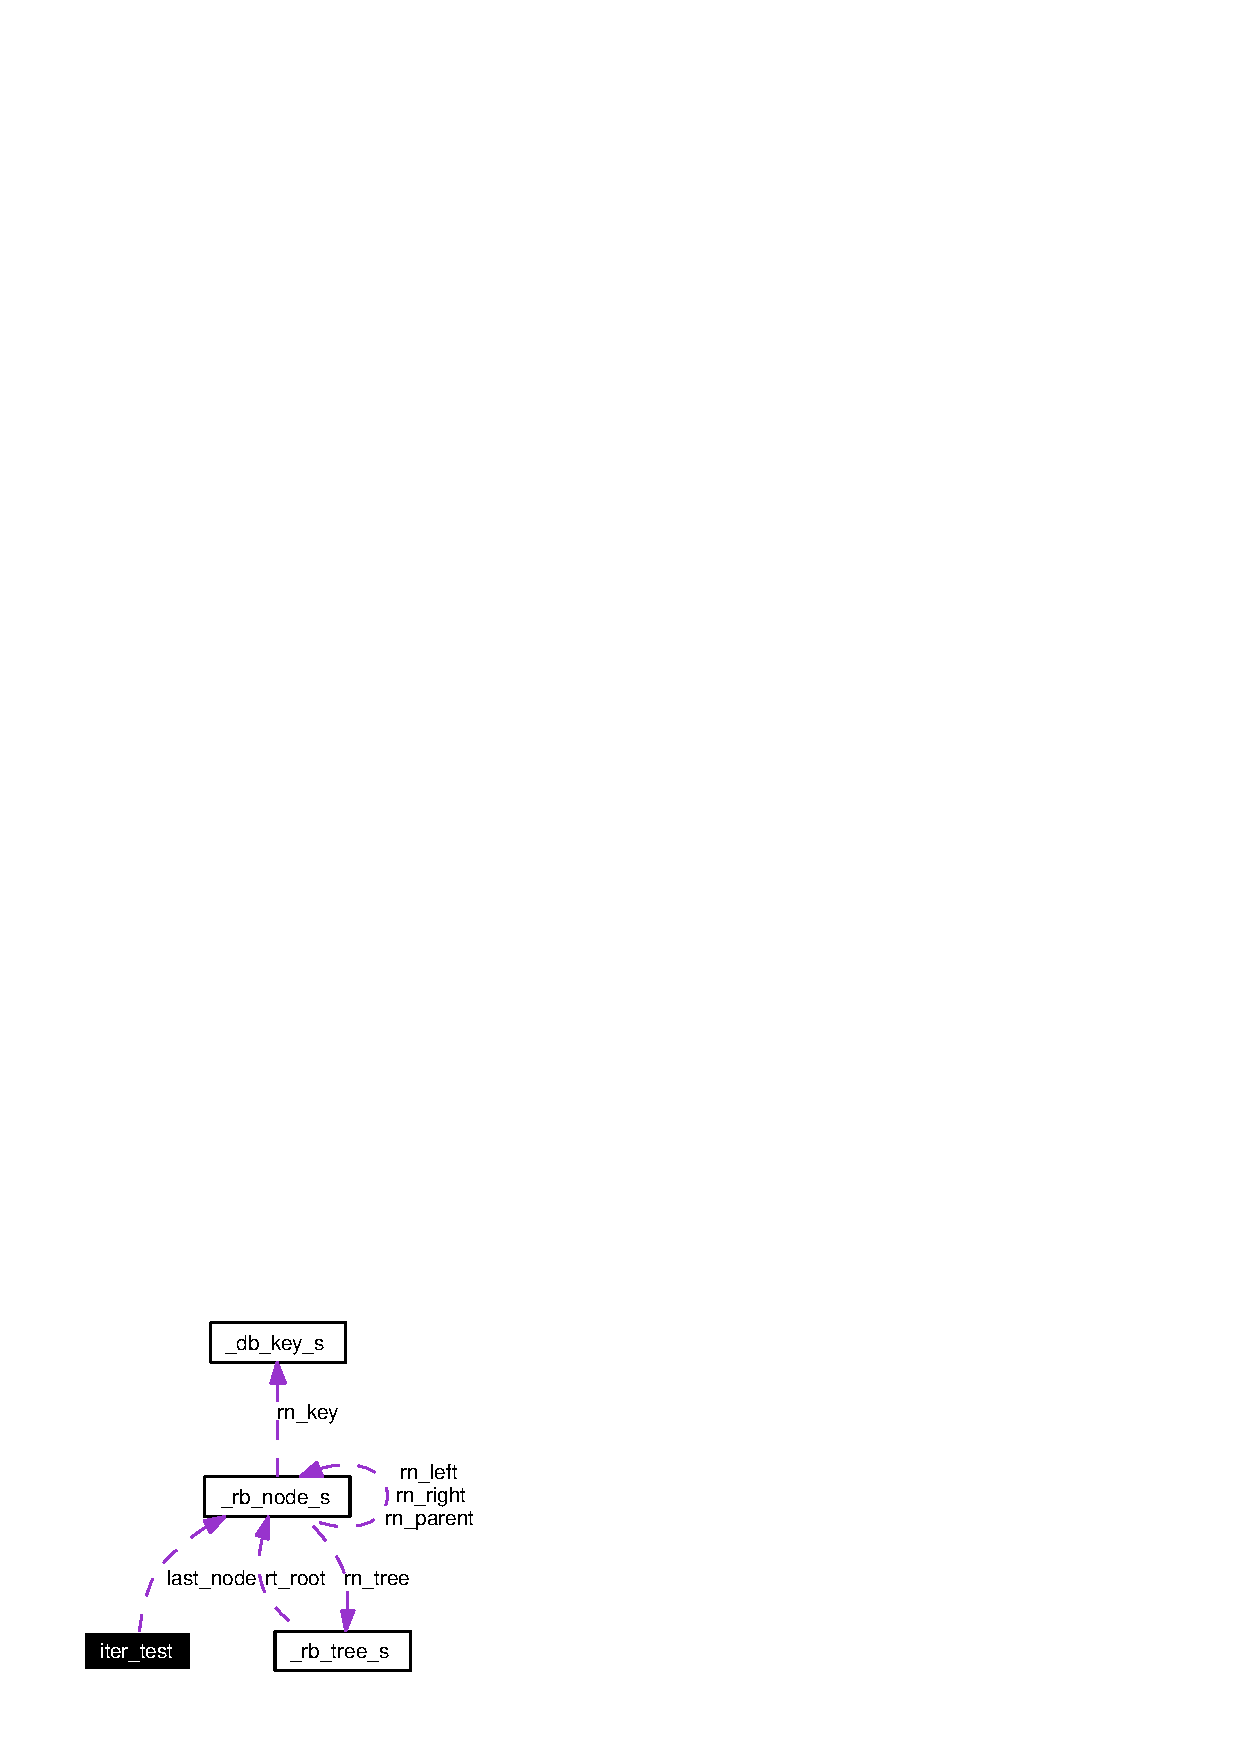
\includegraphics[width=116pt]{structiter__test__coll__graph}
\end{center}
\end{figure}


\subsection{Detailed Description}




Definition at line 260 of file t\_\-redblack.c.\subsection*{Data Fields}
\begin{CompactItemize}
\item 
unsigned long \hyperlink{structiter__test_o0}{visited}
\item 
int \hyperlink{structiter__test_o1}{stop\_\-node}
\item 
\hyperlink{struct__rb__node__s}{rb\_\-node\_\-t} $\ast$ \hyperlink{structiter__test_o2}{last\_\-node}
\item 
int \hyperlink{structiter__test_o3}{idx}
\item 
int \hyperlink{structiter__test_o4}{order} \mbox{[}RBT\_\-ELEM\_\-CNT\mbox{]}
\end{CompactItemize}


\subsection{Field Documentation}
\hypertarget{structiter__test_o3}{
\index{iter_test@{iter\_\-test}!idx@{idx}}
\index{idx@{idx}!iter_test@{iter\_\-test}}
\subsubsection[idx]{\setlength{\rightskip}{0pt plus 5cm}int \hyperlink{structiter__test_o3}{iter\_\-test::idx}}}
\label{structiter__test_o3}




Definition at line 264 of file t\_\-redblack.c.

Referenced by main(), and t\_\-iter().\hypertarget{structiter__test_o2}{
\index{iter_test@{iter\_\-test}!last_node@{last\_\-node}}
\index{last_node@{last\_\-node}!iter_test@{iter\_\-test}}
\subsubsection[last\_\-node]{\setlength{\rightskip}{0pt plus 5cm}\hyperlink{struct__rb__node__s}{rb\_\-node\_\-t}$\ast$ \hyperlink{structiter__test_o2}{iter\_\-test::last\_\-node}}}
\label{structiter__test_o2}




Definition at line 263 of file t\_\-redblack.c.

Referenced by main(), and t\_\-iter().\hypertarget{structiter__test_o4}{
\index{iter_test@{iter\_\-test}!order@{order}}
\index{order@{order}!iter_test@{iter\_\-test}}
\subsubsection[order]{\setlength{\rightskip}{0pt plus 5cm}int \hyperlink{structiter__test_o4}{iter\_\-test::order}\mbox{[}RBT\_\-ELEM\_\-CNT\mbox{]}}}
\label{structiter__test_o4}




Definition at line 265 of file t\_\-redblack.c.

Referenced by main(), and t\_\-iter().\hypertarget{structiter__test_o1}{
\index{iter_test@{iter\_\-test}!stop_node@{stop\_\-node}}
\index{stop_node@{stop\_\-node}!iter_test@{iter\_\-test}}
\subsubsection[stop\_\-node]{\setlength{\rightskip}{0pt plus 5cm}int \hyperlink{structiter__test_o1}{iter\_\-test::stop\_\-node}}}
\label{structiter__test_o1}




Definition at line 262 of file t\_\-redblack.c.

Referenced by main(), and t\_\-iter().\hypertarget{structiter__test_o0}{
\index{iter_test@{iter\_\-test}!visited@{visited}}
\index{visited@{visited}!iter_test@{iter\_\-test}}
\subsubsection[visited]{\setlength{\rightskip}{0pt plus 5cm}unsigned long \hyperlink{structiter__test_o0}{iter\_\-test::visited}}}
\label{structiter__test_o0}




Definition at line 261 of file t\_\-redblack.c.

Referenced by main(), and t\_\-iter().
\hypertarget{structmoves__s}{
\section{moves\_\-s Struct Reference}
\label{structmoves__s}\index{moves_s@{moves\_\-s}}
}
Collaboration diagram for moves\_\-s:\begin{figure}[H]
\begin{center}
\leavevmode
\includegraphics[width=54pt]{structmoves__s__coll__graph}
\end{center}
\end{figure}


\subsection{Detailed Description}




Definition at line 123 of file t\_\-hashtab.c.\subsection*{Data Fields}
\begin{CompactItemize}
\item 
int \hyperlink{structmoves__s_o0}{elem}
\item 
\hyperlink{struct__db__key__s}{db\_\-key\_\-t} \hyperlink{structmoves__s_o1}{key}
\end{CompactItemize}


\subsection{Field Documentation}
\hypertarget{structmoves__s_o0}{
\index{moves_s@{moves\_\-s}!elem@{elem}}
\index{elem@{elem}!moves_s@{moves\_\-s}}
\subsubsection[elem]{\setlength{\rightskip}{0pt plus 5cm}int \hyperlink{structmoves__s_o0}{moves\_\-s::elem}}}
\label{structmoves__s_o0}




Definition at line 124 of file t\_\-hashtab.c.\hypertarget{structmoves__s_o1}{
\index{moves_s@{moves\_\-s}!key@{key}}
\index{key@{key}!moves_s@{moves\_\-s}}
\subsubsection[key]{\setlength{\rightskip}{0pt plus 5cm}\hyperlink{struct__db__key__s}{db\_\-key\_\-t} \hyperlink{structmoves__s_o1}{moves\_\-s::key}}}
\label{structmoves__s_o1}




Definition at line 125 of file t\_\-hashtab.c.
\hypertarget{structtdata__s}{
\section{tdata\_\-s Struct Reference}
\label{structtdata__s}\index{tdata_s@{tdata\_\-s}}
}


\subsection{Detailed Description}




Definition at line 32 of file t\_\-linklists.c.\subsection*{Data Fields}
\begin{CompactItemize}
\item 
\hyperlink{group__dbprim__link_ga4}{link\_\-loc\_\-t} \hyperlink{structtdata__s_o0}{loc}
\item 
int \hyperlink{structtdata__s_o1}{elem}
\end{CompactItemize}


\subsection{Field Documentation}
\hypertarget{structtdata__s_o1}{
\index{tdata_s@{tdata\_\-s}!elem@{elem}}
\index{elem@{elem}!tdata_s@{tdata\_\-s}}
\subsubsection[elem]{\setlength{\rightskip}{0pt plus 5cm}int \hyperlink{structtdata__s_o1}{tdata\_\-s::elem}}}
\label{structtdata__s_o1}




Definition at line 34 of file t\_\-linklists.c.\hypertarget{structtdata__s_o0}{
\index{tdata_s@{tdata\_\-s}!loc@{loc}}
\index{loc@{loc}!tdata_s@{tdata\_\-s}}
\subsubsection[loc]{\setlength{\rightskip}{0pt plus 5cm}\hyperlink{group__dbprim__link_ga4}{link\_\-loc\_\-t} \hyperlink{structtdata__s_o0}{tdata\_\-s::loc}}}
\label{structtdata__s_o0}




Definition at line 33 of file t\_\-linklists.c.
\hypertarget{structtmove__s}{
\section{tmove\_\-s Struct Reference}
\label{structtmove__s}\index{tmove_s@{tmove\_\-s}}
}


\subsection{Detailed Description}




Definition at line 48 of file t\_\-linklists.c.\subsection*{Data Fields}
\begin{CompactItemize}
\item 
int \hyperlink{structtmove__s_o0}{elem}
\item 
\hyperlink{group__dbprim__link_ga4}{link\_\-loc\_\-t} \hyperlink{structtmove__s_o1}{loc}
\item 
int \hyperlink{structtmove__s_o2}{elem2}
\end{CompactItemize}


\subsection{Field Documentation}
\hypertarget{structtmove__s_o0}{
\index{tmove_s@{tmove\_\-s}!elem@{elem}}
\index{elem@{elem}!tmove_s@{tmove\_\-s}}
\subsubsection[elem]{\setlength{\rightskip}{0pt plus 5cm}int \hyperlink{structtmove__s_o0}{tmove\_\-s::elem}}}
\label{structtmove__s_o0}




Definition at line 49 of file t\_\-linklists.c.\hypertarget{structtmove__s_o2}{
\index{tmove_s@{tmove\_\-s}!elem2@{elem2}}
\index{elem2@{elem2}!tmove_s@{tmove\_\-s}}
\subsubsection[elem2]{\setlength{\rightskip}{0pt plus 5cm}int \hyperlink{structtmove__s_o2}{tmove\_\-s::elem2}}}
\label{structtmove__s_o2}




Definition at line 51 of file t\_\-linklists.c.\hypertarget{structtmove__s_o1}{
\index{tmove_s@{tmove\_\-s}!loc@{loc}}
\index{loc@{loc}!tmove_s@{tmove\_\-s}}
\subsubsection[loc]{\setlength{\rightskip}{0pt plus 5cm}\hyperlink{group__dbprim__link_ga4}{link\_\-loc\_\-t} \hyperlink{structtmove__s_o1}{tmove\_\-s::loc}}}
\label{structtmove__s_o1}




Definition at line 50 of file t\_\-linklists.c.
\chapter{@PACKAGE\_\-NAME@ File Documentation}
\input{__hash__prime_8c}
\include{__rb__locate_8c}
\include{__rb__rotate_8c}
\hypertarget{__smat__comp_8c}{
\section{\_\-smat\_\-comp.c File Reference}
\label{__smat__comp_8c}\index{_smat_comp.c@{\_\-smat\_\-comp.c}}
}


\subsection{Detailed Description}
\begin{Desc}
\item[For internal use only.]
This file contains the implementation of the \hyperlink{group__dbprim__smat_ga10}{\_\-smat\_\-comp()} function, the comparison callback used by sparse matrices.\end{Desc}


Definition in file \hyperlink{__smat__comp_8c-source}{\_\-smat\_\-comp.c}.

{\tt \#include \char`\"{}dbprim.h\char`\"{}}\par
{\tt \#include \char`\"{}dbprim\_\-int.h\char`\"{}}\par


Include dependency graph for \_\-smat\_\-comp.c:\begin{figure}[H]
\begin{center}
\leavevmode
\includegraphics[width=199pt]{__smat__comp_8c__incl}
\end{center}
\end{figure}
\subsection*{Functions}
\begin{CompactItemize}
\item 
unsigned long \hyperlink{group__dbprim__smat_ga10}{\_\-smat\_\-comp} (\hyperlink{struct__hash__table__s}{hash\_\-table\_\-t} $\ast$table, \hyperlink{struct__db__key__s}{db\_\-key\_\-t} $\ast$key1, \hyperlink{struct__db__key__s}{db\_\-key\_\-t} $\ast$key2)
\begin{CompactList}\small\item\em Sparse matrix comparison function. \item\end{CompactList}\end{CompactItemize}

\include{__smat__resize_8c}
\include{dbprim_8h}
\include{dbprim__int_8h}
\include{hash__fnv1_8c}
\include{hash__fnv1a_8c}
\include{he__init_8c}
\include{ht__add_8c}
\include{ht__find_8c}
\include{ht__flush_8c}
\include{ht__free_8c}
\include{ht__init_8c}
\include{ht__iter_8c}
\include{ht__move_8c}
\include{ht__remove_8c}
\include{ht__resize_8c}
\include{le__init_8c}
\include{ll__add_8c}
\include{ll__find_8c}
\include{ll__flush_8c}
\include{ll__init_8c}
\include{ll__iter_8c}
\include{ll__move_8c}
\include{ll__remove_8c}
\include{rn__init_8c}
\include{rt__add_8c}
\include{rt__find_8c}
\include{rt__flush_8c}
\include{rt__init_8c}
\include{rt__iter_8c}
\include{rt__move_8c}
\include{rt__next_8c}
\include{rt__remove_8c}
\include{sh__find_8c}
\hypertarget{sh__flush_8c}{
\section{sh\_\-flush.c File Reference}
\label{sh__flush_8c}\index{sh_flush.c@{sh\_\-flush.c}}
}


\subsection{Detailed Description}
\begin{Desc}
\item[For internal use only.]
This file contains the implementation of the \hyperlink{dbprim_8h_a178}{sh\_\-flush()} function, used to release all entries in a sparse matrix linked list.\end{Desc}


Definition in file \hyperlink{sh__flush_8c-source}{sh\_\-flush.c}.

{\tt \#include \char`\"{}dbprim.h\char`\"{}}\par
{\tt \#include \char`\"{}dbprim\_\-int.h\char`\"{}}\par


Include dependency graph for sh\_\-flush.c:\begin{figure}[H]
\begin{center}
\leavevmode
\includegraphics[width=188pt]{sh__flush_8c__incl}
\end{center}
\end{figure}
\subsection*{Data Structures}
\begin{CompactItemize}
\item 
struct \hyperlink{struct__sh__flush__s}{\_\-sh\_\-flush\_\-s}
\begin{CompactList}\small\item\em Sparse matrix flush function shim structure. \item\end{CompactList}\end{CompactItemize}
\subsection*{Functions}
\begin{CompactItemize}
\item 
static unsigned long \hyperlink{group__dbprim__smat_ga28}{\_\-sh\_\-flush\_\-iter} (\hyperlink{struct__link__head__s}{link\_\-head\_\-t} $\ast$head, \hyperlink{struct__link__elem__s}{link\_\-elem\_\-t} $\ast$elem, void $\ast$extra)
\begin{CompactList}\small\item\em Sparse matrix linked list flush callback. \item\end{CompactList}\item 
unsigned long \hyperlink{sh__flush_8c_a1}{sh\_\-flush} (\hyperlink{struct__smat__head__s}{smat\_\-head\_\-t} $\ast$head, \hyperlink{group__dbprim__smat_ga4}{smat\_\-iter\_\-t} flush\_\-func, void $\ast$extra)
\begin{CompactList}\small\item\em Flush a row or column of a sparse matrix. \item\end{CompactList}\end{CompactItemize}


\subsection{Function Documentation}
\hypertarget{sh__flush_8c_a1}{
\index{sh_flush.c@{sh\_\-flush.c}!sh_flush@{sh\_\-flush}}
\index{sh_flush@{sh\_\-flush}!sh_flush.c@{sh\_\-flush.c}}
\subsubsection[sh\_\-flush]{\setlength{\rightskip}{0pt plus 5cm}unsigned long sh\_\-flush (\hyperlink{struct__smat__head__s}{smat\_\-head\_\-t} $\ast$ {\em head}, \hyperlink{group__dbprim__smat_ga4}{smat\_\-iter\_\-t} {\em flush\_\-func}, void $\ast$ {\em extra})}}
\label{sh__flush_8c_a1}


ingroup dbprim\_\-smat

This function flushes a sparse matrix row or column--that is, it removes each element from that row or column. If a {\tt flush\_\-func} is specified, it will be called on the entry after it has been removed from the row or column, and may safely call {\tt free()}.

\begin{Desc}
\item[Parameters:]
\begin{description}
\item[\mbox{$\leftarrow$} {\em head}]A pointer to a \hyperlink{group__dbprim__smat_ga1}{smat\_\-head\_\-t}. \item[\mbox{$\leftarrow$} {\em flush\_\-func}]A pointer to a callback function used to perform user-specifed actions on an entry after removing it from the row or column. May be {\tt NULL}. See the documentation for \hyperlink{group__dbprim__smat_ga4}{smat\_\-iter\_\-t} for more information. \item[\mbox{$\leftarrow$} {\em extra}]A {\tt void} pointer that will be passed to {\tt flush\_\-func}.\end{description}
\end{Desc}
\begin{Desc}
\item[Return values:]
\begin{description}
\item[{\em DB\_\-ERR\_\-BADARGS}]An argument was invalid.\end{description}
\end{Desc}


Definition at line 90 of file sh\_\-flush.c.

References \_\-sh\_\-flush\_\-iter(), ll\_\-flush(), \_\-sh\_\-flush\_\-s::sf\_\-elem, \_\-sh\_\-flush\_\-s::sf\_\-extra, \_\-sh\_\-flush\_\-s::sf\_\-flush, \_\-sh\_\-flush\_\-s::sf\_\-table, \_\-smat\_\-head\_\-s::sh\_\-elem, \_\-smat\_\-head\_\-s::sh\_\-head, \_\-smat\_\-head\_\-s::sh\_\-table, and sh\_\-verify.

Here is the call graph for this function:\begin{figure}[H]
\begin{center}
\leavevmode
\includegraphics[width=315pt]{sh__flush_8c_a1_cgraph}
\end{center}
\end{figure}

\include{sh__init_8c}
\include{sh__iter_8c}
\include{sh__move_8c}
\include{smat__freelist_8c}
\include{st__add_8c}
\include{st__find_8c}
\include{st__flush_8c}
\include{st__free_8c}
\include{st__init_8c}
\include{st__iter_8c}
\include{st__remove_8c}
\include{st__resize_8c}
\hypertarget{t__hashtab_8c}{
\section{t\_\-hashtab.c File Reference}
\label{t__hashtab_8c}\index{t_hashtab.c@{t\_\-hashtab.c}}
}


{\tt \#include $<$stdio.h$>$}\par
{\tt \#include $<$stdlib.h$>$}\par
{\tt \#include $<$string.h$>$}\par
{\tt \#include $<$time.h$>$}\par
{\tt \#include \char`\"{}test-harness.h\char`\"{}}\par
{\tt \#include \char`\"{}dbprim.h\char`\"{}}\par
{\tt \#include \char`\"{}dbprim\_\-int.h\char`\"{}}\par


Include dependency graph for t\_\-hashtab.c:\begin{figure}[H]
\begin{center}
\leavevmode
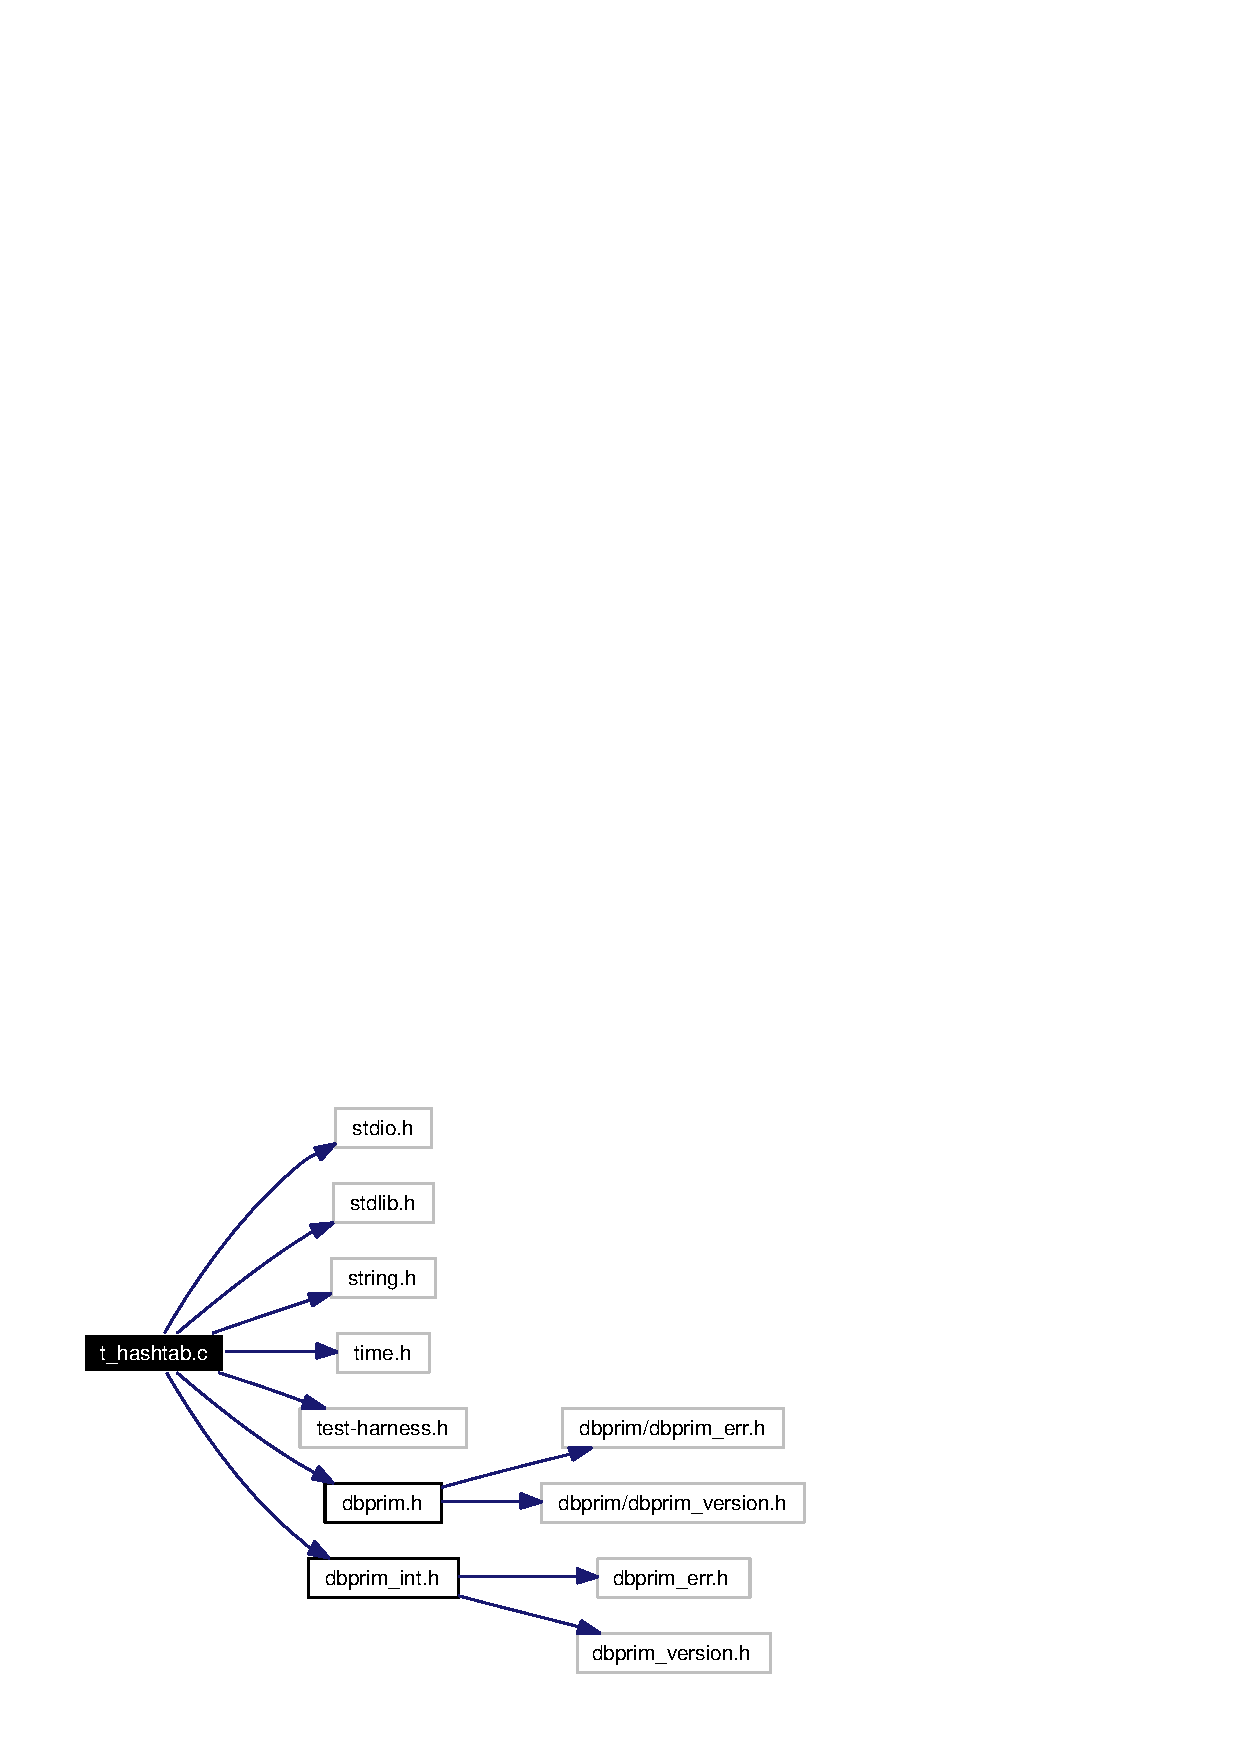
\includegraphics[width=195pt]{t__hashtab_8c__incl}
\end{center}
\end{figure}
\subsection*{Data Structures}
\begin{CompactItemize}
\item 
struct \hyperlink{structmoves__s}{moves\_\-s}
\item 
struct \hyperlink{structiter__s}{iter\_\-s}
\end{CompactItemize}
\subsection*{Defines}
\begin{CompactItemize}
\item 
\#define \hyperlink{t__hashtab_8c_a0}{FLUSH\_\-THRESHOLD}
\item 
\#define \hyperlink{t__hashtab_8c_a1}{\_\-hw}(n, m, s)
\item 
\#define \hyperlink{t__hashtab_8c_a2}{RSF\_\-INHIBIT}
\item 
\#define \hyperlink{t__hashtab_8c_a3}{RSF\_\-RESIZE}
\item 
\#define \hyperlink{t__hashtab_8c_a4}{HASH\_\-ENT\_\-CNT}
\item 
\#define \hyperlink{t__hashtab_8c_a5}{HASH\_\-MOVE\_\-CNT}
\item 
\#define \hyperlink{t__hashtab_8c_a6}{HASH\_\-REMOVE\_\-CNT}
\item 
\#define \hyperlink{t__hashtab_8c_a7}{VISIT\_\-INIT}
\end{CompactItemize}
\subsection*{Functions}
\begin{CompactItemize}
\item 
static unsigned long \hyperlink{t__hashtab_8c_a14}{hamming} (unsigned long bits)
\item 
static unsigned long \hyperlink{t__hashtab_8c_a15}{t\_\-hash} (\hyperlink{struct__hash__table__s}{hash\_\-table\_\-t} $\ast$tab, \hyperlink{struct__db__key__s}{db\_\-key\_\-t} $\ast$key)
\item 
static unsigned long \hyperlink{t__hashtab_8c_a16}{t\_\-comp} (\hyperlink{struct__hash__table__s}{hash\_\-table\_\-t} $\ast$tab, \hyperlink{struct__db__key__s}{db\_\-key\_\-t} $\ast$key1, \hyperlink{struct__db__key__s}{db\_\-key\_\-t} $\ast$key2)
\item 
static unsigned long \hyperlink{t__hashtab_8c_a17}{t\_\-resize} (\hyperlink{struct__hash__table__s}{hash\_\-table\_\-t} $\ast$tab, unsigned long new)
\item 
static unsigned long \hyperlink{t__hashtab_8c_a18}{t\_\-iter} (\hyperlink{struct__hash__table__s}{hash\_\-table\_\-t} $\ast$tab, \hyperlink{struct__hash__entry__s}{hash\_\-entry\_\-t} $\ast$ent, struct \hyperlink{structiter__s}{iter\_\-s} $\ast$iter)
\item 
int \hyperlink{t__hashtab_8c_a19}{main} (int argc, char $\ast$$\ast$argv)
\end{CompactItemize}
\subsection*{Variables}
\begin{CompactItemize}
\item 
static unsigned int \hyperlink{t__hashtab_8c_a8}{rsize\_\-flags}
\item 
static unsigned long \hyperlink{t__hashtab_8c_a9}{rsize\_\-new}
\item 
static unsigned long \hyperlink{t__hashtab_8c_a10}{rsize\_\-err}
\item 
static \hyperlink{struct__db__key__s}{db\_\-key\_\-t} \hyperlink{t__hashtab_8c_a11}{keys} \mbox{[}$\,$\mbox{]}
\item 
static struct \hyperlink{structmoves__s}{moves\_\-s} \hyperlink{t__hashtab_8c_a12}{moves} \mbox{[}$\,$\mbox{]}
\item 
static int \hyperlink{t__hashtab_8c_a13}{removes} \mbox{[}$\,$\mbox{]}
\end{CompactItemize}


\subsection{Define Documentation}
\hypertarget{t__hashtab_8c_a1}{
\index{t_hashtab.c@{t\_\-hashtab.c}!_hw@{\_\-hw}}
\index{_hw@{\_\-hw}!t_hashtab.c@{t\_\-hashtab.c}}
\subsubsection[\_\-hw]{\setlength{\rightskip}{0pt plus 5cm}\#define \_\-hw(n, m, s)}}
\label{t__hashtab_8c_a1}




Referenced by hamming().\hypertarget{t__hashtab_8c_a0}{
\index{t_hashtab.c@{t\_\-hashtab.c}!FLUSH_THRESHOLD@{FLUSH\_\-THRESHOLD}}
\index{FLUSH_THRESHOLD@{FLUSH\_\-THRESHOLD}!t_hashtab.c@{t\_\-hashtab.c}}
\subsubsection[FLUSH\_\-THRESHOLD]{\setlength{\rightskip}{0pt plus 5cm}\#define FLUSH\_\-THRESHOLD}}
\label{t__hashtab_8c_a0}




Definition at line 35 of file t\_\-hashtab.c.

Referenced by main().\hypertarget{t__hashtab_8c_a4}{
\index{t_hashtab.c@{t\_\-hashtab.c}!HASH_ENT_CNT@{HASH\_\-ENT\_\-CNT}}
\index{HASH_ENT_CNT@{HASH\_\-ENT\_\-CNT}!t_hashtab.c@{t\_\-hashtab.c}}
\subsubsection[HASH\_\-ENT\_\-CNT]{\setlength{\rightskip}{0pt plus 5cm}\#define HASH\_\-ENT\_\-CNT}}
\label{t__hashtab_8c_a4}




Definition at line 121 of file t\_\-hashtab.c.

Referenced by main().\hypertarget{t__hashtab_8c_a5}{
\index{t_hashtab.c@{t\_\-hashtab.c}!HASH_MOVE_CNT@{HASH\_\-MOVE\_\-CNT}}
\index{HASH_MOVE_CNT@{HASH\_\-MOVE\_\-CNT}!t_hashtab.c@{t\_\-hashtab.c}}
\subsubsection[HASH\_\-MOVE\_\-CNT]{\setlength{\rightskip}{0pt plus 5cm}\#define HASH\_\-MOVE\_\-CNT}}
\label{t__hashtab_8c_a5}




Definition at line 139 of file t\_\-hashtab.c.

Referenced by main().\hypertarget{t__hashtab_8c_a6}{
\index{t_hashtab.c@{t\_\-hashtab.c}!HASH_REMOVE_CNT@{HASH\_\-REMOVE\_\-CNT}}
\index{HASH_REMOVE_CNT@{HASH\_\-REMOVE\_\-CNT}!t_hashtab.c@{t\_\-hashtab.c}}
\subsubsection[HASH\_\-REMOVE\_\-CNT]{\setlength{\rightskip}{0pt plus 5cm}\#define HASH\_\-REMOVE\_\-CNT}}
\label{t__hashtab_8c_a6}




Definition at line 143 of file t\_\-hashtab.c.

Referenced by main().\hypertarget{t__hashtab_8c_a2}{
\index{t_hashtab.c@{t\_\-hashtab.c}!RSF_INHIBIT@{RSF\_\-INHIBIT}}
\index{RSF_INHIBIT@{RSF\_\-INHIBIT}!t_hashtab.c@{t\_\-hashtab.c}}
\subsubsection[RSF\_\-INHIBIT]{\setlength{\rightskip}{0pt plus 5cm}\#define RSF\_\-INHIBIT}}
\label{t__hashtab_8c_a2}




Definition at line 86 of file t\_\-hashtab.c.

Referenced by main(), and t\_\-resize().\hypertarget{t__hashtab_8c_a3}{
\index{t_hashtab.c@{t\_\-hashtab.c}!RSF_RESIZE@{RSF\_\-RESIZE}}
\index{RSF_RESIZE@{RSF\_\-RESIZE}!t_hashtab.c@{t\_\-hashtab.c}}
\subsubsection[RSF\_\-RESIZE]{\setlength{\rightskip}{0pt plus 5cm}\#define RSF\_\-RESIZE}}
\label{t__hashtab_8c_a3}




Definition at line 87 of file t\_\-hashtab.c.

Referenced by main(), and t\_\-resize().\hypertarget{t__hashtab_8c_a7}{
\index{t_hashtab.c@{t\_\-hashtab.c}!VISIT_INIT@{VISIT\_\-INIT}}
\index{VISIT_INIT@{VISIT\_\-INIT}!t_hashtab.c@{t\_\-hashtab.c}}
\subsubsection[VISIT\_\-INIT]{\setlength{\rightskip}{0pt plus 5cm}\#define VISIT\_\-INIT}}
\label{t__hashtab_8c_a7}




Definition at line 151 of file t\_\-hashtab.c.

Referenced by main().

\subsection{Function Documentation}
\hypertarget{t__hashtab_8c_a14}{
\index{t_hashtab.c@{t\_\-hashtab.c}!hamming@{hamming}}
\index{hamming@{hamming}!t_hashtab.c@{t\_\-hashtab.c}}
\subsubsection[hamming]{\setlength{\rightskip}{0pt plus 5cm}static unsigned long hamming (unsigned long {\em bits})\hspace{0.3cm}{\tt  \mbox{[}static\mbox{]}}}}
\label{t__hashtab_8c_a14}




Definition at line 39 of file t\_\-hashtab.c.

References \_\-hw.

Referenced by main().\hypertarget{t__hashtab_8c_a19}{
\index{t_hashtab.c@{t\_\-hashtab.c}!main@{main}}
\index{main@{main}!t_hashtab.c@{t\_\-hashtab.c}}
\subsubsection[main]{\setlength{\rightskip}{0pt plus 5cm}int main (int {\em argc}, char $\ast$$\ast$ {\em argv})}}
\label{t__hashtab_8c_a19}




Definition at line 170 of file t\_\-hashtab.c.

References iter\_\-s::elem, FLUSH\_\-THRESHOLD, hamming(), HASH\_\-ENT\_\-CNT, HASH\_\-FLAG\_\-AUTOGROW, HASH\_\-FLAG\_\-AUTOSHRINK, HASH\_\-MOVE\_\-CNT, HASH\_\-REMOVE\_\-CNT, he\_\-init(), ht\_\-add(), ht\_\-count, ht\_\-find(), ht\_\-flags, ht\_\-flush(), ht\_\-free(), ht\_\-init(), ht\_\-iter(), ht\_\-modulus, ht\_\-move(), ht\_\-remove(), ht\_\-resize(), \_\-hash\_\-table\_\-s::ht\_\-table, moves, removes, RSF\_\-INHIBIT, RSF\_\-RESIZE, rsize\_\-err, rsize\_\-flags, rsize\_\-new, t\_\-comp(), t\_\-hash(), t\_\-iter(), t\_\-resize(), VISIT\_\-INIT, and iter\_\-s::visited.

Here is the call graph for this function:\begin{figure}[H]
\begin{center}
\leavevmode
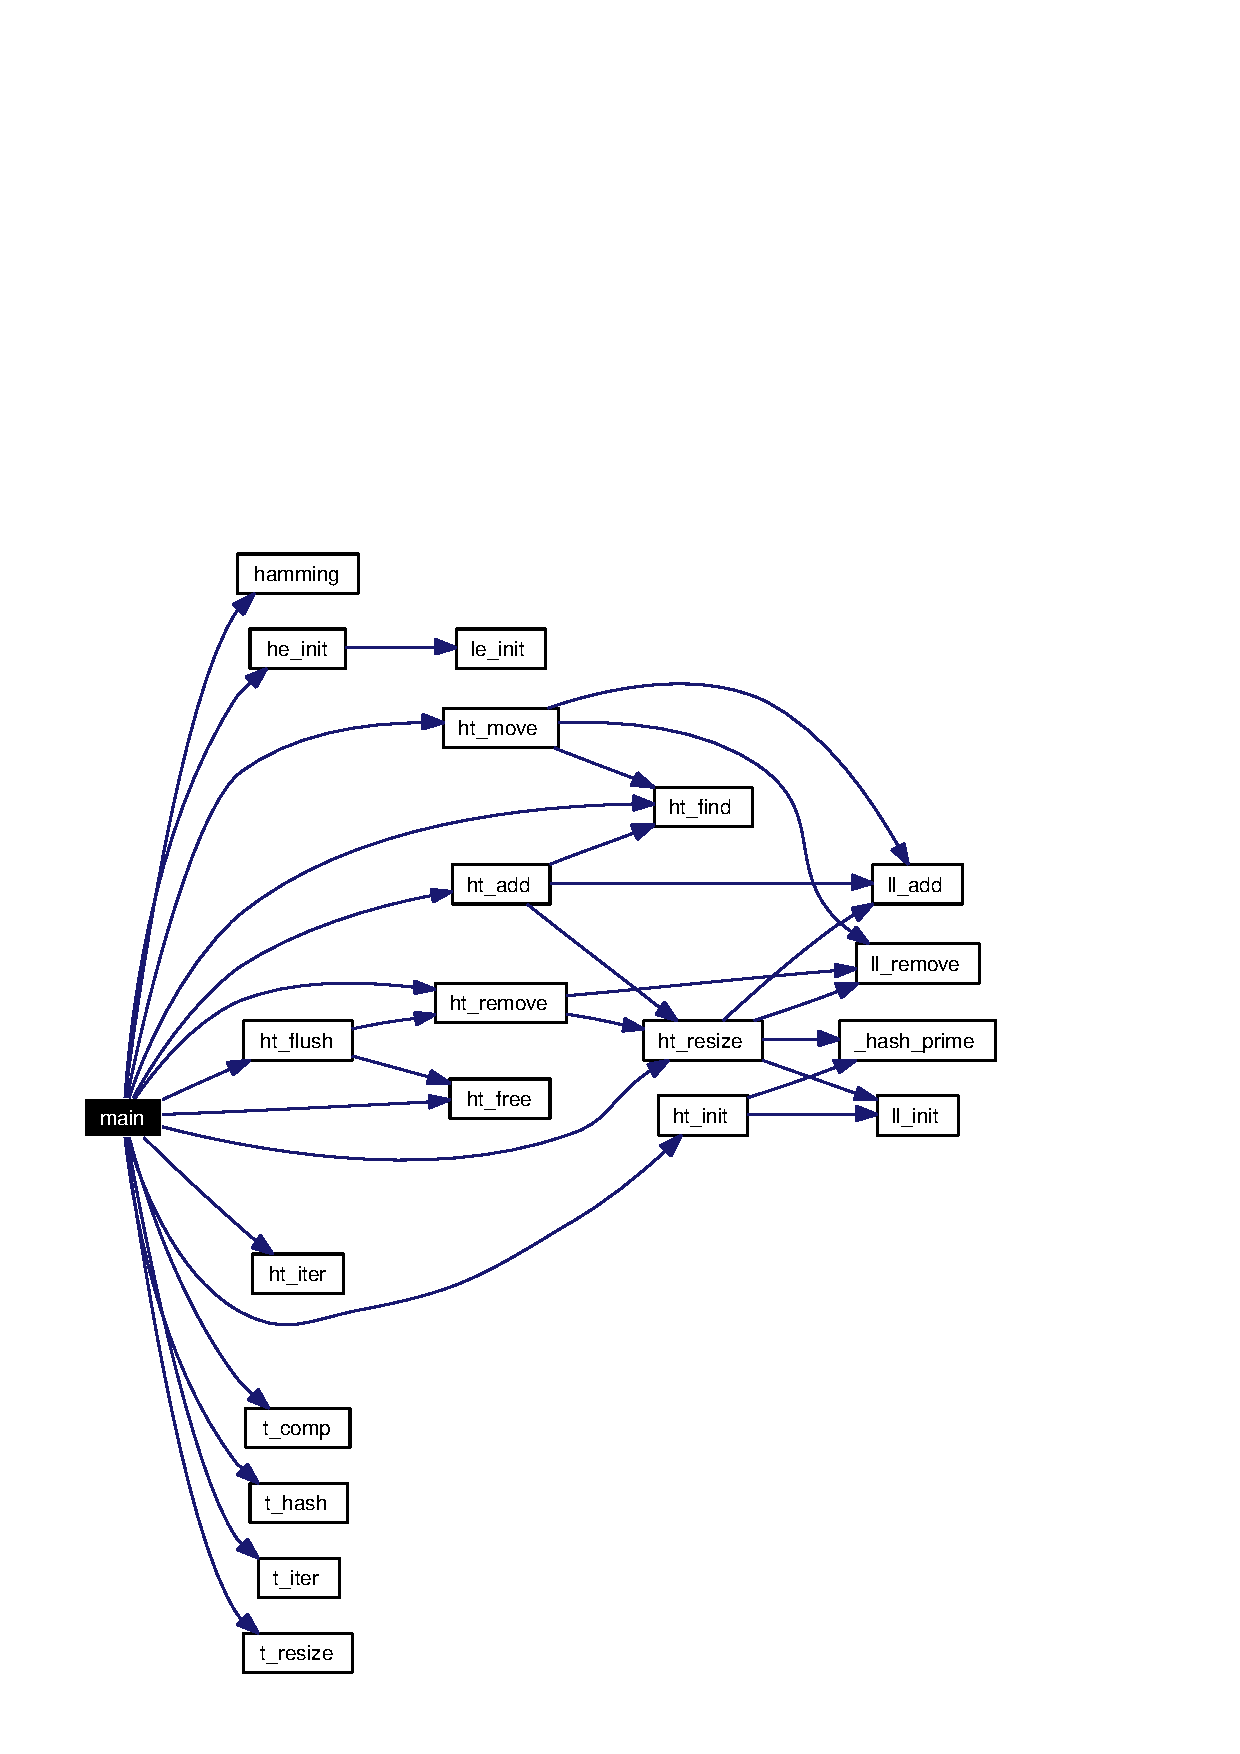
\includegraphics[width=241pt]{t__hashtab_8c_a19_cgraph}
\end{center}
\end{figure}
\hypertarget{t__hashtab_8c_a16}{
\index{t_hashtab.c@{t\_\-hashtab.c}!t_comp@{t\_\-comp}}
\index{t_comp@{t\_\-comp}!t_hashtab.c@{t\_\-hashtab.c}}
\subsubsection[t\_\-comp]{\setlength{\rightskip}{0pt plus 5cm}static unsigned long t\_\-comp (\hyperlink{struct__hash__table__s}{hash\_\-table\_\-t} $\ast$ {\em tab}, \hyperlink{struct__db__key__s}{db\_\-key\_\-t} $\ast$ {\em key1}, \hyperlink{struct__db__key__s}{db\_\-key\_\-t} $\ast$ {\em key2})\hspace{0.3cm}{\tt  \mbox{[}static\mbox{]}}}}
\label{t__hashtab_8c_a16}




Definition at line 70 of file t\_\-hashtab.c.

References dk\_\-key, and dk\_\-len.

Referenced by main().\hypertarget{t__hashtab_8c_a15}{
\index{t_hashtab.c@{t\_\-hashtab.c}!t_hash@{t\_\-hash}}
\index{t_hash@{t\_\-hash}!t_hashtab.c@{t\_\-hashtab.c}}
\subsubsection[t\_\-hash]{\setlength{\rightskip}{0pt plus 5cm}static unsigned long t\_\-hash (\hyperlink{struct__hash__table__s}{hash\_\-table\_\-t} $\ast$ {\em tab}, \hyperlink{struct__db__key__s}{db\_\-key\_\-t} $\ast$ {\em key})\hspace{0.3cm}{\tt  \mbox{[}static\mbox{]}}}}
\label{t__hashtab_8c_a15}




Definition at line 53 of file t\_\-hashtab.c.

References dk\_\-key, and dk\_\-len.

Referenced by main().\hypertarget{t__hashtab_8c_a18}{
\index{t_hashtab.c@{t\_\-hashtab.c}!t_iter@{t\_\-iter}}
\index{t_iter@{t\_\-iter}!t_hashtab.c@{t\_\-hashtab.c}}
\subsubsection[t\_\-iter]{\setlength{\rightskip}{0pt plus 5cm}static unsigned long t\_\-iter (\hyperlink{struct__hash__table__s}{hash\_\-table\_\-t} $\ast$ {\em tab}, \hyperlink{struct__hash__entry__s}{hash\_\-entry\_\-t} $\ast$ {\em ent}, struct \hyperlink{structiter__s}{iter\_\-s} $\ast$ {\em iter})\hspace{0.3cm}{\tt  \mbox{[}static\mbox{]}}}}
\label{t__hashtab_8c_a18}




Definition at line 154 of file t\_\-hashtab.c.

References iter\_\-s::elem, iter\_\-s::err, he\_\-value, and iter\_\-s::visited.

Referenced by main().\hypertarget{t__hashtab_8c_a17}{
\index{t_hashtab.c@{t\_\-hashtab.c}!t_resize@{t\_\-resize}}
\index{t_resize@{t\_\-resize}!t_hashtab.c@{t\_\-hashtab.c}}
\subsubsection[t\_\-resize]{\setlength{\rightskip}{0pt plus 5cm}static unsigned long t\_\-resize (\hyperlink{struct__hash__table__s}{hash\_\-table\_\-t} $\ast$ {\em tab}, unsigned long {\em new})\hspace{0.3cm}{\tt  \mbox{[}static\mbox{]}}}}
\label{t__hashtab_8c_a17}




Definition at line 94 of file t\_\-hashtab.c.

References RSF\_\-INHIBIT, RSF\_\-RESIZE, rsize\_\-err, rsize\_\-flags, and rsize\_\-new.

Referenced by main().

\subsection{Variable Documentation}
\hypertarget{t__hashtab_8c_a11}{
\index{t_hashtab.c@{t\_\-hashtab.c}!keys@{keys}}
\index{keys@{keys}!t_hashtab.c@{t\_\-hashtab.c}}
\subsubsection[keys]{\setlength{\rightskip}{0pt plus 5cm}\hyperlink{struct__db__key__s}{db\_\-key\_\-t} \hyperlink{t__hashtab_8c_a11}{keys}\mbox{[}$\,$\mbox{]}\hspace{0.3cm}{\tt  \mbox{[}static\mbox{]}}}}
\label{t__hashtab_8c_a11}




Definition at line 103 of file t\_\-hashtab.c.\hypertarget{t__hashtab_8c_a12}{
\index{t_hashtab.c@{t\_\-hashtab.c}!moves@{moves}}
\index{moves@{moves}!t_hashtab.c@{t\_\-hashtab.c}}
\subsubsection[moves]{\setlength{\rightskip}{0pt plus 5cm}struct \hyperlink{structmoves__s}{moves\_\-s}  \hyperlink{t__hashtab_8c_a12}{moves}\mbox{[}$\,$\mbox{]}\hspace{0.3cm}{\tt  \mbox{[}static\mbox{]}}}}
\label{t__hashtab_8c_a12}




Referenced by main().\hypertarget{t__hashtab_8c_a13}{
\index{t_hashtab.c@{t\_\-hashtab.c}!removes@{removes}}
\index{removes@{removes}!t_hashtab.c@{t\_\-hashtab.c}}
\subsubsection[removes]{\setlength{\rightskip}{0pt plus 5cm}int \hyperlink{t__hashtab_8c_a13}{removes}\mbox{[}$\,$\mbox{]}\hspace{0.3cm}{\tt  \mbox{[}static\mbox{]}}}}
\label{t__hashtab_8c_a13}




Definition at line 141 of file t\_\-hashtab.c.

Referenced by main().\hypertarget{t__hashtab_8c_a10}{
\index{t_hashtab.c@{t\_\-hashtab.c}!rsize_err@{rsize\_\-err}}
\index{rsize_err@{rsize\_\-err}!t_hashtab.c@{t\_\-hashtab.c}}
\subsubsection[rsize\_\-err]{\setlength{\rightskip}{0pt plus 5cm}unsigned long \hyperlink{t__hashtab_8c_a10}{rsize\_\-err}\hspace{0.3cm}{\tt  \mbox{[}static\mbox{]}}}}
\label{t__hashtab_8c_a10}




Definition at line 90 of file t\_\-hashtab.c.

Referenced by main(), and t\_\-resize().\hypertarget{t__hashtab_8c_a8}{
\index{t_hashtab.c@{t\_\-hashtab.c}!rsize_flags@{rsize\_\-flags}}
\index{rsize_flags@{rsize\_\-flags}!t_hashtab.c@{t\_\-hashtab.c}}
\subsubsection[rsize\_\-flags]{\setlength{\rightskip}{0pt plus 5cm}unsigned int \hyperlink{t__hashtab_8c_a8}{rsize\_\-flags}\hspace{0.3cm}{\tt  \mbox{[}static\mbox{]}}}}
\label{t__hashtab_8c_a8}




Definition at line 84 of file t\_\-hashtab.c.

Referenced by main(), and t\_\-resize().\hypertarget{t__hashtab_8c_a9}{
\index{t_hashtab.c@{t\_\-hashtab.c}!rsize_new@{rsize\_\-new}}
\index{rsize_new@{rsize\_\-new}!t_hashtab.c@{t\_\-hashtab.c}}
\subsubsection[rsize\_\-new]{\setlength{\rightskip}{0pt plus 5cm}unsigned long \hyperlink{t__hashtab_8c_a9}{rsize\_\-new}\hspace{0.3cm}{\tt  \mbox{[}static\mbox{]}}}}
\label{t__hashtab_8c_a9}




Definition at line 89 of file t\_\-hashtab.c.

Referenced by main(), and t\_\-resize().
\hypertarget{t__linklists_8c}{
\section{t\_\-linklists.c File Reference}
\label{t__linklists_8c}\index{t_linklists.c@{t\_\-linklists.c}}
}


{\tt \#include $<$stdio.h$>$}\par
{\tt \#include \char`\"{}test-harness.h\char`\"{}}\par
{\tt \#include \char`\"{}dbprim.h\char`\"{}}\par
{\tt \#include \char`\"{}dbprim\_\-int.h\char`\"{}}\par


Include dependency graph for t\_\-linklists.c:\begin{figure}[H]
\begin{center}
\leavevmode
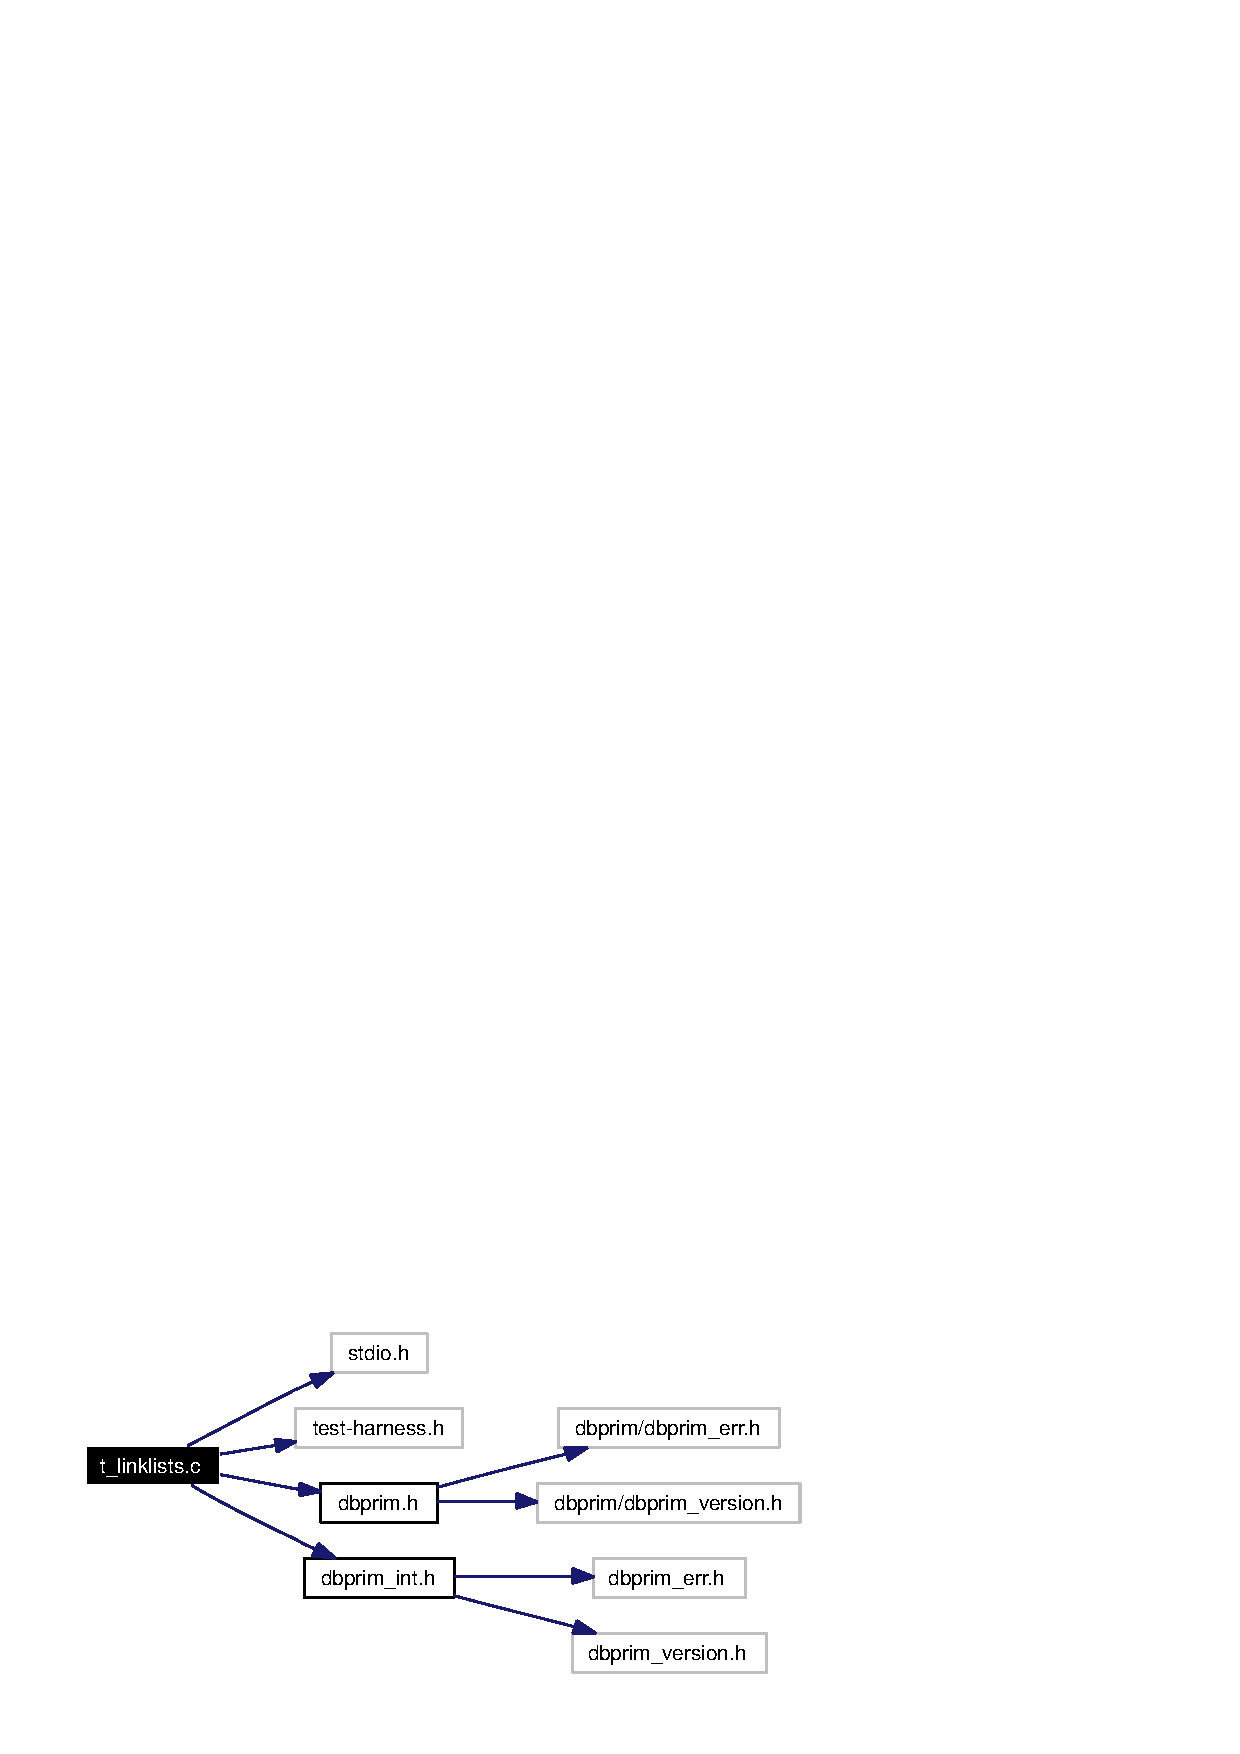
\includegraphics[width=194pt]{t__linklists_8c__incl}
\end{center}
\end{figure}
\subsection*{Data Structures}
\begin{CompactItemize}
\item 
struct \hyperlink{structtdata__s}{tdata\_\-s}
\item 
struct \hyperlink{structtmove__s}{tmove\_\-s}
\item 
struct \hyperlink{structiter__desc}{iter\_\-desc}
\end{CompactItemize}
\subsection*{Defines}
\begin{CompactItemize}
\item 
\#define \hyperlink{t__linklists_8c_a0}{LINK\_\-ELEM\_\-CNT}
\item 
\#define \hyperlink{t__linklists_8c_a1}{LINK\_\-MOVE\_\-CNT}
\item 
\#define \hyperlink{t__linklists_8c_a2}{LINK\_\-REMOVE\_\-CNT}
\item 
\#define \hyperlink{t__linklists_8c_a3}{LINK\_\-ITER\_\-CNT}
\item 
\#define \hyperlink{t__linklists_8c_a4}{LINK\_\-FLUSH\_\-CNT}
\item 
\#define \hyperlink{t__linklists_8c_a5}{Chk\-Order}(name, order, fatal, go)
\end{CompactItemize}
\subsection*{Functions}
\begin{CompactItemize}
\item 
static unsigned long \hyperlink{t__linklists_8c_a15}{t\_\-comp} (\hyperlink{struct__db__key__s}{db\_\-key\_\-t} $\ast$key, void $\ast$comp)
\item 
static unsigned long \hyperlink{t__linklists_8c_a16}{t\_\-iter} (\hyperlink{struct__link__head__s}{link\_\-head\_\-t} $\ast$head, \hyperlink{struct__link__elem__s}{link\_\-elem\_\-t} $\ast$elem, void $\ast$extra)
\item 
int \hyperlink{t__linklists_8c_a17}{main} (int argc, char $\ast$$\ast$argv)
\end{CompactItemize}
\subsection*{Variables}
\begin{CompactItemize}
\item 
\hyperlink{structtdata__s}{tdata\_\-s} \hyperlink{t__linklists_8c_a6}{tdata} \mbox{[}$\,$\mbox{]}
\item 
int \hyperlink{t__linklists_8c_a7}{order\_\-add} \mbox{[}$\,$\mbox{]}
\item 
\hyperlink{structtmove__s}{tmove\_\-s} \hyperlink{t__linklists_8c_a8}{tmove} \mbox{[}$\,$\mbox{]}
\item 
int \hyperlink{t__linklists_8c_a9}{order\_\-move} \mbox{[}$\,$\mbox{]}
\item 
int \hyperlink{t__linklists_8c_a10}{tremove} \mbox{[}$\,$\mbox{]}
\item 
int \hyperlink{t__linklists_8c_a11}{order\_\-remove} \mbox{[}$\,$\mbox{]}
\item 
\hyperlink{structiter__desc}{iter\_\-desc} \hyperlink{t__linklists_8c_a12}{desc\_\-iter} \mbox{[}$\,$\mbox{]}
\item 
\hyperlink{structiter__desc}{iter\_\-desc} \hyperlink{t__linklists_8c_a13}{desc\_\-flush} \mbox{[}$\,$\mbox{]}
\item 
int \hyperlink{t__linklists_8c_a14}{order\_\-flush} \mbox{[}$\,$\mbox{]}\mbox{[}2\mbox{]}
\end{CompactItemize}


\subsection{Define Documentation}
\hypertarget{t__linklists_8c_a5}{
\index{t_linklists.c@{t\_\-linklists.c}!ChkOrder@{ChkOrder}}
\index{ChkOrder@{ChkOrder}!t_linklists.c@{t\_\-linklists.c}}
\subsubsection[ChkOrder]{\setlength{\rightskip}{0pt plus 5cm}\#define Chk\-Order(name, order, fatal, go)}}
\label{t__linklists_8c_a5}




Definition at line 117 of file t\_\-linklists.c.

Referenced by main().\hypertarget{t__linklists_8c_a0}{
\index{t_linklists.c@{t\_\-linklists.c}!LINK_ELEM_CNT@{LINK\_\-ELEM\_\-CNT}}
\index{LINK_ELEM_CNT@{LINK\_\-ELEM\_\-CNT}!t_linklists.c@{t\_\-linklists.c}}
\subsubsection[LINK\_\-ELEM\_\-CNT]{\setlength{\rightskip}{0pt plus 5cm}\#define LINK\_\-ELEM\_\-CNT}}
\label{t__linklists_8c_a0}




Definition at line 44 of file t\_\-linklists.c.

Referenced by main().\hypertarget{t__linklists_8c_a4}{
\index{t_linklists.c@{t\_\-linklists.c}!LINK_FLUSH_CNT@{LINK\_\-FLUSH\_\-CNT}}
\index{LINK_FLUSH_CNT@{LINK\_\-FLUSH\_\-CNT}!t_linklists.c@{t\_\-linklists.c}}
\subsubsection[LINK\_\-FLUSH\_\-CNT]{\setlength{\rightskip}{0pt plus 5cm}\#define LINK\_\-FLUSH\_\-CNT}}
\label{t__linklists_8c_a4}




Definition at line 115 of file t\_\-linklists.c.

Referenced by main().\hypertarget{t__linklists_8c_a3}{
\index{t_linklists.c@{t\_\-linklists.c}!LINK_ITER_CNT@{LINK\_\-ITER\_\-CNT}}
\index{LINK_ITER_CNT@{LINK\_\-ITER\_\-CNT}!t_linklists.c@{t\_\-linklists.c}}
\subsubsection[LINK\_\-ITER\_\-CNT]{\setlength{\rightskip}{0pt plus 5cm}\#define LINK\_\-ITER\_\-CNT}}
\label{t__linklists_8c_a3}




Definition at line 103 of file t\_\-linklists.c.

Referenced by main().\hypertarget{t__linklists_8c_a1}{
\index{t_linklists.c@{t\_\-linklists.c}!LINK_MOVE_CNT@{LINK\_\-MOVE\_\-CNT}}
\index{LINK_MOVE_CNT@{LINK\_\-MOVE\_\-CNT}!t_linklists.c@{t\_\-linklists.c}}
\subsubsection[LINK\_\-MOVE\_\-CNT]{\setlength{\rightskip}{0pt plus 5cm}\#define LINK\_\-MOVE\_\-CNT}}
\label{t__linklists_8c_a1}




Definition at line 59 of file t\_\-linklists.c.

Referenced by main().\hypertarget{t__linklists_8c_a2}{
\index{t_linklists.c@{t\_\-linklists.c}!LINK_REMOVE_CNT@{LINK\_\-REMOVE\_\-CNT}}
\index{LINK_REMOVE_CNT@{LINK\_\-REMOVE\_\-CNT}!t_linklists.c@{t\_\-linklists.c}}
\subsubsection[LINK\_\-REMOVE\_\-CNT]{\setlength{\rightskip}{0pt plus 5cm}\#define LINK\_\-REMOVE\_\-CNT}}
\label{t__linklists_8c_a2}




Definition at line 65 of file t\_\-linklists.c.

Referenced by main().

\subsection{Function Documentation}
\hypertarget{t__linklists_8c_a17}{
\index{t_linklists.c@{t\_\-linklists.c}!main@{main}}
\index{main@{main}!t_linklists.c@{t\_\-linklists.c}}
\subsubsection[main]{\setlength{\rightskip}{0pt plus 5cm}int main (int {\em argc}, char $\ast$$\ast$ {\em argv})}}
\label{t__linklists_8c_a17}




Definition at line 139 of file t\_\-linklists.c.

References Chk\-Order, DB\_\-KEY\_\-INIT, dk\_\-len, iter\_\-desc::elem, iter\_\-desc::err, iter\_\-desc::expected, iter\_\-desc::flags, le\_\-init(), LINK\_\-ELEM\_\-CNT, LINK\_\-FLUSH\_\-CNT, LINK\_\-ITER\_\-CNT, LINK\_\-MOVE\_\-CNT, LINK\_\-REMOVE\_\-CNT, ll\_\-add(), ll\_\-find(), ll\_\-flush(), ll\_\-init(), ll\_\-iter(), ll\_\-move(), ll\_\-remove(), order\_\-add, order\_\-flush, order\_\-move, order\_\-remove, iter\_\-desc::start, t\_\-comp(), t\_\-iter(), tdata, tmove, tremove, and iter\_\-desc::visited.

Here is the call graph for this function:\begin{figure}[H]
\begin{center}
\leavevmode
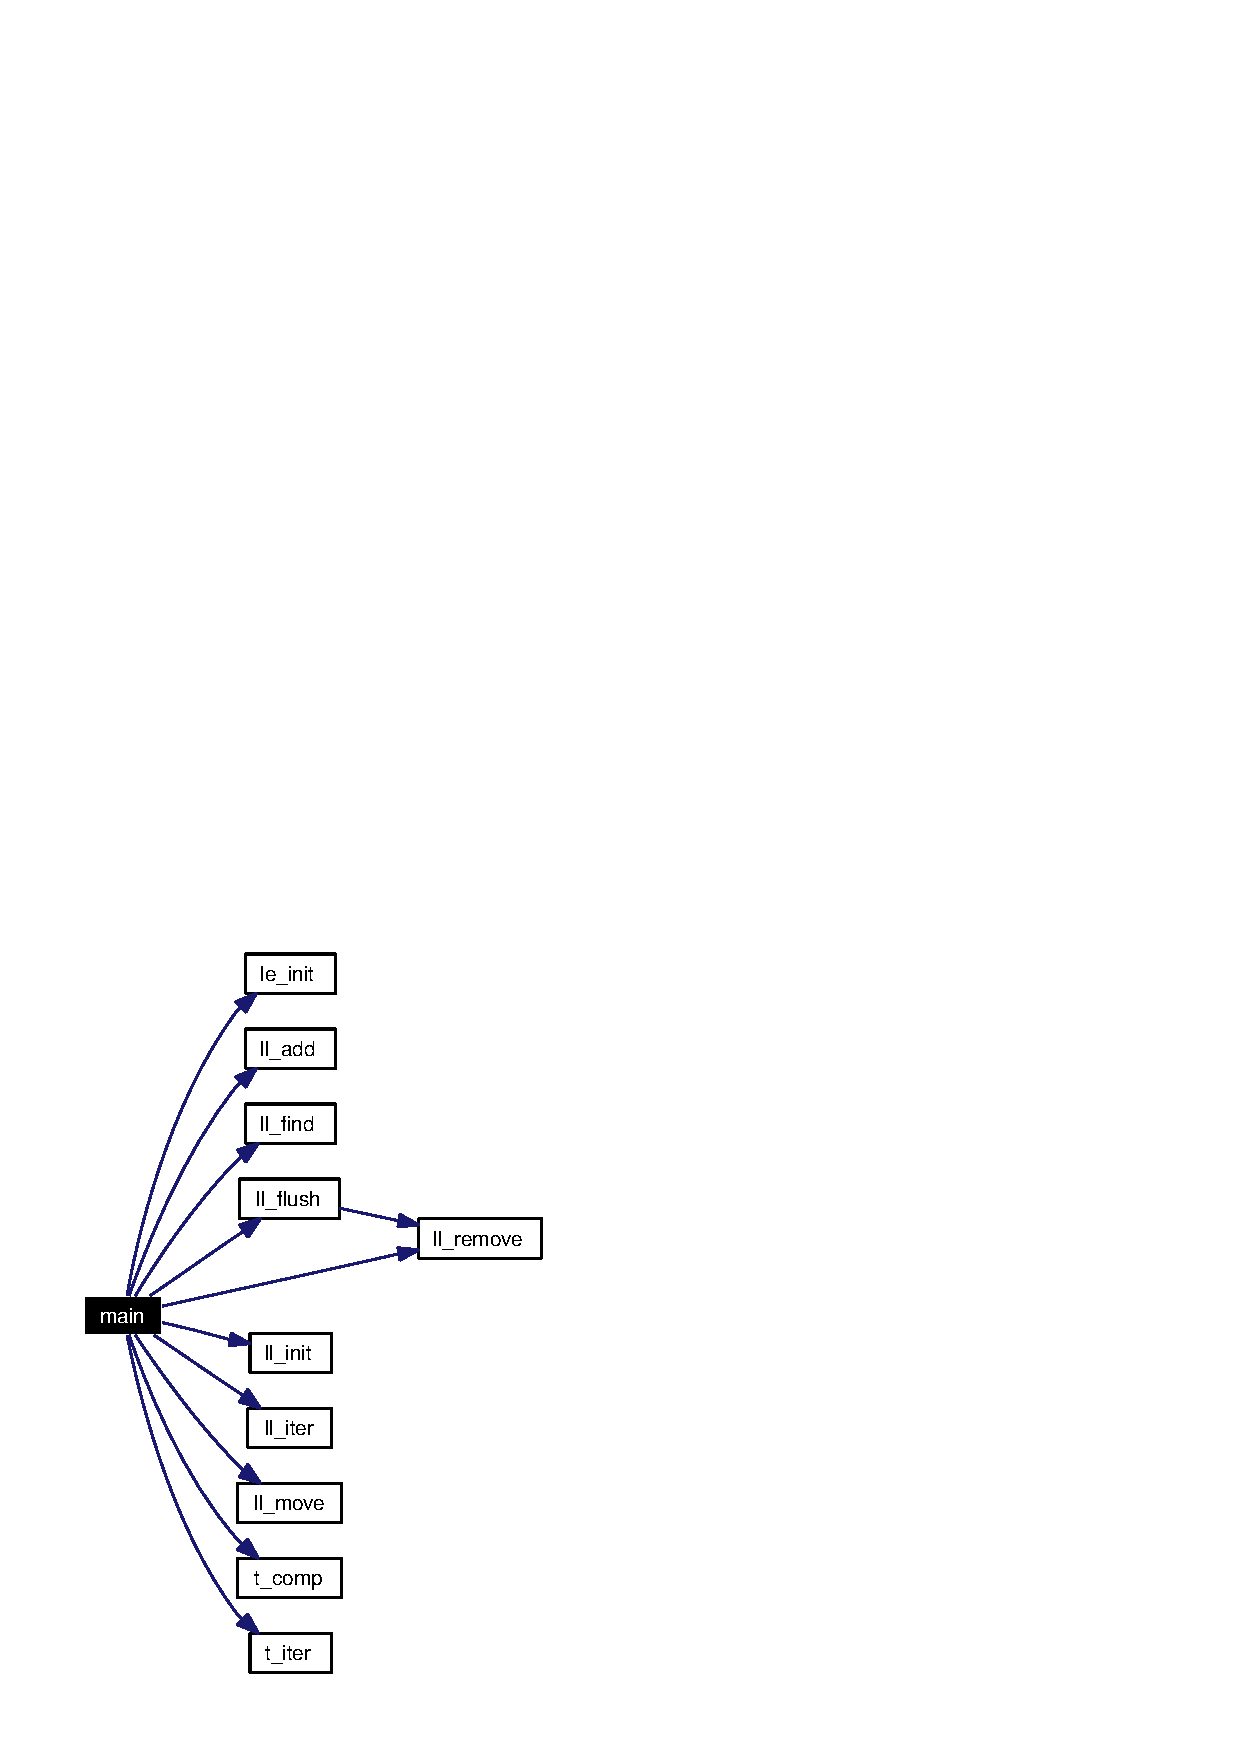
\includegraphics[width=132pt]{t__linklists_8c_a17_cgraph}
\end{center}
\end{figure}
\hypertarget{t__linklists_8c_a15}{
\index{t_linklists.c@{t\_\-linklists.c}!t_comp@{t\_\-comp}}
\index{t_comp@{t\_\-comp}!t_linklists.c@{t\_\-linklists.c}}
\subsubsection[t\_\-comp]{\setlength{\rightskip}{0pt plus 5cm}static unsigned long t\_\-comp (\hyperlink{struct__db__key__s}{db\_\-key\_\-t} $\ast$ {\em key}, void $\ast$ {\em comp})\hspace{0.3cm}{\tt  \mbox{[}static\mbox{]}}}}
\label{t__linklists_8c_a15}




Definition at line 70 of file t\_\-linklists.c.

References dk\_\-len.\hypertarget{t__linklists_8c_a16}{
\index{t_linklists.c@{t\_\-linklists.c}!t_iter@{t\_\-iter}}
\index{t_iter@{t\_\-iter}!t_linklists.c@{t\_\-linklists.c}}
\subsubsection[t\_\-iter]{\setlength{\rightskip}{0pt plus 5cm}static unsigned long t\_\-iter (\hyperlink{struct__link__head__s}{link\_\-head\_\-t} $\ast$ {\em head}, \hyperlink{struct__link__elem__s}{link\_\-elem\_\-t} $\ast$ {\em elem}, void $\ast$ {\em extra})\hspace{0.3cm}{\tt  \mbox{[}static\mbox{]}}}}
\label{t__linklists_8c_a16}




Definition at line 85 of file t\_\-linklists.c.

References iter\_\-desc::elem, iter\_\-desc::err, le\_\-object, and iter\_\-desc::visited.

\subsection{Variable Documentation}
\hypertarget{t__linklists_8c_a13}{
\index{t_linklists.c@{t\_\-linklists.c}!desc_flush@{desc\_\-flush}}
\index{desc_flush@{desc\_\-flush}!t_linklists.c@{t\_\-linklists.c}}
\subsubsection[desc\_\-flush]{\setlength{\rightskip}{0pt plus 5cm}struct \hyperlink{structiter__desc}{iter\_\-desc} \hyperlink{t__linklists_8c_a13}{desc\_\-flush}\mbox{[}$\,$\mbox{]}}}
\label{t__linklists_8c_a13}




Definition at line 105 of file t\_\-linklists.c.\hypertarget{t__linklists_8c_a12}{
\index{t_linklists.c@{t\_\-linklists.c}!desc_iter@{desc\_\-iter}}
\index{desc_iter@{desc\_\-iter}!t_linklists.c@{t\_\-linklists.c}}
\subsubsection[desc\_\-iter]{\setlength{\rightskip}{0pt plus 5cm}struct \hyperlink{structiter__desc}{iter\_\-desc} \hyperlink{t__linklists_8c_a12}{desc\_\-iter}\mbox{[}$\,$\mbox{]}}}
\label{t__linklists_8c_a12}




Definition at line 95 of file t\_\-linklists.c.\hypertarget{t__linklists_8c_a7}{
\index{t_linklists.c@{t\_\-linklists.c}!order_add@{order\_\-add}}
\index{order_add@{order\_\-add}!t_linklists.c@{t\_\-linklists.c}}
\subsubsection[order\_\-add]{\setlength{\rightskip}{0pt plus 5cm}int \hyperlink{t__linklists_8c_a7}{order\_\-add}\mbox{[}$\,$\mbox{]}}}
\label{t__linklists_8c_a7}




Definition at line 46 of file t\_\-linklists.c.

Referenced by main().\hypertarget{t__linklists_8c_a14}{
\index{t_linklists.c@{t\_\-linklists.c}!order_flush@{order\_\-flush}}
\index{order_flush@{order\_\-flush}!t_linklists.c@{t\_\-linklists.c}}
\subsubsection[order\_\-flush]{\setlength{\rightskip}{0pt plus 5cm}int \hyperlink{t__linklists_8c_a14}{order\_\-flush}\mbox{[}$\,$\mbox{]}\mbox{[}2\mbox{]}}}
\label{t__linklists_8c_a14}




Definition at line 110 of file t\_\-linklists.c.

Referenced by main().\hypertarget{t__linklists_8c_a9}{
\index{t_linklists.c@{t\_\-linklists.c}!order_move@{order\_\-move}}
\index{order_move@{order\_\-move}!t_linklists.c@{t\_\-linklists.c}}
\subsubsection[order\_\-move]{\setlength{\rightskip}{0pt plus 5cm}int \hyperlink{t__linklists_8c_a9}{order\_\-move}\mbox{[}$\,$\mbox{]}}}
\label{t__linklists_8c_a9}




Definition at line 61 of file t\_\-linklists.c.

Referenced by main().\hypertarget{t__linklists_8c_a11}{
\index{t_linklists.c@{t\_\-linklists.c}!order_remove@{order\_\-remove}}
\index{order_remove@{order\_\-remove}!t_linklists.c@{t\_\-linklists.c}}
\subsubsection[order\_\-remove]{\setlength{\rightskip}{0pt plus 5cm}int \hyperlink{t__linklists_8c_a11}{order\_\-remove}\mbox{[}$\,$\mbox{]}}}
\label{t__linklists_8c_a11}




Definition at line 67 of file t\_\-linklists.c.

Referenced by main().\hypertarget{t__linklists_8c_a6}{
\index{t_linklists.c@{t\_\-linklists.c}!tdata@{tdata}}
\index{tdata@{tdata}!t_linklists.c@{t\_\-linklists.c}}
\subsubsection[tdata]{\setlength{\rightskip}{0pt plus 5cm}struct \hyperlink{structtdata__s}{tdata\_\-s}  \hyperlink{t__linklists_8c_a6}{tdata}\mbox{[}$\,$\mbox{]}}}
\label{t__linklists_8c_a6}




Referenced by main().\hypertarget{t__linklists_8c_a8}{
\index{t_linklists.c@{t\_\-linklists.c}!tmove@{tmove}}
\index{tmove@{tmove}!t_linklists.c@{t\_\-linklists.c}}
\subsubsection[tmove]{\setlength{\rightskip}{0pt plus 5cm}struct \hyperlink{structtmove__s}{tmove\_\-s}  \hyperlink{t__linklists_8c_a8}{tmove}\mbox{[}$\,$\mbox{]}}}
\label{t__linklists_8c_a8}




Referenced by main().\hypertarget{t__linklists_8c_a10}{
\index{t_linklists.c@{t\_\-linklists.c}!tremove@{tremove}}
\index{tremove@{tremove}!t_linklists.c@{t\_\-linklists.c}}
\subsubsection[tremove]{\setlength{\rightskip}{0pt plus 5cm}int \hyperlink{t__linklists_8c_a10}{tremove}\mbox{[}$\,$\mbox{]}}}
\label{t__linklists_8c_a10}




Definition at line 63 of file t\_\-linklists.c.

Referenced by main().
\hypertarget{t__redblack_8c}{
\section{t\_\-redblack.c File Reference}
\label{t__redblack_8c}\index{t_redblack.c@{t\_\-redblack.c}}
}


{\tt \#include $<$assert.h$>$}\par
{\tt \#include $<$stdio.h$>$}\par
{\tt \#include $<$stdlib.h$>$}\par
{\tt \#include $<$string.h$>$}\par
{\tt \#include $<$time.h$>$}\par
{\tt \#include \char`\"{}test-harness.h\char`\"{}}\par
{\tt \#include \char`\"{}dbprim.h\char`\"{}}\par
{\tt \#include \char`\"{}dbprim\_\-int.h\char`\"{}}\par


Include dependency graph for t\_\-redblack.c:\begin{figure}[H]
\begin{center}
\leavevmode
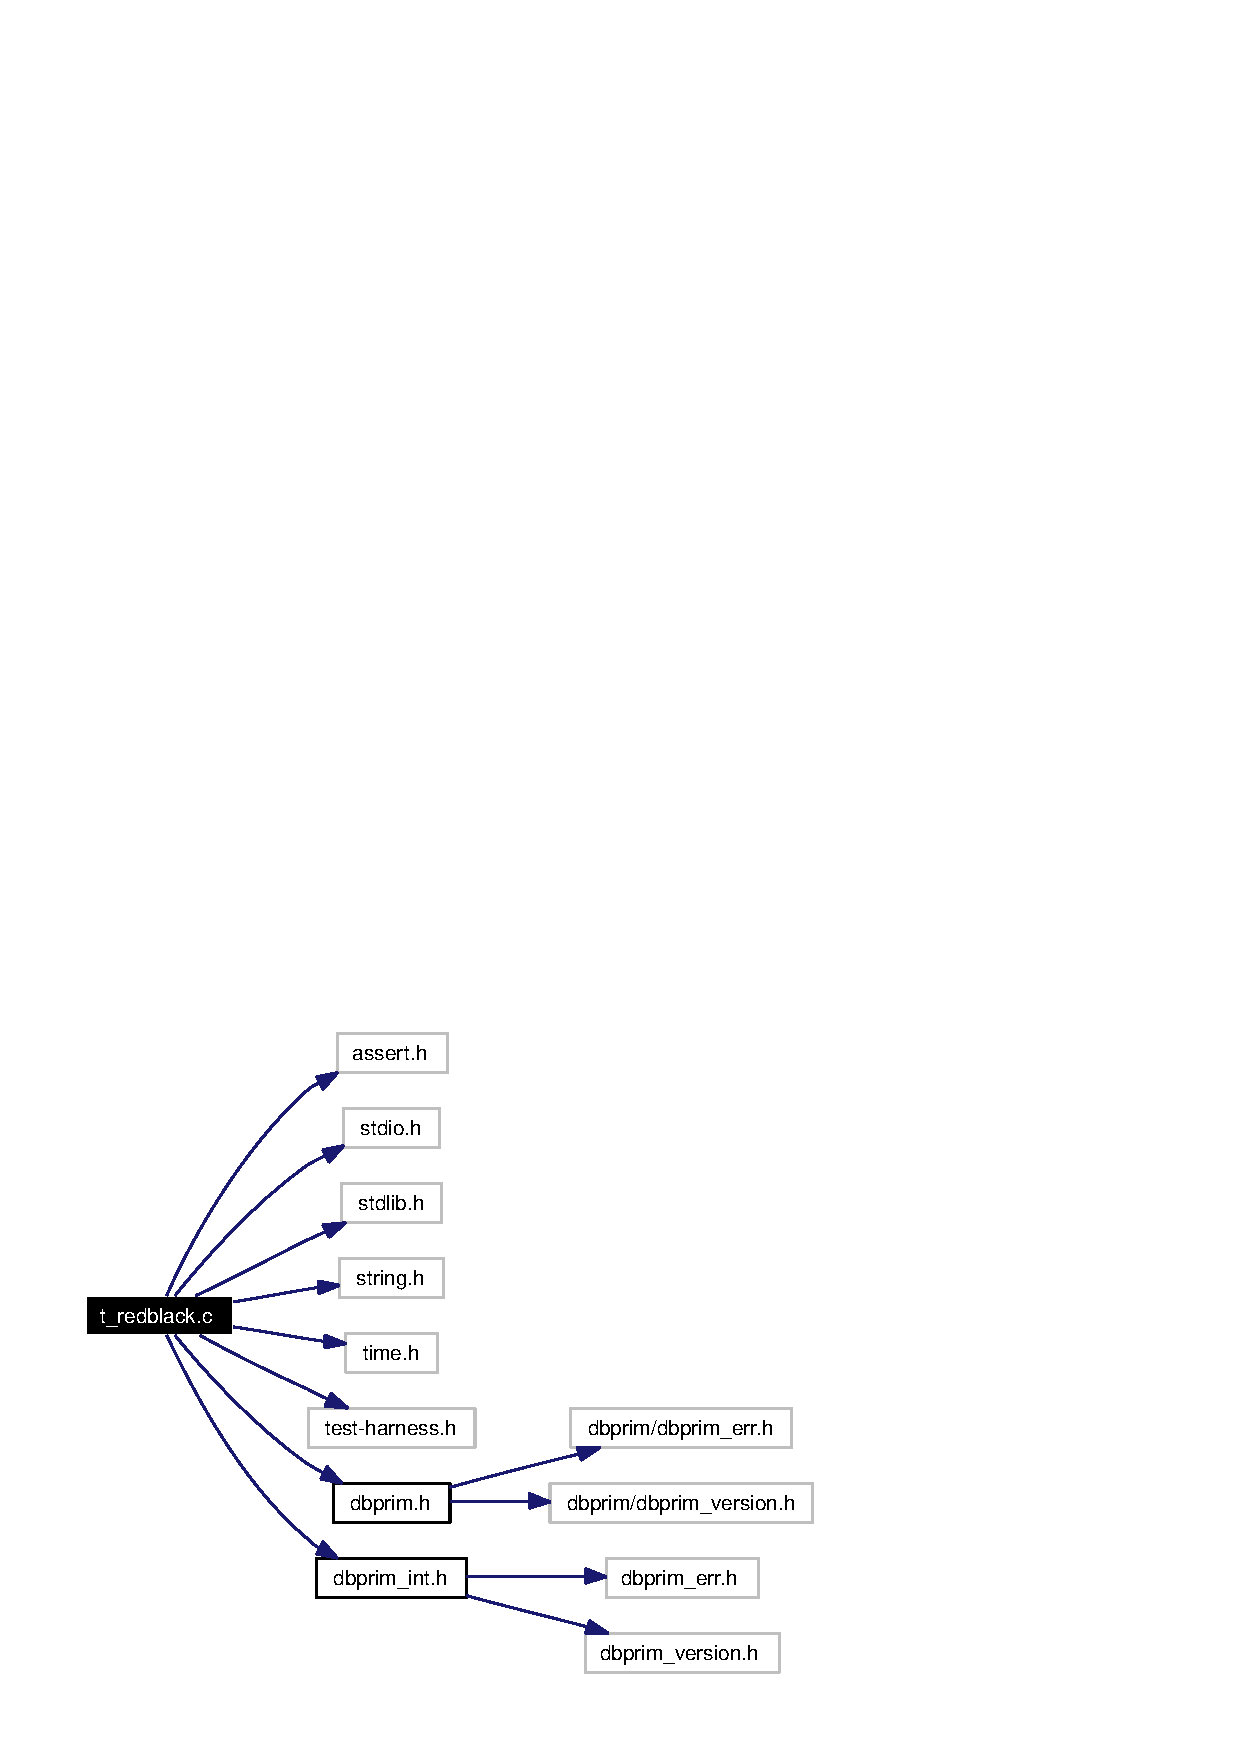
\includegraphics[width=197pt]{t__redblack_8c__incl}
\end{center}
\end{figure}
\subsection*{Data Structures}
\begin{CompactItemize}
\item 
struct \hyperlink{structflush__test}{flush\_\-test}
\item 
struct \hyperlink{structiter__test}{iter\_\-test}
\end{CompactItemize}
\subsection*{Defines}
\begin{CompactItemize}
\item 
\#define \hyperlink{t__redblack_8c_a0}{RBT\_\-ELEM\_\-CNT}
\item 
\#define \hyperlink{t__redblack_8c_a1}{RBT\_\-ELEM\_\-MASK}
\item 
\#define \hyperlink{t__redblack_8c_a2}{selnode}(n, rev)
\item 
\#define \hyperlink{t__redblack_8c_a3}{n\_\-debargs}(node)
\item 
\#define \hyperlink{t__redblack_8c_a4}{STOP\_\-RETURN}
\item 
\#define \hyperlink{t__redblack_8c_a5}{VISIT\_\-RETURN}
\item 
\#define \hyperlink{t__redblack_8c_a6}{ITER\_\-TRIALS}
\end{CompactItemize}
\subsection*{Functions}
\begin{CompactItemize}
\item 
static void \hyperlink{t__redblack_8c_a7}{\_\-make\_\-pre} (\hyperlink{struct__rb__node__s}{rb\_\-node\_\-t} $\ast$node, int $\ast$order, int $\ast$idx, int reverse, unsigned long $\ast$visited)
\item 
static void \hyperlink{t__redblack_8c_a8}{\_\-make\_\-in} (\hyperlink{struct__rb__node__s}{rb\_\-node\_\-t} $\ast$node, int $\ast$order, int $\ast$idx, int reverse, unsigned long $\ast$visited)
\item 
static void \hyperlink{t__redblack_8c_a9}{\_\-make\_\-post} (\hyperlink{struct__rb__node__s}{rb\_\-node\_\-t} $\ast$node, int $\ast$order, int $\ast$idx, int reverse, unsigned long $\ast$visited)
\item 
static void \hyperlink{t__redblack_8c_a10}{make\_\-order} (\hyperlink{struct__rb__tree__s}{rb\_\-tree\_\-t} $\ast$tree, int $\ast$order, unsigned long flags, unsigned long $\ast$visited)
\item 
static int \hyperlink{t__redblack_8c_a11}{comp\_\-order} (int $\ast$o1, int $\ast$o2)
\item 
static int \hyperlink{t__redblack_8c_a12}{treecheck} (\hyperlink{struct__rb__node__s}{rb\_\-node\_\-t} $\ast$node, \hyperlink{struct__rb__node__s}{rb\_\-node\_\-t} $\ast$parent, int bh, int $\ast$tbhp)
\item 
static long \hyperlink{t__redblack_8c_a13}{t\_\-comp} (\hyperlink{struct__rb__tree__s}{rb\_\-tree\_\-t} $\ast$tree, \hyperlink{struct__db__key__s}{db\_\-key\_\-t} $\ast$key1, \hyperlink{struct__db__key__s}{db\_\-key\_\-t} $\ast$key2)
\item 
static unsigned long \hyperlink{t__redblack_8c_a14}{t\_\-flush} (\hyperlink{struct__rb__tree__s}{rb\_\-tree\_\-t} $\ast$tree, \hyperlink{struct__rb__node__s}{rb\_\-node\_\-t} $\ast$node, struct \hyperlink{structflush__test}{flush\_\-test} $\ast$ft)
\item 
static unsigned long \hyperlink{t__redblack_8c_a15}{t\_\-iter} (\hyperlink{struct__rb__tree__s}{rb\_\-tree\_\-t} $\ast$tree, \hyperlink{struct__rb__node__s}{rb\_\-node\_\-t} $\ast$node, struct \hyperlink{structiter__test}{iter\_\-test} $\ast$it)
\item 
int \hyperlink{t__redblack_8c_a16}{main} (int argc, char $\ast$$\ast$argv)
\end{CompactItemize}


\subsection{Define Documentation}
\hypertarget{t__redblack_8c_a6}{
\index{t_redblack.c@{t\_\-redblack.c}!ITER_TRIALS@{ITER\_\-TRIALS}}
\index{ITER_TRIALS@{ITER\_\-TRIALS}!t_redblack.c@{t\_\-redblack.c}}
\subsubsection[ITER\_\-TRIALS]{\setlength{\rightskip}{0pt plus 5cm}\#define ITER\_\-TRIALS}}
\label{t__redblack_8c_a6}




Definition at line 268 of file t\_\-redblack.c.

Referenced by main().\hypertarget{t__redblack_8c_a3}{
\index{t_redblack.c@{t\_\-redblack.c}!n_debargs@{n\_\-debargs}}
\index{n_debargs@{n\_\-debargs}!t_redblack.c@{t\_\-redblack.c}}
\subsubsection[n\_\-debargs]{\setlength{\rightskip}{0pt plus 5cm}\#define n\_\-debargs(node)}}
\label{t__redblack_8c_a3}




Definition at line 134 of file t\_\-redblack.c.

Referenced by treecheck().\hypertarget{t__redblack_8c_a0}{
\index{t_redblack.c@{t\_\-redblack.c}!RBT_ELEM_CNT@{RBT\_\-ELEM\_\-CNT}}
\index{RBT_ELEM_CNT@{RBT\_\-ELEM\_\-CNT}!t_redblack.c@{t\_\-redblack.c}}
\subsubsection[RBT\_\-ELEM\_\-CNT]{\setlength{\rightskip}{0pt plus 5cm}\#define RBT\_\-ELEM\_\-CNT}}
\label{t__redblack_8c_a0}




Definition at line 36 of file t\_\-redblack.c.

Referenced by comp\_\-order(), and main().\hypertarget{t__redblack_8c_a1}{
\index{t_redblack.c@{t\_\-redblack.c}!RBT_ELEM_MASK@{RBT\_\-ELEM\_\-MASK}}
\index{RBT_ELEM_MASK@{RBT\_\-ELEM\_\-MASK}!t_redblack.c@{t\_\-redblack.c}}
\subsubsection[RBT\_\-ELEM\_\-MASK]{\setlength{\rightskip}{0pt plus 5cm}\#define RBT\_\-ELEM\_\-MASK}}
\label{t__redblack_8c_a1}




Definition at line 42 of file t\_\-redblack.c.

Referenced by main().\hypertarget{t__redblack_8c_a2}{
\index{t_redblack.c@{t\_\-redblack.c}!selnode@{selnode}}
\index{selnode@{selnode}!t_redblack.c@{t\_\-redblack.c}}
\subsubsection[selnode]{\setlength{\rightskip}{0pt plus 5cm}\#define selnode(n, rev)}}
\label{t__redblack_8c_a2}




Referenced by \_\-make\_\-in().\hypertarget{t__redblack_8c_a4}{
\index{t_redblack.c@{t\_\-redblack.c}!STOP_RETURN@{STOP\_\-RETURN}}
\index{STOP_RETURN@{STOP\_\-RETURN}!t_redblack.c@{t\_\-redblack.c}}
\subsubsection[STOP\_\-RETURN]{\setlength{\rightskip}{0pt plus 5cm}\#define STOP\_\-RETURN}}
\label{t__redblack_8c_a4}




Definition at line 239 of file t\_\-redblack.c.

Referenced by main(), t\_\-flush(), and t\_\-iter().\hypertarget{t__redblack_8c_a5}{
\index{t_redblack.c@{t\_\-redblack.c}!VISIT_RETURN@{VISIT\_\-RETURN}}
\index{VISIT_RETURN@{VISIT\_\-RETURN}!t_redblack.c@{t\_\-redblack.c}}
\subsubsection[VISIT\_\-RETURN]{\setlength{\rightskip}{0pt plus 5cm}\#define VISIT\_\-RETURN}}
\label{t__redblack_8c_a5}




Definition at line 240 of file t\_\-redblack.c.

Referenced by main(), t\_\-flush(), and t\_\-iter().

\subsection{Function Documentation}
\hypertarget{t__redblack_8c_a8}{
\index{t_redblack.c@{t\_\-redblack.c}!_make_in@{\_\-make\_\-in}}
\index{_make_in@{\_\-make\_\-in}!t_redblack.c@{t\_\-redblack.c}}
\subsubsection[\_\-make\_\-in]{\setlength{\rightskip}{0pt plus 5cm}static void \_\-make\_\-in (\hyperlink{struct__rb__node__s}{rb\_\-node\_\-t} $\ast$ {\em node}, int $\ast$ {\em order}, int $\ast$ {\em idx}, int {\em reverse}, unsigned long $\ast$ {\em visited})\hspace{0.3cm}{\tt  \mbox{[}static\mbox{]}}}}
\label{t__redblack_8c_a8}




Definition at line 62 of file t\_\-redblack.c.

References rn\_\-value, and selnode.

Referenced by make\_\-order().\hypertarget{t__redblack_8c_a9}{
\index{t_redblack.c@{t\_\-redblack.c}!_make_post@{\_\-make\_\-post}}
\index{_make_post@{\_\-make\_\-post}!t_redblack.c@{t\_\-redblack.c}}
\subsubsection[\_\-make\_\-post]{\setlength{\rightskip}{0pt plus 5cm}static void \_\-make\_\-post (\hyperlink{struct__rb__node__s}{rb\_\-node\_\-t} $\ast$ {\em node}, int $\ast$ {\em order}, int $\ast$ {\em idx}, int {\em reverse}, unsigned long $\ast$ {\em visited})\hspace{0.3cm}{\tt  \mbox{[}static\mbox{]}}}}
\label{t__redblack_8c_a9}




Definition at line 77 of file t\_\-redblack.c.

References rn\_\-left, rn\_\-right, and rn\_\-value.

Referenced by make\_\-order().\hypertarget{t__redblack_8c_a7}{
\index{t_redblack.c@{t\_\-redblack.c}!_make_pre@{\_\-make\_\-pre}}
\index{_make_pre@{\_\-make\_\-pre}!t_redblack.c@{t\_\-redblack.c}}
\subsubsection[\_\-make\_\-pre]{\setlength{\rightskip}{0pt plus 5cm}static void \_\-make\_\-pre (\hyperlink{struct__rb__node__s}{rb\_\-node\_\-t} $\ast$ {\em node}, int $\ast$ {\em order}, int $\ast$ {\em idx}, int {\em reverse}, unsigned long $\ast$ {\em visited})\hspace{0.3cm}{\tt  \mbox{[}static\mbox{]}}}}
\label{t__redblack_8c_a7}




Definition at line 46 of file t\_\-redblack.c.

References rn\_\-left, rn\_\-right, and rn\_\-value.

Referenced by make\_\-order().\hypertarget{t__redblack_8c_a11}{
\index{t_redblack.c@{t\_\-redblack.c}!comp_order@{comp\_\-order}}
\index{comp_order@{comp\_\-order}!t_redblack.c@{t\_\-redblack.c}}
\subsubsection[comp\_\-order]{\setlength{\rightskip}{0pt plus 5cm}static int comp\_\-order (int $\ast$ {\em o1}, int $\ast$ {\em o2})\hspace{0.3cm}{\tt  \mbox{[}static\mbox{]}}}}
\label{t__redblack_8c_a11}




Definition at line 116 of file t\_\-redblack.c.

References RBT\_\-ELEM\_\-CNT.

Referenced by main().\hypertarget{t__redblack_8c_a16}{
\index{t_redblack.c@{t\_\-redblack.c}!main@{main}}
\index{main@{main}!t_redblack.c@{t\_\-redblack.c}}
\subsubsection[main]{\setlength{\rightskip}{0pt plus 5cm}int main (int {\em argc}, char $\ast$$\ast$ {\em argv})}}
\label{t__redblack_8c_a16}




Definition at line 293 of file t\_\-redblack.c.

References comp\_\-order(), DB\_\-KEY\_\-INIT, dk\_\-len, iter\_\-test::idx, ITER\_\-TRIALS, iter\_\-test::last\_\-node, make\_\-order(), iter\_\-test::order, RBT\_\-ELEM\_\-CNT, RBT\_\-ELEM\_\-MASK, RBT\_\-ORDER\_\-MASK, rn\_\-init(), rn\_\-key, rt\_\-add(), rt\_\-count, rt\_\-find(), rt\_\-flush(), rt\_\-init(), rt\_\-iter(), rt\_\-next(), rt\_\-remove(), rt\_\-root, iter\_\-test::stop\_\-node, flush\_\-test::stop\_\-node, STOP\_\-RETURN, t\_\-comp(), t\_\-flush(), t\_\-iter(), treecheck(), VISIT\_\-RETURN, iter\_\-test::visited, and flush\_\-test::visited.

Here is the call graph for this function:\begin{figure}[H]
\begin{center}
\leavevmode
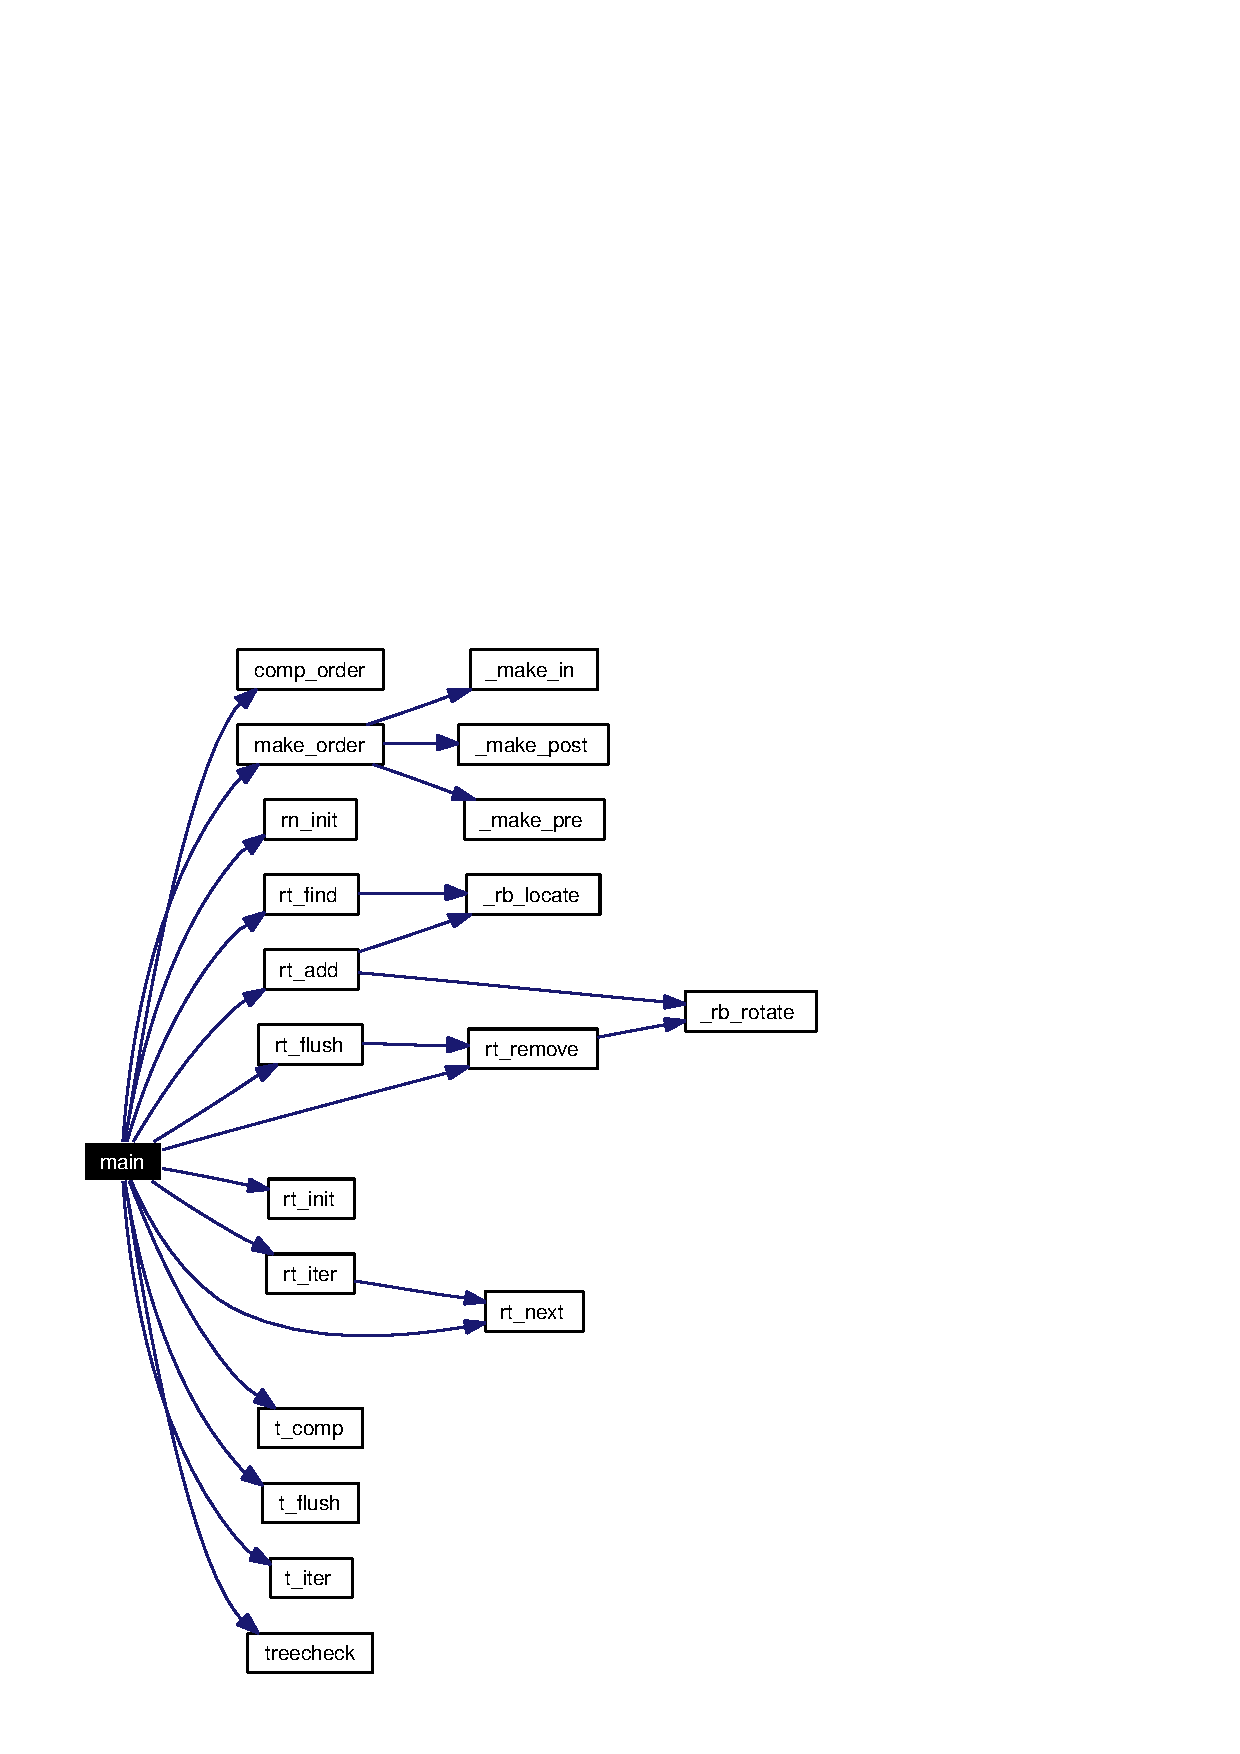
\includegraphics[width=198pt]{t__redblack_8c_a16_cgraph}
\end{center}
\end{figure}
\hypertarget{t__redblack_8c_a10}{
\index{t_redblack.c@{t\_\-redblack.c}!make_order@{make\_\-order}}
\index{make_order@{make\_\-order}!t_redblack.c@{t\_\-redblack.c}}
\subsubsection[make\_\-order]{\setlength{\rightskip}{0pt plus 5cm}static void make\_\-order (\hyperlink{struct__rb__tree__s}{rb\_\-tree\_\-t} $\ast$ {\em tree}, int $\ast$ {\em order}, unsigned long {\em flags}, unsigned long $\ast$ {\em visited})\hspace{0.3cm}{\tt  \mbox{[}static\mbox{]}}}}
\label{t__redblack_8c_a10}




Definition at line 93 of file t\_\-redblack.c.

References \_\-make\_\-in(), \_\-make\_\-post(), \_\-make\_\-pre(), DB\_\-FLAG\_\-REVERSE, RBT\_\-ORDER\_\-IN, RBT\_\-ORDER\_\-POST, RBT\_\-ORDER\_\-PRE, and rt\_\-root.

Referenced by main().

Here is the call graph for this function:\begin{figure}[H]
\begin{center}
\leavevmode
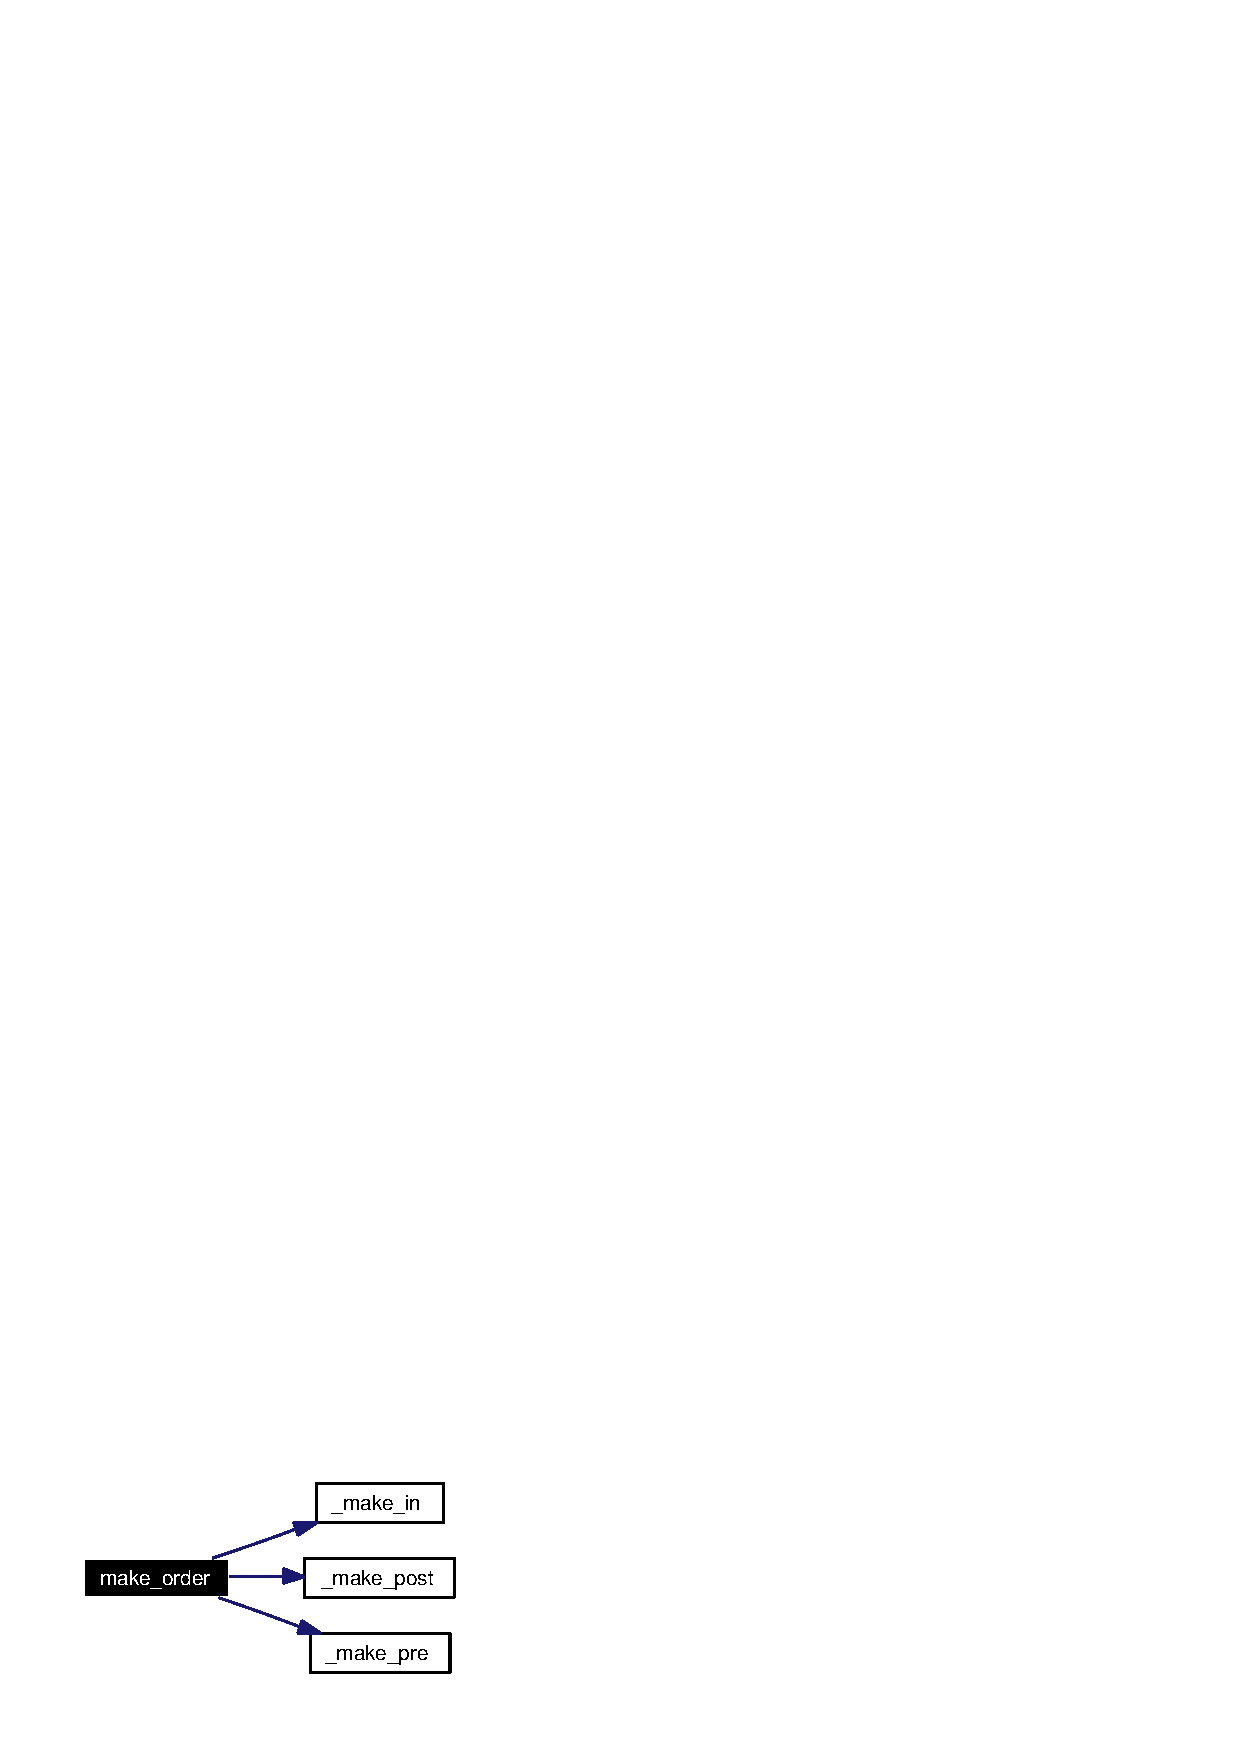
\includegraphics[width=111pt]{t__redblack_8c_a10_cgraph}
\end{center}
\end{figure}
\hypertarget{t__redblack_8c_a13}{
\index{t_redblack.c@{t\_\-redblack.c}!t_comp@{t\_\-comp}}
\index{t_comp@{t\_\-comp}!t_redblack.c@{t\_\-redblack.c}}
\subsubsection[t\_\-comp]{\setlength{\rightskip}{0pt plus 5cm}static long t\_\-comp (\hyperlink{struct__rb__tree__s}{rb\_\-tree\_\-t} $\ast$ {\em tree}, \hyperlink{struct__db__key__s}{db\_\-key\_\-t} $\ast$ {\em key1}, \hyperlink{struct__db__key__s}{db\_\-key\_\-t} $\ast$ {\em key2})\hspace{0.3cm}{\tt  \mbox{[}static\mbox{]}}}}
\label{t__redblack_8c_a13}




Definition at line 228 of file t\_\-redblack.c.

References dk\_\-len.\hypertarget{t__redblack_8c_a14}{
\index{t_redblack.c@{t\_\-redblack.c}!t_flush@{t\_\-flush}}
\index{t_flush@{t\_\-flush}!t_redblack.c@{t\_\-redblack.c}}
\subsubsection[t\_\-flush]{\setlength{\rightskip}{0pt plus 5cm}static unsigned long t\_\-flush (\hyperlink{struct__rb__tree__s}{rb\_\-tree\_\-t} $\ast$ {\em tree}, \hyperlink{struct__rb__node__s}{rb\_\-node\_\-t} $\ast$ {\em node}, struct \hyperlink{structflush__test}{flush\_\-test} $\ast$ {\em ft})\hspace{0.3cm}{\tt  \mbox{[}static\mbox{]}}}}
\label{t__redblack_8c_a14}




Definition at line 244 of file t\_\-redblack.c.

References dk\_\-len, rn\_\-key, flush\_\-test::stop\_\-node, STOP\_\-RETURN, VISIT\_\-RETURN, and flush\_\-test::visited.

Referenced by main().\hypertarget{t__redblack_8c_a15}{
\index{t_redblack.c@{t\_\-redblack.c}!t_iter@{t\_\-iter}}
\index{t_iter@{t\_\-iter}!t_redblack.c@{t\_\-redblack.c}}
\subsubsection[t\_\-iter]{\setlength{\rightskip}{0pt plus 5cm}static unsigned long t\_\-iter (\hyperlink{struct__rb__tree__s}{rb\_\-tree\_\-t} $\ast$ {\em tree}, \hyperlink{struct__rb__node__s}{rb\_\-node\_\-t} $\ast$ {\em node}, struct \hyperlink{structiter__test}{iter\_\-test} $\ast$ {\em it})\hspace{0.3cm}{\tt  \mbox{[}static\mbox{]}}}}
\label{t__redblack_8c_a15}




Definition at line 272 of file t\_\-redblack.c.

References dk\_\-len, iter\_\-test::idx, iter\_\-test::last\_\-node, iter\_\-test::order, rn\_\-key, iter\_\-test::stop\_\-node, STOP\_\-RETURN, VISIT\_\-RETURN, and iter\_\-test::visited.\hypertarget{t__redblack_8c_a12}{
\index{t_redblack.c@{t\_\-redblack.c}!treecheck@{treecheck}}
\index{treecheck@{treecheck}!t_redblack.c@{t\_\-redblack.c}}
\subsubsection[treecheck]{\setlength{\rightskip}{0pt plus 5cm}static int treecheck (\hyperlink{struct__rb__node__s}{rb\_\-node\_\-t} $\ast$ {\em node}, \hyperlink{struct__rb__node__s}{rb\_\-node\_\-t} $\ast$ {\em parent}, int {\em bh}, int $\ast$ {\em tbhp})\hspace{0.3cm}{\tt  \mbox{[}static\mbox{]}}}}
\label{t__redblack_8c_a12}




Definition at line 140 of file t\_\-redblack.c.

References dk\_\-len, n\_\-debargs, rn\_\-isblack, rn\_\-isred, rn\_\-key, \_\-rb\_\-node\_\-s::rn\_\-left, \_\-rb\_\-node\_\-s::rn\_\-parent, and \_\-rb\_\-node\_\-s::rn\_\-right.

Referenced by main().
\hypertarget{t__smat_8c}{
\section{t\_\-smat.c File Reference}
\label{t__smat_8c}\index{t_smat.c@{t\_\-smat.c}}
}


{\tt \#include $<$stdio.h$>$}\par
{\tt \#include $<$stdlib.h$>$}\par
{\tt \#include $<$time.h$>$}\par
{\tt \#include \char`\"{}test-harness.h\char`\"{}}\par
{\tt \#include \char`\"{}dbprim.h\char`\"{}}\par
{\tt \#include \char`\"{}dbprim\_\-int.h\char`\"{}}\par


Include dependency graph for t\_\-smat.c:\begin{figure}[H]
\begin{center}
\leavevmode
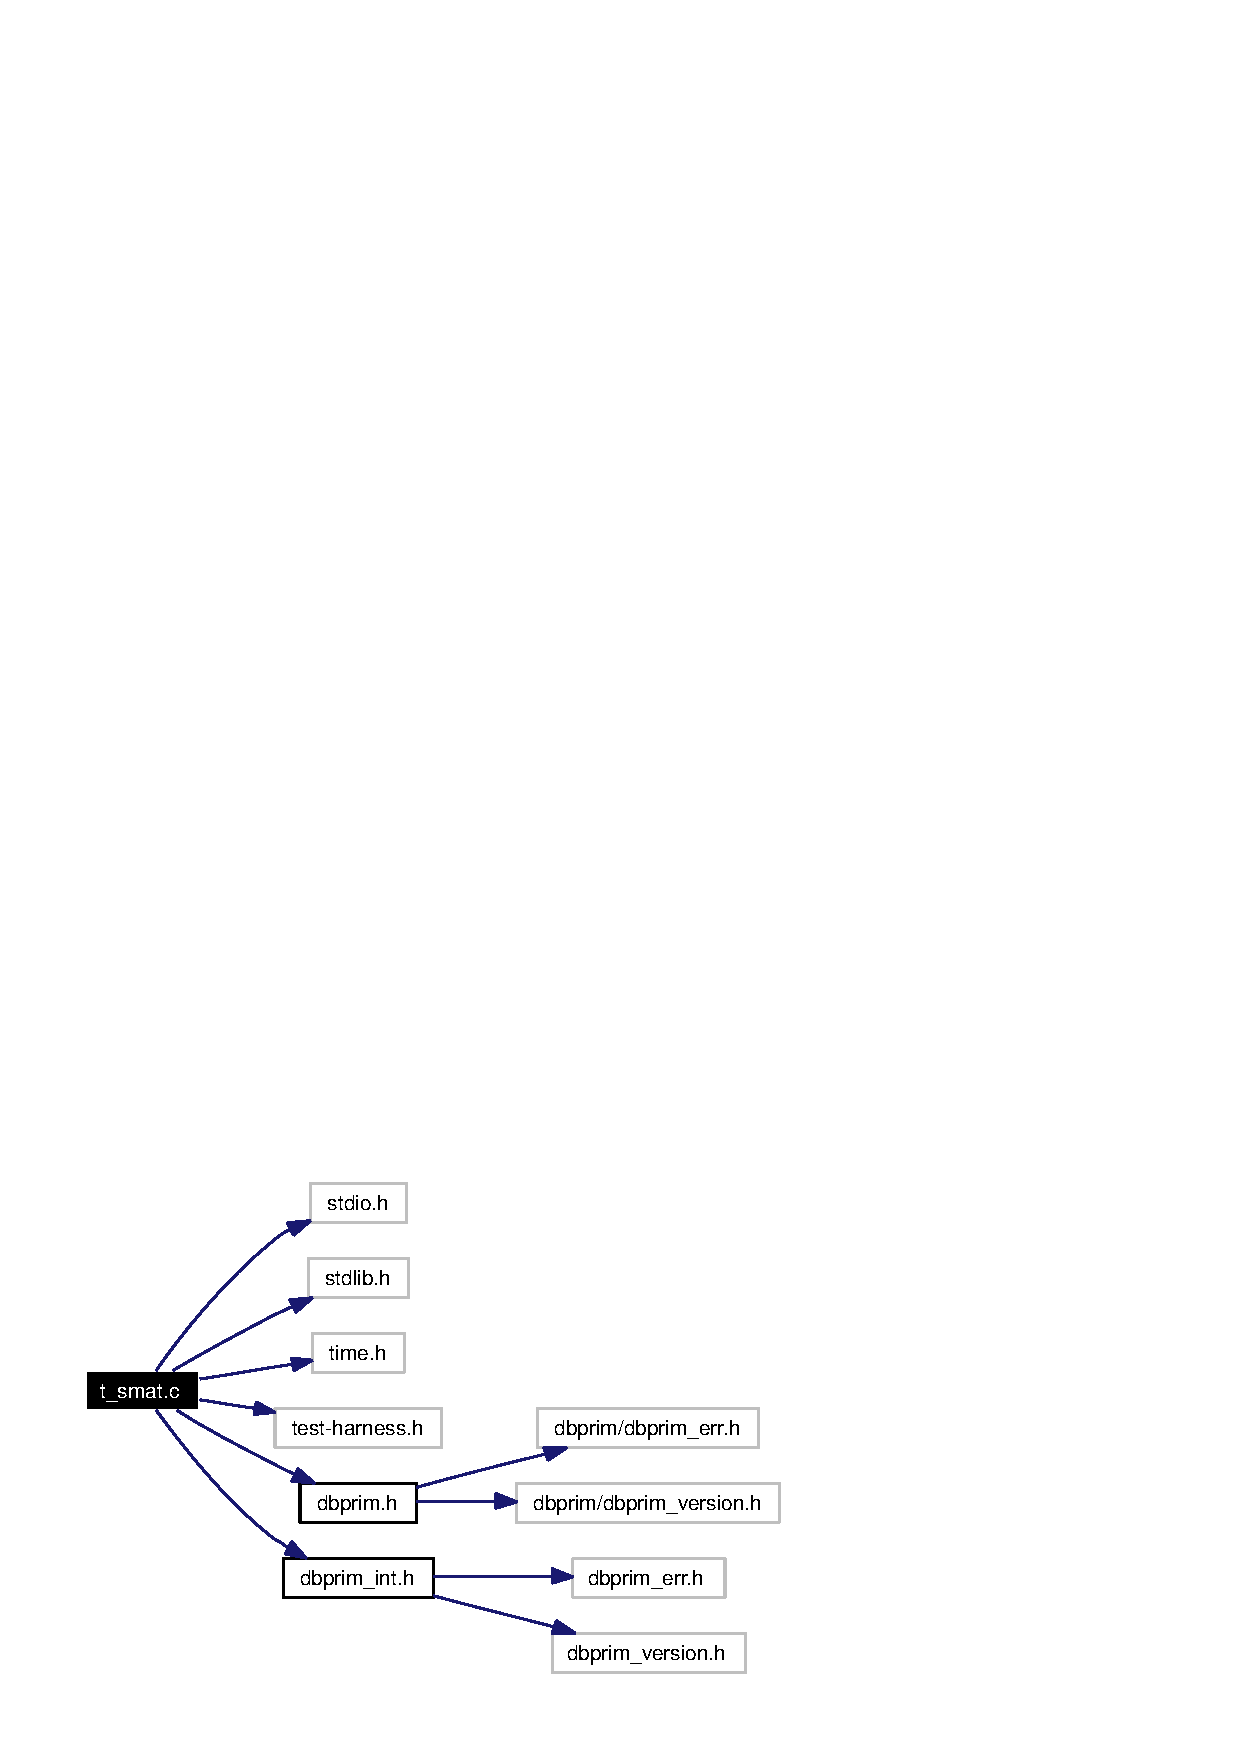
\includegraphics[width=189pt]{t__smat_8c__incl}
\end{center}
\end{figure}
\subsection*{Data Structures}
\begin{CompactItemize}
\item 
struct \hyperlink{structassoc__s}{assoc\_\-s}
\end{CompactItemize}
\subsection*{Defines}
\begin{CompactItemize}
\item 
\#define \hyperlink{t__smat_8c_a0}{SMAT\_\-HEAD\_\-CNT}
\item 
\#define \hyperlink{t__smat_8c_a1}{SMAT\_\-HEAD\_\-MASK}
\item 
\#define \hyperlink{t__smat_8c_a2}{SMAT\_\-ASSOC\_\-CNT}
\item 
\#define \hyperlink{t__smat_8c_a3}{set\_\-assoc}(ass, row, column)
\item 
\#define \hyperlink{t__smat_8c_a4}{clr\_\-assoc}(ass, row, column)
\item 
\#define \hyperlink{t__smat_8c_a5}{chk\_\-assoc}(ass, row, column)
\end{CompactItemize}
\subsection*{Functions}
\begin{CompactItemize}
\item 
static void \hyperlink{t__smat_8c_a9}{set\_\-ones} (struct \hyperlink{structassoc__s}{assoc\_\-s} $\ast$assoc)
\item 
static void \hyperlink{t__smat_8c_a10}{set\_\-zeros} (struct \hyperlink{structassoc__s}{assoc\_\-s} $\ast$assoc)
\item 
static int \hyperlink{t__smat_8c_a11}{check\_\-zeros} (struct \hyperlink{structassoc__s}{assoc\_\-s} $\ast$assoc)
\item 
int \hyperlink{t__smat_8c_a12}{main} (int argc, char $\ast$$\ast$argv)
\end{CompactItemize}
\subsection*{Variables}
\begin{CompactItemize}
\item 
static \hyperlink{struct__smat__head__s}{smat\_\-head\_\-t} \hyperlink{t__smat_8c_a6}{rows} \mbox{[}SMAT\_\-HEAD\_\-CNT\mbox{]}
\item 
static \hyperlink{struct__smat__head__s}{smat\_\-head\_\-t} \hyperlink{t__smat_8c_a7}{columns} \mbox{[}SMAT\_\-HEAD\_\-CNT\mbox{]}
\item 
static struct \hyperlink{structassoc__s}{assoc\_\-s} \hyperlink{t__smat_8c_a8}{associations}
\end{CompactItemize}


\subsection{Define Documentation}
\hypertarget{t__smat_8c_a5}{
\index{t_smat.c@{t\_\-smat.c}!chk_assoc@{chk\_\-assoc}}
\index{chk_assoc@{chk\_\-assoc}!t_smat.c@{t\_\-smat.c}}
\subsubsection[chk\_\-assoc]{\setlength{\rightskip}{0pt plus 5cm}\#define chk\_\-assoc(ass, row, column)}}
\label{t__smat_8c_a5}




Definition at line 88 of file t\_\-smat.c.

Referenced by main().\hypertarget{t__smat_8c_a4}{
\index{t_smat.c@{t\_\-smat.c}!clr_assoc@{clr\_\-assoc}}
\index{clr_assoc@{clr\_\-assoc}!t_smat.c@{t\_\-smat.c}}
\subsubsection[clr\_\-assoc]{\setlength{\rightskip}{0pt plus 5cm}\#define clr\_\-assoc(ass, row, column)}}
\label{t__smat_8c_a4}




Definition at line 86 of file t\_\-smat.c.

Referenced by main().\hypertarget{t__smat_8c_a3}{
\index{t_smat.c@{t\_\-smat.c}!set_assoc@{set\_\-assoc}}
\index{set_assoc@{set\_\-assoc}!t_smat.c@{t\_\-smat.c}}
\subsubsection[set\_\-assoc]{\setlength{\rightskip}{0pt plus 5cm}\#define set\_\-assoc(ass, row, column)}}
\label{t__smat_8c_a3}




Definition at line 84 of file t\_\-smat.c.

Referenced by main().\hypertarget{t__smat_8c_a2}{
\index{t_smat.c@{t\_\-smat.c}!SMAT_ASSOC_CNT@{SMAT\_\-ASSOC\_\-CNT}}
\index{SMAT_ASSOC_CNT@{SMAT\_\-ASSOC\_\-CNT}!t_smat.c@{t\_\-smat.c}}
\subsubsection[SMAT\_\-ASSOC\_\-CNT]{\setlength{\rightskip}{0pt plus 5cm}\#define SMAT\_\-ASSOC\_\-CNT}}
\label{t__smat_8c_a2}




Definition at line 48 of file t\_\-smat.c.

Referenced by main().\hypertarget{t__smat_8c_a0}{
\index{t_smat.c@{t\_\-smat.c}!SMAT_HEAD_CNT@{SMAT\_\-HEAD\_\-CNT}}
\index{SMAT_HEAD_CNT@{SMAT\_\-HEAD\_\-CNT}!t_smat.c@{t\_\-smat.c}}
\subsubsection[SMAT\_\-HEAD\_\-CNT]{\setlength{\rightskip}{0pt plus 5cm}\#define SMAT\_\-HEAD\_\-CNT}}
\label{t__smat_8c_a0}




Definition at line 34 of file t\_\-smat.c.

Referenced by check\_\-zeros(), main(), set\_\-ones(), and set\_\-zeros().\hypertarget{t__smat_8c_a1}{
\index{t_smat.c@{t\_\-smat.c}!SMAT_HEAD_MASK@{SMAT\_\-HEAD\_\-MASK}}
\index{SMAT_HEAD_MASK@{SMAT\_\-HEAD\_\-MASK}!t_smat.c@{t\_\-smat.c}}
\subsubsection[SMAT\_\-HEAD\_\-MASK]{\setlength{\rightskip}{0pt plus 5cm}\#define SMAT\_\-HEAD\_\-MASK}}
\label{t__smat_8c_a1}




Definition at line 40 of file t\_\-smat.c.

Referenced by set\_\-ones().

\subsection{Function Documentation}
\hypertarget{t__smat_8c_a11}{
\index{t_smat.c@{t\_\-smat.c}!check_zeros@{check\_\-zeros}}
\index{check_zeros@{check\_\-zeros}!t_smat.c@{t\_\-smat.c}}
\subsubsection[check\_\-zeros]{\setlength{\rightskip}{0pt plus 5cm}static int check\_\-zeros (struct \hyperlink{structassoc__s}{assoc\_\-s} $\ast$ {\em assoc})\hspace{0.3cm}{\tt  \mbox{[}static\mbox{]}}}}
\label{t__smat_8c_a11}




Definition at line 72 of file t\_\-smat.c.

References assoc\_\-s::assoc, and SMAT\_\-HEAD\_\-CNT.

Referenced by main().\hypertarget{t__smat_8c_a12}{
\index{t_smat.c@{t\_\-smat.c}!main@{main}}
\index{main@{main}!t_smat.c@{t\_\-smat.c}}
\subsubsection[main]{\setlength{\rightskip}{0pt plus 5cm}int main (int {\em argc}, char $\ast$$\ast$ {\em argv})}}
\label{t__smat_8c_a12}




Definition at line 92 of file t\_\-smat.c.

References associations, check\_\-zeros(), chk\_\-assoc, clr\_\-assoc, LINK\_\-LOC\_\-HEAD, se\_\-object, set\_\-assoc, set\_\-ones(), set\_\-zeros(), sh\_\-init(), SMAT\_\-ASSOC\_\-CNT, SMAT\_\-HEAD\_\-CNT, SMAT\_\-LOC\_\-FIRST, SMAT\_\-LOC\_\-SECOND, st\_\-add(), st\_\-count, st\_\-find(), st\_\-init(), st\_\-modulus, and st\_\-remove().

Here is the call graph for this function:\begin{figure}[H]
\begin{center}
\leavevmode
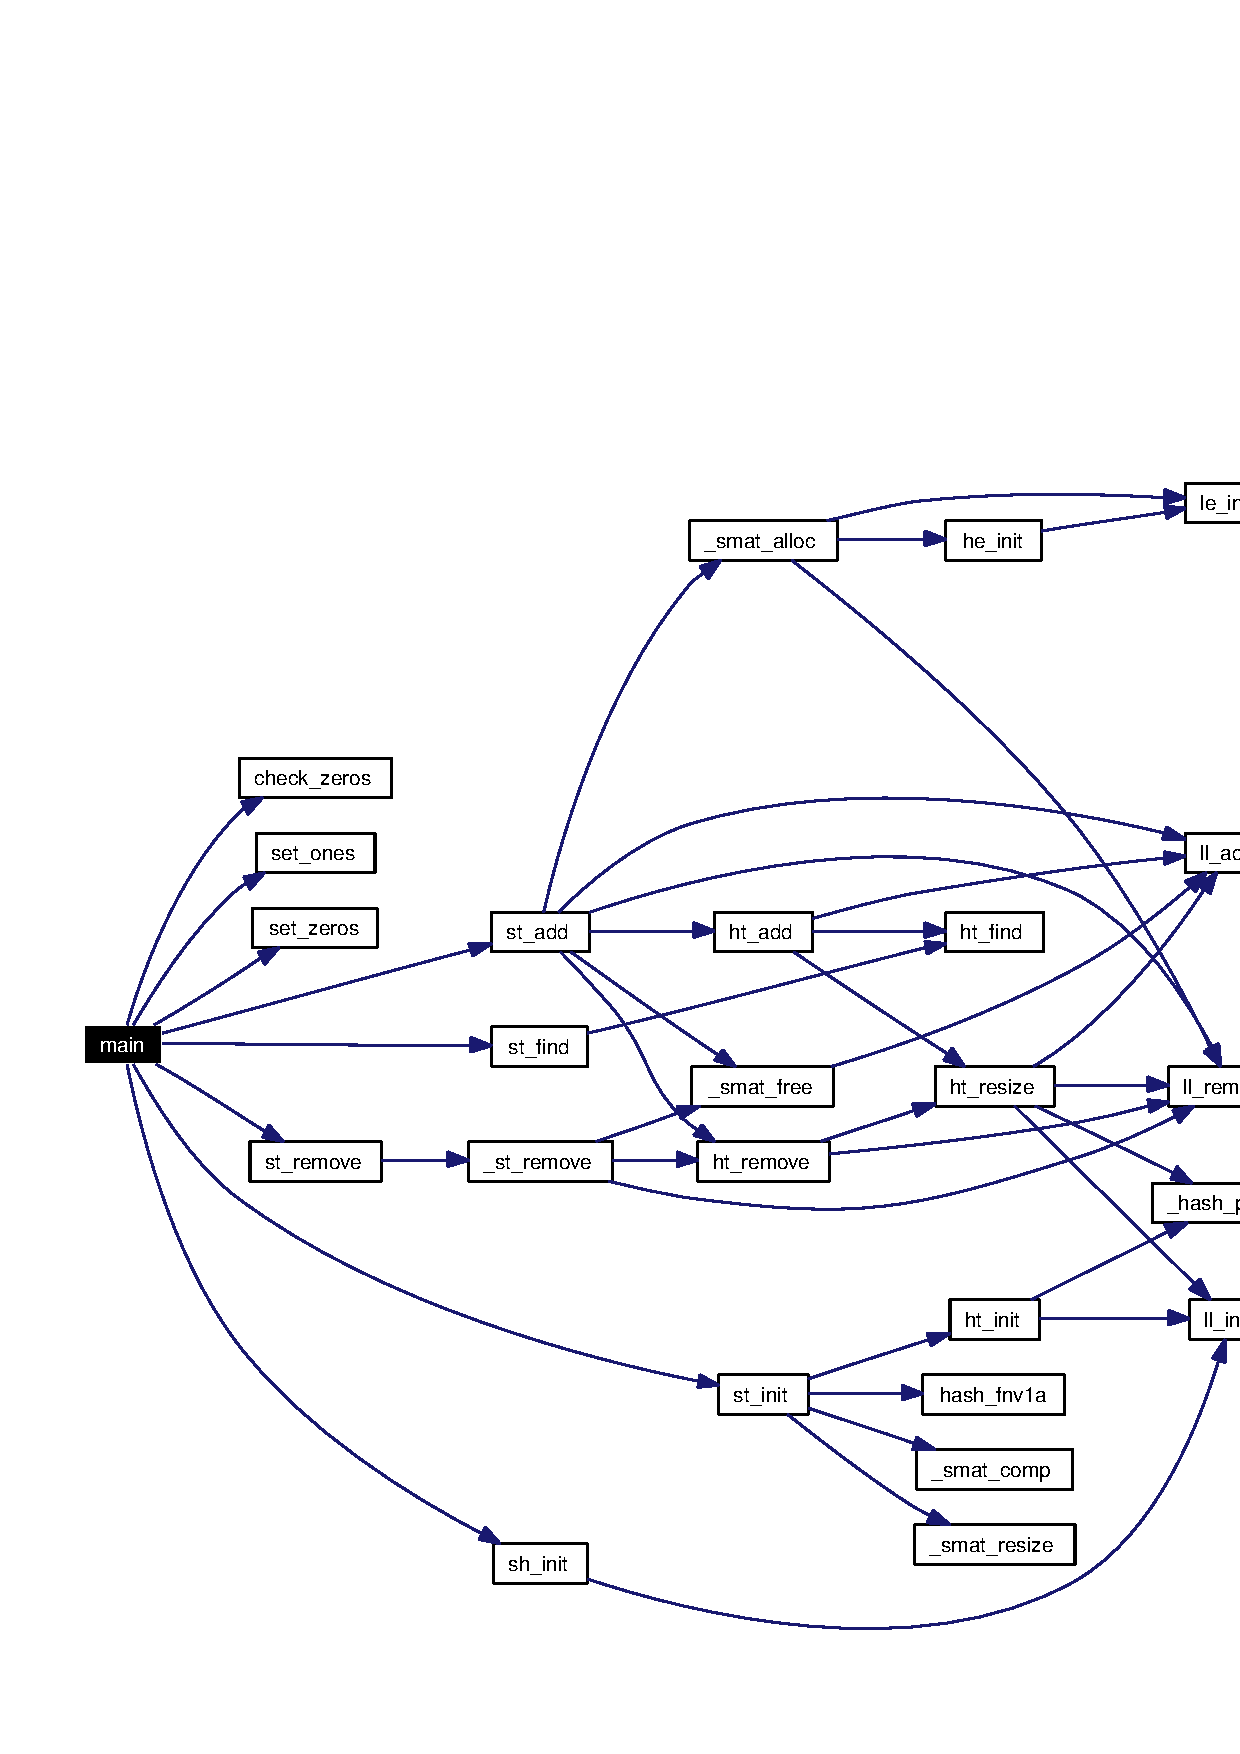
\includegraphics[width=316pt]{t__smat_8c_a12_cgraph}
\end{center}
\end{figure}
\hypertarget{t__smat_8c_a9}{
\index{t_smat.c@{t\_\-smat.c}!set_ones@{set\_\-ones}}
\index{set_ones@{set\_\-ones}!t_smat.c@{t\_\-smat.c}}
\subsubsection[set\_\-ones]{\setlength{\rightskip}{0pt plus 5cm}static void set\_\-ones (struct \hyperlink{structassoc__s}{assoc\_\-s} $\ast$ {\em assoc})\hspace{0.3cm}{\tt  \mbox{[}static\mbox{]}}}}
\label{t__smat_8c_a9}




Definition at line 52 of file t\_\-smat.c.

References assoc\_\-s::assoc, SMAT\_\-HEAD\_\-CNT, and SMAT\_\-HEAD\_\-MASK.

Referenced by main().\hypertarget{t__smat_8c_a10}{
\index{t_smat.c@{t\_\-smat.c}!set_zeros@{set\_\-zeros}}
\index{set_zeros@{set\_\-zeros}!t_smat.c@{t\_\-smat.c}}
\subsubsection[set\_\-zeros]{\setlength{\rightskip}{0pt plus 5cm}static void set\_\-zeros (struct \hyperlink{structassoc__s}{assoc\_\-s} $\ast$ {\em assoc})\hspace{0.3cm}{\tt  \mbox{[}static\mbox{]}}}}
\label{t__smat_8c_a10}




Definition at line 62 of file t\_\-smat.c.

References assoc\_\-s::assoc, and SMAT\_\-HEAD\_\-CNT.

Referenced by main().

\subsection{Variable Documentation}
\hypertarget{t__smat_8c_a8}{
\index{t_smat.c@{t\_\-smat.c}!associations@{associations}}
\index{associations@{associations}!t_smat.c@{t\_\-smat.c}}
\subsubsection[associations]{\setlength{\rightskip}{0pt plus 5cm}struct \hyperlink{structassoc__s}{assoc\_\-s}  \hyperlink{t__smat_8c_a8}{associations}\hspace{0.3cm}{\tt  \mbox{[}static\mbox{]}}}}
\label{t__smat_8c_a8}




Referenced by main().\hypertarget{t__smat_8c_a7}{
\index{t_smat.c@{t\_\-smat.c}!columns@{columns}}
\index{columns@{columns}!t_smat.c@{t\_\-smat.c}}
\subsubsection[columns]{\setlength{\rightskip}{0pt plus 5cm}\hyperlink{struct__smat__head__s}{smat\_\-head\_\-t} \hyperlink{t__smat_8c_a7}{columns}\mbox{[}SMAT\_\-HEAD\_\-CNT\mbox{]}\hspace{0.3cm}{\tt  \mbox{[}static\mbox{]}}}}
\label{t__smat_8c_a7}




Definition at line 43 of file t\_\-smat.c.\hypertarget{t__smat_8c_a6}{
\index{t_smat.c@{t\_\-smat.c}!rows@{rows}}
\index{rows@{rows}!t_smat.c@{t\_\-smat.c}}
\subsubsection[rows]{\setlength{\rightskip}{0pt plus 5cm}\hyperlink{struct__smat__head__s}{smat\_\-head\_\-t} \hyperlink{t__smat_8c_a6}{rows}\mbox{[}SMAT\_\-HEAD\_\-CNT\mbox{]}\hspace{0.3cm}{\tt  \mbox{[}static\mbox{]}}}}
\label{t__smat_8c_a6}




Definition at line 42 of file t\_\-smat.c.
\printindex
\end{document}
